\documentclass[11pt]{book}
\usepackage[T1]{fontenc}
\usepackage[utf8]{inputenc}
\usepackage{lmodern}
\usepackage{hyperref}
\usepackage{graphicx}
\usepackage[english]{babel}
\usepackage{listings}
\usepackage{amsmath}
\usepackage{amsthm}
\usepackage{amssymb}
\usepackage{natbib}
\usepackage{stmaryrd}
\usepackage{xypic}
\usepackage{semantic}
\usepackage{wrapfig}
\usepackage{multirow}
\usepackage{color}

\definecolor{lightgray}{gray}{1}
\newcommand{\black}[1]{{\color{black} #1}}
\newcommand{\gray}[1]{{\color{lightgray} #1}}

%% For pictures
\usepackage{tikz}
\usetikzlibrary{arrows.meta}
\tikzset{baseline=(current bounding box.center), >/.tip={Triangle[scale=1.4]}}

% Computer Modern is already the default. -Jeremy
%\renewcommand{\ttdefault}{cmtt}

\lstset{%
language=Lisp,
basicstyle=\ttfamily\small,
escapechar=|,
columns=flexible
}

\newtheorem{theorem}{Theorem}
\newtheorem{lemma}[theorem]{Lemma}
\newtheorem{corollary}[theorem]{Corollary}
\newtheorem{proposition}[theorem]{Proposition}
\newtheorem{constraint}[theorem]{Constraint}
\newtheorem{definition}[theorem]{Definition}
\newtheorem{exercise}[theorem]{Exercise}

%%%%%%%%%%%%%%%%%%%%%%%%%%%%%%%%%%%%%%%%%%%%%%%%%%%%%%%%%%%%%%%%%%%%%%%%%%%%%%%%
% 'dedication' environment: To add a dedication paragraph at the start of book %
% Source: http://www.tug.org/pipermail/texhax/2010-June/015184.html            %
%%%%%%%%%%%%%%%%%%%%%%%%%%%%%%%%%%%%%%%%%%%%%%%%%%%%%%%%%%%%%%%%%%%%%%%%%%%%%%%%
\newenvironment{dedication}
{
   \cleardoublepage
   \thispagestyle{empty}
   \vspace*{\stretch{1}}
   \hfill\begin{minipage}[t]{0.66\textwidth}
   \raggedright
}
{
   \end{minipage}
   \vspace*{\stretch{3}}
   \clearpage
}

%%%%%%%%%%%%%%%%%%%%%%%%%%%%%%%%%%%%%%%%%%%%%%%%
% Chapter quote at the start of chapter        %
% Source: http://tex.stackexchange.com/a/53380 %
%%%%%%%%%%%%%%%%%%%%%%%%%%%%%%%%%%%%%%%%%%%%%%%%
\makeatletter
\renewcommand{\@chapapp}{}% Not necessary...
\newenvironment{chapquote}[2][2em]
  {\setlength{\@tempdima}{#1}%
   \def\chapquote@author{#2}%
   \parshape 1 \@tempdima \dimexpr\textwidth-2\@tempdima\relax%
   \itshape}
  {\par\normalfont\hfill--\ \chapquote@author\hspace*{\@tempdima}\par\bigskip}
\makeatother

%%%%%%%%%%%%%%%%%%%%%%%%%%%%%%%%%%%%%%%%%%%%%%%%%%%%%%%%%%%%%%%%%%%%%%%%%%%%%%%%

\newcommand{\itm}[1]{\ensuremath{\mathit{#1}}}
\newcommand{\ttm}[1]{\ensuremath{\mathtt{#1}}}
\newcommand{\Stmt}{\itm{stmt}}
\newcommand{\Exp}{\itm{exp}}
\newcommand{\Def}{\itm{def}}
\newcommand{\Type}{\itm{type}}
\newcommand{\FType}{\itm{ftype}}
\newcommand{\Instr}{\itm{instr}}
\newcommand{\Block}{\itm{block}}
\newcommand{\Tail}{\itm{tail}}
\newcommand{\Prog}{\itm{prog}}
\newcommand{\Arg}{\itm{arg}}
\newcommand{\Atm}{\itm{atm}}
\newcommand{\Reg}{\itm{reg}}
\newcommand{\Int}{\itm{int}}
\newcommand{\Var}{\itm{var}}
\newcommand{\Op}{\itm{op}}
\newcommand{\key}[1]{\texttt{#1}}
\newcommand{\code}[1]{\texttt{#1}}

\newcommand{\LP}[0]{\key{(}}
\newcommand{\RP}[0]{\key{)}}
\newcommand{\LS}[0]{\key{[}}
\newcommand{\RS}[0]{\key{]}}
\newcommand{\INT}[1]{\key{(Int}\;#1\key{)}}
\newcommand{\BOOL}[1]{\key{(Bool}\;#1\key{)}}
\newcommand{\PRIM}[2]{\LP\key{Prim}~#1~\LP\key{list}~#2\RP\RP}
\newcommand{\READ}{\key{(Prim}\;\code{'read}\;\key{'())}}
\newcommand{\CREAD}{\key{(read)}}
\newcommand{\NEG}[1]{\key{(Prim}\;\code{'-}\;\code{(list}\;#1\;\code{))}}
\newcommand{\CNEG}[1]{\LP\key{-}~#1\RP}
\newcommand{\PROGRAM}[2]{\LP\code{Program}\;#1\;#2\RP}
\newcommand{\PROGRAMDEFSEXP}[3]{\code{(ProgramDefsExp}~#1~#2~#3\code{)}}
\newcommand{\PROGRAMDEFS}[2]{\code{(ProgramDefs}~#1~#2\code{)}}
\newcommand{\ADD}[2]{\key{(Prim}\;\code{'+}\;\code{(list}\;#1\;#2\code{))}}
\newcommand{\CADD}[2]{\LP\key{+}~#1~#2\RP}
\newcommand{\SUB}[2]{\key{(Prim}\;\code{'-}\;\code{(list}\;#1\;#2\code{))}}
\newcommand{\CSUB}[2]{\LP\key{-}~#1~#2\RP}
\newcommand{\CWHILE}[2]{\LP\key{while}~#1~#2\RP}
\newcommand{\WHILE}[2]{\LP\key{WhileLoop}~#1~#2\RP}
\newcommand{\CBEGIN}[2]{\LP\key{begin}~#1~#2\RP}
\newcommand{\BEGIN}[2]{\LP\key{Begin}~#1~#2\RP}
\newcommand{\CSETBANG}[2]{\LP\key{set!}~#1~#2\RP}
\newcommand{\SETBANG}[2]{\LP\key{SetBang}~#1~#2\RP}
\newcommand{\AND}[2]{\key{(Prim}\;\code{'and}\;\code{(list}\;#1\;#2\code{))}}
\newcommand{\OR}[2]{\key{(Prim}\;\code{'or}\;\code{(list}\;#1\;#2\code{))}}
\newcommand{\NOT}[1]{\key{(Prim}\;\code{'not}\;\code{(list}\;#1\;\code{))}}
\newcommand{\UNIOP}[2]{\key{(Prim}\;#1\;\code{(list}\;#2\code{))}}
\newcommand{\CUNIOP}[2]{\LP #1\;#2 \RP}
\newcommand{\BINOP}[3]{\key{(Prim}\;#1\;\code{(list}\;#2\;#3\code{))}}
\newcommand{\CBINOP}[3]{\LP #1\;#2\;#3\RP}
\newcommand{\CLET}[3]{\LP\key{let}~\LP\LS\Var~\Exp\RS\RP~\Exp\RP}
\newcommand{\CIF}[3]{\LP\key{if}~#1~#2~#3\RP}
\newcommand{\VAR}[1]{\key{(Var}\;#1\key{)}}
\newcommand{\LET}[3]{\key{(Let}~#1~#2~#3\key{)}}
\newcommand{\IF}[3]{\key{(If}\,#1\;#2\;#3\key{)}}
\newcommand{\VECTOR}[1]{\LP\key{Prim}\;\code{'vector}\;\LP\key{list}\;#1\RP\RP}
\newcommand{\VECREF}[2]{\LP\key{Prim}\;\code{'vector-ref}\;\LP\key{list}\;#1\;#2\RP\RP}
\newcommand{\VECSET}[3]{\LP\key{Prim}\;\code{'vector-set!}\;\LP\key{list}\;#1\;#2\;#3\RP\RP}
\newcommand{\VECLEN}[1]{\LP\key{Prim}\;\code{'vector-length}\;\LP\key{list}\;#1\RP\RP}
\newcommand{\CLOSURE}[2]{\LP\key{Closure}~#1~#2\RP}
\newcommand{\ALLOC}[2]{\LP\key{Allocate}~#1~#2\RP}
\newcommand{\ALLOCCLOS}[3]{\LP\key{AllocateClosure}~#1~#2~#3\RP}

\newcommand{\VOID}[1]{\key{(Void)}}
\newcommand{\APPLY}[2]{\key{(Apply}\;#1\;#2\code{)}}
\newcommand{\CALL}[2]{\key{(Call}\;#1\;#2\code{)}}
\newcommand{\TAILCALL}[2]{\key{(TailCall}\;#1\;#2\code{)}}
\newcommand{\FUNDEF}[5]{\key{(Def}~#1~#2~#3~#4~#5\code{)}}
\newcommand{\FUNREF}[1]{\key{(FunRef}\;#1\code{)}}
\newcommand{\CFUNREF}[1]{\key{(fun-ref}\;#1\code{)}}
\newcommand{\FUNREFARITY}[2]{\key{(FunRefArity}~#1~#2\code{)}}
\newcommand{\CFUNREFARITY}[2]{\key{(fun-ref-arity}~#1~#2\code{)}}
\newcommand{\LAMBDA}[3]{\key{(Lambda}~#1~#2~#3\code{)}}
\newcommand{\CLAMBDA}[3]{\LP\key{lambda:}\,#1\,\key{:}\,#2\;\Exp\RP}
\newcommand{\INJECT}[2]{\LP\key{Inject}~#1~#2\RP}
\newcommand{\PROJECT}[2]{\LP\key{Project}~#1~#2\RP}
\newcommand{\CINJECT}[2]{\LP\key{inject}~#1~#2\RP}
\newcommand{\CPROJECT}[2]{\LP\key{project}~#1~#2\RP}
\newcommand{\VALUEOF}[2]{\LP\key{ValueOf}~#1~#2\RP}

\newcommand{\ASSIGN}[2]{\key{(Assign}~#1\;#2\key{)}}
\newcommand{\RETURN}[1]{\key{(Return}~#1\key{)}}
\newcommand{\SEQ}[2]{\key{(Seq}~#1~#2\key{)}}
\newcommand{\GOTO}[1]{\key{(Goto}~#1\key{)}}
\newcommand{\IFSTMT}[3]{\key{(IfStmt}\,#1\;#2\;#3\key{)}}

\newcommand{\IMM}[1]{\key{(Imm}\;#1\key{)}}
\newcommand{\REG}[1]{\key{(Reg}\;#1\key{)}}
\newcommand{\BYTEREG}[1]{\key{(ByteReg}\;#1\key{)}}
\newcommand{\DEREF}[2]{\key{(Deref}~#1~#2\key{)}}
\newcommand{\DEF}[5]{\key{(Def}~#1~#2~#3~#4~#5\key{)}}
\newcommand{\CDEF}[4]{\LP\key{define}~\LP#1~#2\RP\,\key{:}\,#3~#4\RP}
\newcommand{\CFG}[1]{\key{(CFG}\;#1\key{)}}
\newcommand{\BLOCK}[2]{\key{(Block}\;#1\;#2\key{)}}
\newcommand{\STACKLOC}[1]{(\key{stack}\;#1)}
\newcommand{\BININSTR}[3]{\key{(Instr}\;#1\;\key{(list}\;#2\;#3\key{))}}
\newcommand{\UNIINSTR}[2]{\key{(Instr}\;#1\;\key{(list}\;#2\key{))}}
\newcommand{\CALLQ}[2]{\key{(Callq}~#1~#2\key{)}}
\newcommand{\INDCALLQ}[2]{\key{(IndirectCallq}~#1~#2\key{)}}
\newcommand{\RETQ}{\key{(Retq)}}
\newcommand{\PUSHQ}[1]{\key{(Pushq}~#1\key{)}}
\newcommand{\POPQ}[1]{\key{(Popq}~#1\key{)}}
\newcommand{\JMP}[1]{\key{(Jmp}~#1\key{)}}
\newcommand{\TAILJMP}[2]{\key{(TailJmp}~#1~#2\key{)}}
\newcommand{\JMPIF}[2]{\key{(JmpIf}~#1~#2\key{)}}



\newcommand{\TTKEY}[1]{{\normalfont\tt #1}}



%%%%%%%%%%%%%%%%%%%%%%%%%%%%%%%%%%%%%%%%%%%%%%%%%%%%%%%%%%%%%%%%%%%%%%%%%%%%%%%%

\title{\Huge \textbf{Essentials of Compilation} \\ 
  \huge An Incremental Approach}

\author{\textsc{Jeremy G. Siek} \\
%\thanks{\url{http://homes.soic.indiana.edu/jsiek/}} \\
  Indiana University \\
  \\
  with contributions from: \\
  Carl Factora \\
  Michael M. Vitousek \\
  Cameron Swords
   }

\begin{document}

\frontmatter
\maketitle

\begin{dedication}
This book is dedicated to the programming language wonks at Indiana
University.
\end{dedication}

\tableofcontents
%\listoffigures
%\listoftables

\mainmatter

%%%%%%%%%%%%%%%%%%%%%%%%%%%%%%%%%%%%%%%%%%%%%%%%%%%%%%%%%%%%%%%%%%%%%%%%%%%%%%%%
\chapter*{Preface}

The tradition of compiler writing at Indiana University goes back to
programming language research and courses taught by Daniel Friedman in
the 1970's and 1980's. Dan had conducted research on lazy evaluation
in the context of Lisp~\citep{McCarthy:1960dz} and then studied
continuations and macros in the context of the
Scheme~\citep{Sussman:1975ab}, a dialect of Lisp.  One of students of
those courses, Kent Dybvig, went on to build Chez
Scheme~\citep{Dybvig:2006aa}, a production-quality and efficient
compiler for Scheme. After completing his Ph.D. at the University of
North Carolina, Kent returned to teach at Indiana University.
Throughout the 1990's and early 2000's, Kent continued development of
Chez Scheme and rotated with Dan in teaching the compiler course.

Thanks to this collaboration between Dan and Kent, the compiler course
evolved to incorporate novel pedagogical ideas while also including
elements of effective real-world compilers.  One of Dan's ideas was to
split the compiler into many small passes over the input program and
subsequent intermediate representations, so that the code for each
pass would be easy to understood in isolation.  (In contrast, most
compilers of the time were organized into only a few monolithic passes
for reasons of compile-time efficiency.)  Kent and his students,
Dipanwita Sarkar and Andrew Keep, developed infrastructure to support
this approach and evolved the course, first to use micro-sized passes
and then into even smaller nano
passes~\citep{Sarkar:2004fk,Keep:2012aa}. I took this compiler course
in the early 2000's, as part of my Ph.D. studies at Indiana
University. Needless to say, I enjoyed the course immensely.

One of my classmates, Abdulaziz Ghuloum, observed that the
front-to-back organization of the course made it difficult for
students to understand the rationale for the compiler
design. Abdulaziz proposed an incremental approach in which the
students build the compiler in stages; they start by implementing a
complete compiler for a very small subset of the input language, then
in each subsequent stage they add a feature to the input language and
add or modify passes to handle the new feature~\citep{Ghuloum:2006bh}.
In this way, the students see how the language features motivate
aspects of the compiler design.

After graduating from Indiana University in 2005, I went on to teach
at the University of Colorado. I adapted the nano pass and incremental
approaches to compiling a subset of the Python
language~\citep{Siek:2012ab}.  Python and Scheme are quite different
on the surface but there is a large overlap in the compiler techniques
required for the two languages. Thus, I was able to teach much of the
same content from the Indiana compiler course. I very much enjoyed
teaching the course organized in this way, and even better, many of
the students learned a lot and got excited about compilers.  (No, I
didn't do a quantitative study to support this claim.)

It is now 2016 and I too have returned to teach at Indiana University.
In my absence the compiler course had switched from the front-to-back
organization to a back-to-front organization. Seeing how well the
incremental approach worked at Colorado, I found this unsatisfactory
and have reorganized the course, porting and adapting the structure of
the Colorado course back into the land of Scheme. In the meantime
Scheme has been superseded by Racket (at least in Indiana), so the
course is now about compiling a subset of Racket to the x86 assembly
language and the compiler is implemented in Racket~\citep{plt-tr}.

This is the textbook for the incremental version of the compiler
course at Indiana University (Spring 2016) and it is the first
textbook for an Indiana compiler course.  With this book I hope to
make the Indiana compiler course available to people that have not had
the chance to study here in person.  Many of the compiler design
decisions in this book are drawn from the assignment descriptions of
\cite{Dybvig:2010aa}. I have captured what I think are the most
important topics from \cite{Dybvig:2010aa} but have omitted topics
that I think are less interesting conceptually and I have made
simplifications to reduce complexity.  In this way, this book leans
more towards pedagogy than towards absolute efficiency. Also, the book
differs in places where I saw the opportunity to make the topics more
fun, such as in relating register allocation to Sudoku
(Chapter~\ref{ch:register-allocation}).

\section*{Prerequisites}

The material in this book is challenging but rewarding. It is meant to
prepare students for a lifelong career in programming languages.  I do
not recommend this book for students who want to dabble in programming
languages.  Because the book uses the Racket language both for the
implementation of the compiler and for the language that is compiled,
a student should be proficient with Racket (or Scheme) prior to
reading this book. There are many other excellent resources for
learning Scheme and
Racket~\citep{Dybvig:1987aa,Abelson:1996uq,Friedman:1996aa,Felleisen:2001aa,Felleisen:2013aa,Flatt:2014aa}. It
is helpful but not necessary for the student to have prior exposure to
x86 (or x86-64) assembly language~\citep{Intel:2015aa}, as one might
obtain from a computer systems
course~\citep{Bryant:2005aa,Bryant:2010aa}.  This book introduces the
parts of x86-64 assembly language that are needed.

%\section*{Structure of book}
% You might want to add short description about each chapter in this book.

%\section*{About the companion website}
%The website\footnote{\url{https://github.com/amberj/latex-book-template}} for %this file contains:
%\begin{itemize}
%  \item A link to (freely downlodable) latest version of this document.
%  \item Link to download LaTeX source for this document.
%  \item Miscellaneous material (e.g. suggested readings etc).
%\end{itemize}

\section*{Acknowledgments}

Need to give thanks to 
\begin{itemize}
\item Bor-Yuh Evan Chang
\item Kent Dybvig
\item Daniel P. Friedman
\item Ronald Garcia
\item Abdulaziz Ghuloum
\item Ryan Newton
\item Dipanwita Sarkar
\item Andrew Keep
\item Oscar Waddell
\end{itemize}

\mbox{}\\
\noindent Jeremy G. Siek \\
\noindent \url{http://homes.soic.indiana.edu/jsiek} \\
\noindent Spring 2016 

%%%%%%%%%%%%%%%%%%%%%%%%%%%%%%%%%%%%%%%%%%%%%%%%%%%%%%%%%%%%%%%%%%%%%%%%%%%%%%%%
\chapter{Preliminaries}
\label{ch:trees-recur}

In this chapter, we review the basic tools that are needed for
implementing a compiler. We use abstract syntax trees (ASTs) in the
form of S-expressions to represent programs (Section~\ref{sec:ast})
and pattern matching to inspect individual nodes in an AST
(Section~\ref{sec:pattern-matching}).  We use recursion to construct
and deconstruct entire ASTs (Section~\ref{sec:recursion}).

\section{Abstract Syntax Trees}
\label{sec:ast}

The primary data structure that is commonly used for representing
programs is the \emph{abstract syntax tree} (AST). When considering
some part of a program, a compiler needs to ask what kind of part it
is and what sub-parts it has. For example, the program on the left is
represented by the AST on the right.
\begin{center}
\begin{minipage}{0.4\textwidth}
\begin{lstlisting}
(+ (read) (- 8))
\end{lstlisting}
\end{minipage}
\begin{minipage}{0.4\textwidth}
\begin{equation}
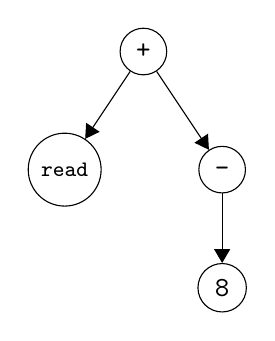
\begin{tikzpicture}
 \node[draw, circle] (plus)  at (0 ,  0) {\key{+}};
 \node[draw, circle] (read)  at (-1, -1.5) {{\footnotesize\key{read}}};
 \node[draw, circle] (minus) at (1 , -1.5) {$\key{-}$};
 \node[draw, circle] (8)     at (1 , -3) {\key{8}};

 \draw[->] (plus) to (read);
 \draw[->] (plus) to (minus);
 \draw[->] (minus) to (8);
\end{tikzpicture}
\label{eq:arith-prog}
\end{equation}
\end{minipage}
\end{center}
We shall use the standard terminology for trees: each circle above is
called a \emph{node}. The arrows connect a node to its \emph{children}
(which are also nodes). The top-most node is the \emph{root}.  Every
node except for the root has a \emph{parent} (the node it is the child
of). If a node has no children, it is a \emph{leaf} node.  Otherwise
it is an \emph{internal} node.

When deciding how to compile the above program, we need to know that
the root node operation is addition and that it has two children:
\texttt{read} and a negation. The abstract syntax tree data structure
directly supports these queries and hence is a good choice. In this
book, we will often write down the textual representation of a program
even when we really have in mind the AST because the textual
representation is more concise.  We recommend that, in your mind, you
always interpret programs as abstract syntax trees.

\section{Grammars}
\label{sec:grammar}

A programming language can be thought of as a \emph{set} of programs.
The set is typically infinite (one can always create larger and larger
programs), so one cannot simply describe a language by listing all of
the programs in the language. Instead we write down a set of rules, a
\emph{grammar}, for building programs. We shall write our rules in a
variant of Backus-Naur Form (BNF)~\citep{Backus:1960aa,Knuth:1964aa}.
As an example, we describe a small language, named $R_0$, of
integers and arithmetic operations. The first rule says that any
integer is an expression, $\Exp$, in the language:
\begin{equation}
\Exp ::= \Int  \label{eq:arith-int}
\end{equation}
Each rule has a left-hand-side and a right-hand-side. The way to read
a rule is that if you have all the program parts on the
right-hand-side, then you can create an AST node and categorize it
according to the left-hand-side. (We do not define $\Int$ because the
reader already knows what an integer is.) We make the simplifying
design decision that all of the languages in this book only handle
machine-representable integers (those representable with 64-bits,
i.e., the range $-2^{63}$ to $2^{63}$) which corresponds to the
\texttt{fixnum} datatype in Racket. A name such as $\Exp$ that is
defined by the grammar rules is a \emph{non-terminal}.

The second grammar rule is the \texttt{read} operation that receives
an input integer from the user of the program.
\begin{equation}
  \Exp ::= (\key{read}) \label{eq:arith-read}
\end{equation}

The third rule says that, given an $\Exp$ node, you can build another
$\Exp$ node by negating it.
\begin{equation}
  \Exp ::= (\key{-} \; \Exp)  \label{eq:arith-neg}
\end{equation}
Symbols such as \key{-} in typewriter font are \emph{terminal} symbols
and must literally appear in the program for the rule to be
applicable.

We can apply the rules to build ASTs in the $R_0$
language. For example, by rule \eqref{eq:arith-int}, \texttt{8} is an
$\Exp$, then by rule \eqref{eq:arith-neg}, the following AST is
an $\Exp$.
\begin{center}
\begin{minipage}{0.25\textwidth}
\begin{lstlisting}
(- 8)
\end{lstlisting}
\end{minipage}
\begin{minipage}{0.25\textwidth}
\begin{equation}
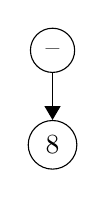
\begin{tikzpicture}
 \node[draw, circle] (minus) at (0, 0)  {$\text{--}$};
 \node[draw, circle] (8)     at (0, -1.2) {$8$};

 \draw[->] (minus) to (8);
\end{tikzpicture}
\label{eq:arith-neg8}
\end{equation}
\end{minipage}
\end{center}

The following grammar rule defines addition expressions:
\begin{equation}
  \Exp ::= (\key{+} \; \Exp \; \Exp) \label{eq:arith-add}
\end{equation}
Now we can see that the AST \eqref{eq:arith-prog} is an $\Exp$ in
$R_0$.  We know that \lstinline{(read)} is an $\Exp$ by rule
\eqref{eq:arith-read} and we have shown that \texttt{(- 8)} is an
$\Exp$, so we can apply rule \eqref{eq:arith-add} to show that
\texttt{(+ (read) (- 8))} is an $\Exp$ in the $R_0$ language.

If you have an AST for which the above rules do not apply, then the
AST is not in $R_0$. For example, the AST \texttt{(- (read) (+ 8))} is
not in $R_0$ because there are no rules for \key{+} with only one
argument, nor for \key{-} with two arguments.  Whenever we define a
language with a grammar, we implicitly mean for the language to be the
smallest set of programs that are justified by the rules. That is, the
language only includes those programs that the rules allow.

The last grammar for $R_0$ states that there is a \key{program} node
to mark the top of the whole program:
\[
  R_0 ::= (\key{program} \; \Exp)
\]

The \code{read-program} function provided in \code{utilities.rkt}
reads programs in from a file (the sequence of characters in the
concrete syntax of Racket) and parses them into the abstract syntax
tree. The concrete syntax does not include a \key{program} form; that
is added by the \code{read-program} function as it creates the
AST. See the description of \code{read-program} in
Appendix~\ref{appendix:utilities} for more details.

It is common to have many rules with the same left-hand side, such as
$\Exp$ in the grammar for $R_0$, so there is a vertical bar notation
for gathering several rules, as shown in
Figure~\ref{fig:r0-syntax}. Each clause between a vertical bar is
called an {\em alternative}.

\begin{figure}[tbp]
\fbox{
\begin{minipage}{0.96\textwidth}
\[
\begin{array}{rcl}
\Exp &::=& \Int \mid ({\tt \key{read}}) \mid (\key{-} \; \Exp) \mid
   (\key{+} \; \Exp \; \Exp)  \\
R_0  &::=& (\key{program} \; \Exp)
\end{array}
\]
\end{minipage}
}
\caption{The syntax of the $R_0$ language.}
\label{fig:r0-syntax}
\end{figure}

\section{S-Expressions}
\label{sec:s-expr}

Racket, as a descendant of Lisp, has
convenient support for creating and manipulating abstract syntax trees
with its \emph{symbolic expression} feature, or S-expression for
short. We can create an S-expression simply by writing a backquote
followed by the textual representation of the AST. (Technically
speaking, this is called a \emph{quasiquote} in Racket.)  For example,
an S-expression to represent the AST \eqref{eq:arith-prog} is created
by the following Racket expression:
\begin{center}
\texttt{`(+ (read) (- 8))}
\end{center}

To build larger S-expressions one often needs to splice together
several smaller S-expressions. Racket provides the comma operator to
splice an S-expression into a larger one. For example, instead of
creating the S-expression for AST \eqref{eq:arith-prog} all at once,
we could have first created an S-expression for AST
\eqref{eq:arith-neg8} and then spliced that into the addition
S-expression.
\begin{lstlisting}
   (define ast1.4 `(- 8))
   (define ast1.1 `(+ (read) ,ast1.4))
\end{lstlisting}
In general, the Racket expression that follows the comma (splice)
can be any expression that computes an S-expression.

\section{Pattern Matching}
\label{sec:pattern-matching}

As mentioned above, one of the operations that a compiler needs to
perform on an AST is to access the children of a node.  Racket
provides the \texttt{match} form to access the parts of an
S-expression. Consider the following example and the output on the
right.
\begin{center}
\begin{minipage}{0.5\textwidth}
\begin{lstlisting}
(match ast1.1
  [`(,op ,child1 ,child2)
    (print op) (newline)
    (print child1) (newline)
    (print child2)])
\end{lstlisting}
\end{minipage}
\vrule
\begin{minipage}{0.25\textwidth}
\begin{lstlisting}


   '+
   '(read)
   '(- 8)
\end{lstlisting}
\end{minipage}
\end{center}
The \texttt{match} form takes AST \eqref{eq:arith-prog} and binds its
parts to the three variables \texttt{op}, \texttt{child1}, and
\texttt{child2}. In general, a match clause consists of a
\emph{pattern} and a \emph{body}. The pattern is a quoted S-expression
that may contain pattern-variables (preceded by a comma).  The body
may contain any Racket code.

A \texttt{match} form may contain several clauses, as in the following
function \texttt{leaf?} that recognizes when an $R_0$ node is
a leaf. The \texttt{match} proceeds through the clauses in order,
checking whether the pattern can match the input S-expression. The
body of the first clause that matches is executed. The output of
\texttt{leaf?} for several S-expressions is shown on the right. In the
below \texttt{match}, we see another form of pattern: the \texttt{(?
  fixnum?)} applies the predicate \texttt{fixnum?} to the input
S-expression to see if it is a machine-representable integer.
\begin{center}
\begin{minipage}{0.5\textwidth}
\begin{lstlisting}
(define (leaf? arith)
  (match arith
    [(? fixnum?) #t]
    [`(read) #t]
    [`(- ,c1) #f]
    [`(+ ,c1 ,c2) #f]))

(leaf? `(read))
(leaf? `(- 8))
(leaf? `(+ (read) (- 8)))
\end{lstlisting}
\end{minipage}
\vrule
\begin{minipage}{0.25\textwidth}
\begin{lstlisting}






   #t
   #f
   #f
\end{lstlisting}
\end{minipage}
\end{center}


\section{Recursion}
\label{sec:recursion}

Programs are inherently recursive in that an $R_0$ AST is made
up of smaller $R_0$ ASTs. Thus, the natural way to process in
entire program is with a recursive function.  As a first example of
such a function, we define \texttt{R0?} below, which takes an
arbitrary S-expression, {\tt sexp}, and determines whether or not {\tt
  sexp} is in {\tt arith}. Note that each match clause corresponds to
one grammar rule for $R_0$ and the body of each clause makes a
recursive call for each child node. This pattern of recursive function
is so common that it has a name, \emph{structural recursion}.  In
general, when a recursive function is defined using a sequence of
match clauses that correspond to a grammar, and each clause body makes
a recursive call on each child node, then we say the function is
defined by structural recursion.
\begin{center}
\begin{minipage}{0.7\textwidth}
\begin{lstlisting}
(define (R0? sexp)
  (match sexp
    [(? fixnum?) #t]
    [`(read) #t]
    [`(- ,e) (R0? e)]
    [`(+ ,e1 ,e2)
     (and (R0? e1) (R0? e2))]
    [`(program ,e) (R0? e)]
    [else #f]))

(R0? `(+ (read) (- 8)))
(R0? `(- (read) (+ 8)))
\end{lstlisting}
\end{minipage}
\vrule
\begin{minipage}{0.25\textwidth}
\begin{lstlisting}








   #t
   #f
\end{lstlisting}
\end{minipage}
\end{center}



\section{Interpreters}
\label{sec:interp-R0}

The meaning, or semantics, of a program is typically defined in the
specification of the language. For example, the Scheme language is
defined in the report by \cite{SPERBER:2009aa}. The Racket language is
defined in its reference manual~\citep{plt-tr}. In this book we use an
interpreter to define the meaning of each language that we consider,
following Reynold's advice in this
regard~\citep{reynolds72:_def_interp}. Here we will warm up by writing
an interpreter for the $R_0$ language, which will also serve
as a second example of structural recursion. The \texttt{interp-R0}
function is defined in Figure~\ref{fig:interp-R0}. The body of the
function is a match on the input expression \texttt{e} and there is
one clause per grammar rule for $R_0$. The clauses for
internal AST nodes make recursive calls to \texttt{interp-R0} on
each child node.

\begin{figure}[tbp]
\begin{lstlisting}
   (define (interp-R0 e)
     (match e
       [(? fixnum?) e]
       [`(read)
        (define r (read))
        (cond [(fixnum? r) r]
              [else (error 'interp-R0 "expected an integer" r)])]
       [`(- ,e)
        (fx- 0 (interp-R0 e))]
       [`(+ ,e1 ,e2)
        (fx+ (interp-R0 e1) (interp-R0 e2))]
       [`(program ,e) (interp-R0 e)]
       ))
\end{lstlisting}
\caption{Interpreter for the $R_0$ language.}
\label{fig:interp-R0}
\end{figure}

Let us consider the result of interpreting some example $R_0$
programs. The following program simply adds two integers.
\begin{lstlisting}
   (+ 10 32)
\end{lstlisting}
The result is \key{42}, as you might have expected. 
%
The next example demonstrates that expressions may be nested within
each other, in this case nesting several additions and negations.
\begin{lstlisting}
   (+ 10 (- (+ 12 20)))
\end{lstlisting}
What is the result of the above program?

If we interpret the AST \eqref{eq:arith-prog} and give it the input
\texttt{50}
\begin{lstlisting}
   (interp-R0 ast1.1)
\end{lstlisting}
we get the answer to life, the universe, and everything:
\begin{lstlisting}
   42
\end{lstlisting}

Moving on, the \key{read} operation prompts the user of the program
for an integer. Given an input of \key{10}, the following program
produces \key{42}.
\begin{lstlisting}
   (+ (read) 32)
\end{lstlisting}
We include the \key{read} operation in $R_1$ so that a compiler for
$R_1$ cannot be implemented simply by running the interpreter at
compilation time to obtain the output and then generating the trivial
code to return the output. (A clever student at Colorado did this the
first time I taught the course.)

The job of a compiler is to translate a program in one language into a
program in another language so that the output program behaves the
same way as the input program. This idea is depicted in the following
diagram. Suppose we have two languages, $\mathcal{L}_1$ and
$\mathcal{L}_2$, and an interpreter for each language.  Suppose that
the compiler translates program $P_1$ in language $\mathcal{L}_1$ into
program $P_2$ in language $\mathcal{L}_2$.  Then interpreting $P_1$
and $P_2$ on their respective interpreters with input $i$ should yield
the same output $o$.
\begin{equation} \label{eq:compile-correct}
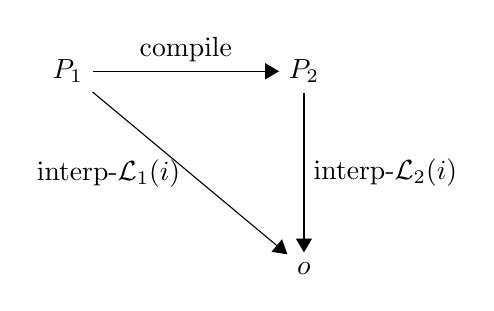
\begin{tikzpicture}[baseline=(current  bounding  box.center)]
 \node (p1) at (0,  0) {$P_1$};
 \node (p2) at (3,  0) {$P_2$};
 \node (o)  at (3, -2.5) {$o$};

 \path[->] (p1) edge [above] node {compile} (p2);
 \path[->] (p2) edge [right] node {interp-$\mathcal{L}_2$($i$)} (o);
 \path[->] (p1) edge [left]  node {interp-$\mathcal{L}_1$($i$)} (o);
\end{tikzpicture}
\end{equation}
In the next section we see our first example of a compiler, which is
another example of structural recursion.


\section{Partial Evaluation}
\label{sec:partial-evaluation}

In this section we consider a compiler that translates $R_0$
programs into $R_0$ programs that are more efficient, that is,
this compiler is an optimizer. Our optimizer will accomplish this by
trying to eagerly compute the parts of the program that do not depend
on any inputs. For example, given the following program
\begin{lstlisting}
   (+ (read) (- (+ 5 3)))
\end{lstlisting}
our compiler will translate it into the program
\begin{lstlisting}
   (+ (read) -8)
\end{lstlisting}

Figure~\ref{fig:pe-arith} gives the code for a simple partial
evaluator for the $R_0$ language. The output of the partial evaluator
is an $R_0$ program, which we build up using a combination of
quasiquotes and commas. (Though no quasiquote is necessary for
integers.) In Figure~\ref{fig:pe-arith}, the normal structural
recursion is captured in the main \texttt{pe-arith} function whereas
the code for partially evaluating negation and addition is factored
into two separate helper functions: \texttt{pe-neg} and
\texttt{pe-add}. The input to these helper functions is the output of
partially evaluating the children nodes.

\begin{figure}[tbp]
\begin{lstlisting}
   (define (pe-neg r)
     (cond [(fixnum? r) (fx- 0 r)]
           [else `(- ,r)]))
   (define (pe-add r1 r2)
     (cond [(and (fixnum? r1) (fixnum? r2)) (fx+ r1 r2)]
           [else `(+ ,r1 ,r2)]))
   (define (pe-arith e)
     (match e
       [(? fixnum?) e]
       [`(read) `(read)]
       [`(- ,e1) (pe-neg (pe-arith e1))]
       [`(+ ,e1 ,e2) (pe-add (pe-arith e1) (pe-arith e2))]))   
\end{lstlisting}
\caption{A partial evaluator for the $R_0$ language.}
\label{fig:pe-arith}
\end{figure}

Our code for \texttt{pe-neg} and \texttt{pe-add} implements the simple
idea of checking whether the inputs are integers and if they are, to
go ahead and perform the arithmetic.  Otherwise, we use quasiquote to
create an AST node for the appropriate operation (either negation or
addition) and use comma to splice in the child nodes.

To gain some confidence that the partial evaluator is correct, we can
test whether it produces programs that get the same result as the
input program. That is, we can test whether it satisfies Diagram
\eqref{eq:compile-correct}. The following code runs the partial
evaluator on several examples and tests the output program.  The
\texttt{assert} function is defined in Appendix~\ref{appendix:utilities}.
\begin{lstlisting}
(define (test-pe p)
  (assert "testing pe-arith"
     (equal? (interp-R0 p) (interp-R0 (pe-arith p)))))

(test-pe `(+ (read) (- (+ 5 3))))
(test-pe `(+ 1 (+ (read) 1)))
(test-pe `(- (+ (read) (- 5))))
\end{lstlisting}

\begin{exercise}
\normalfont % I don't like the italics for exercises. -Jeremy
We challenge the reader to improve on the simple partial evaluator in
Figure~\ref{fig:pe-arith} by replacing the \texttt{pe-neg} and
\texttt{pe-add} helper functions with functions that know more about
arithmetic. For example, your partial evaluator should translate
\begin{lstlisting}
   (+ 1 (+ (read) 1))
\end{lstlisting}
into
\begin{lstlisting}
   (+ 2 (read))
\end{lstlisting}
To accomplish this, we recommend that your partial evaluator produce
output that takes the form of the $\itm{residual}$ non-terminal in the
following grammar.
\[
\begin{array}{lcl}
\Exp &::=& (\key{read}) \mid (\key{-} \;(\key{read})) \mid (\key{+} \; \Exp \; \Exp)\\
\itm{residual} &::=& \Int \mid (\key{+}\; \Int\; \Exp) \mid \Exp
\end{array}
\]
\end{exercise}


%%%%%%%%%%%%%%%%%%%%%%%%%%%%%%%%%%%%%%%%%%%%%%%%%%%%%%%%%%%%%%%%%%%%%%%%%%%%%%%%
\chapter{Compiling Integers and Variables}
\label{ch:int-exp}

This chapter concerns the challenge of compiling a subset of Racket,
which we name $R_1$, to x86-64 assembly code~\citep{Intel:2015aa}.
(Henceforce we shall refer to x86-64 simply as x86).  The chapter
begins with a description of the $R_1$ language (Section~\ref{sec:s0})
and then a description of x86 (Section~\ref{sec:x86}). The
x86 assembly language is quite large, so we only discuss what is
needed for compiling $R_1$. We introduce more of x86 in later
chapters. Once we have introduced $R_1$ and x86, we reflect on
their differences and come up with a plan breaking down the
translation from $R_1$ to x86 into a handful of steps
(Section~\ref{sec:plan-s0-x86}).  The rest of the sections in this
Chapter give detailed hints regarding each step
(Sections~\ref{sec:uniquify-s0} through \ref{sec:patch-s0}).  We hope
to give enough hints that the well-prepared reader can implement a
compiler from $R_1$ to x86 while at the same time leaving room for
some fun and creativity.

\section{The $R_1$ Language}
\label{sec:s0}

The $R_1$ language extends the $R_0$ language
(Figure~\ref{fig:r0-syntax}) with variable definitions.  The syntax of
the $R_1$ language is defined by the grammar in
Figure~\ref{fig:r1-syntax}. As in $R_0$, \key{read} is a nullary
operator, \key{-} is a unary operator, and \key{+} is a binary
operator. In addition to variable definitions, the $R_1$ language
includes the \key{program} form to mark the top of the program, which
is helpful in some of the compiler passes.  The $R_1$ language is rich
enough to exhibit several compilation techniques but simple enough so
that the reader can implement a compiler for it in a week of part-time
work.  To give the reader a feeling for the scale of this first
compiler, the instructor solution for the $R_1$ compiler consists of 6
recursive functions and a few small helper functions that together
span 256 lines of code.

\begin{figure}[btp]
\centering
\fbox{
\begin{minipage}{0.96\textwidth}
\[
\begin{array}{rcl}
\Exp &::=& \Int \mid (\key{read}) \mid (\key{-}\;\Exp) \mid (\key{+} \; \Exp\;\Exp)  \\
     &\mid&  \Var \mid \LET{\Var}{\Exp}{\Exp} \\
R_1  &::=& (\key{program} \; \Exp)
\end{array}
\]
\end{minipage}
}
\caption{The syntax of the $R_1$ language. 
  The non-terminal \Var{} may be any Racket identifier.}
\label{fig:r1-syntax}
\end{figure}

The \key{let} construct defines a variable for use within its body
and initializes the variable with the value of an expression.  So the
following program initializes \code{x} to \code{32} and then evaluates
the body \code{(+ 10 x)}, producing \code{42}.
\begin{lstlisting}
   (program
      (let ([x (+ 12 20)]) (+ 10 x)))
\end{lstlisting}
When there are multiple \key{let}'s for the same variable, the closest
enclosing \key{let} is used. That is, variable definitions overshadow
prior definitions. Consider the following program with two \key{let}'s
that define variables named \code{x}. Can you figure out the result?
\begin{lstlisting}
   (program
      (let ([x 32]) (+ (let ([x 10]) x) x)))
\end{lstlisting}
For the purposes of showing which variable uses correspond to which
definitions, the following shows the \code{x}'s annotated with subscripts
to distinguish them. Double check that your answer for the above is
the same as your answer for this annotated version of the program.
\begin{lstlisting}
   (program
      (let ([x|$_1$| 32]) (+ (let ([x|$_2$| 10]) x|$_2$|) x|$_1$|)))
\end{lstlisting}
The initializing expression is always evaluated before the body of the
\key{let}, so in the following, the \key{read} for \code{x} is
performed before the \key{read} for \code{y}. Given the input
\code{52} then \code{10}, the following produces \code{42} (and not
\code{-42}).
\begin{lstlisting}
   (program
     (let ([x (read)]) (let ([y (read)]) (- x y))))
\end{lstlisting}

Figure~\ref{fig:interp-R1} shows the interpreter for the $R_1$
language. It extends the interpreter for $R_0$ with two new
\key{match} clauses for variables and for \key{let}.  For \key{let},
we will need a way to communicate the initializing value of a variable
to all the uses of a variable. To accomplish this, we maintain a
mapping from variables to values, which is traditionally called an
\emph{environment}. For simplicity, here we use an association list to
represent the environment. The \code{interp-R1} function takes the
current environment, \code{env}, as an extra parameter.  When the
interpreter encounters a variable, it finds the corresponding value
using the \code{lookup} function (Appendix~\ref{appendix:utilities}).
When the interpreter encounters a \key{let}, it evaluates the
initializing expression, extends the environment with the result bound
to the variable, then evaluates the body of the \key{let}.

\begin{figure}[tbp]
\begin{lstlisting}
   (define (interp-R1 env e)
     (match e
       [(? symbol?) (lookup e env)]
       [`(let ([,x ,e]) ,body)
        (define v (interp-R1 env e))
        (define new-env (cons (cons x v) env))
        (interp-R1 new-env body)]
       [(? fixnum?) e]
       [`(read)
        (define r (read))
        (cond [(fixnum? r) r]
              [else (error 'interp-R1 "expected an integer" r)])]
       [`(- ,e)
        (fx- 0 (interp-R1 env e))]
       [`(+ ,e1 ,e2)
        (fx+ (interp-R1 env e1) (interp-R1 env e2))]
       [`(program ,e) (interp-R1 '() e)]
       ))
\end{lstlisting}
\caption{Interpreter for the $R_1$ language.}
\label{fig:interp-R1}
\end{figure}



The goal for this chapter is to implement a compiler that translates
any program $P_1$ in the $R_1$ language into an x86 assembly
program $P_2$ such that $P_2$ exhibits the same behavior on an x86
computer as the $R_1$ program running in a Racket implementation.
That is, they both output the same integer $n$.
\[
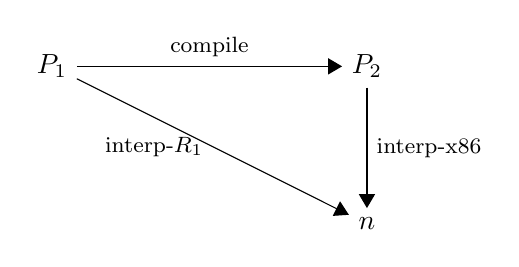
\begin{tikzpicture}[baseline=(current  bounding  box.center)]
 \node (p1) at (0,  0)   {$P_1$};
 \node (p2) at (4,  0)   {$P_2$};
 \node (o)  at (4, -2) {$n$};

 \path[->] (p1) edge [above] node {\footnotesize compile} (p2);
 \path[->] (p1) edge [left]  node {\footnotesize interp-$R_1$} (o);
 \path[->] (p2) edge [right] node {\footnotesize interp-x86} (o);
\end{tikzpicture}
\]
In the next section we introduce enough of the x86 assembly
language to compile $R_1$.

\section{The x86 Assembly Language}
\label{sec:x86}

An x86 program is a sequence of instructions. The instructions may
refer to integer constants (called \emph{immediate values}), variables
called \emph{registers}, and instructions may load and store values
into \emph{memory}.  Memory is a mapping of 64-bit addresses to 64-bit
values. Figure~\ref{fig:x86-a} defines the syntax for the subset of
the x86 assembly language needed for this chapter.  (We use the
AT\&T syntax expected by the GNU assembler inside \key{gcc}.)

\begin{figure}[tbp]
\fbox{
\begin{minipage}{0.96\textwidth}
\[
\begin{array}{lcl}
\Reg &::=& \key{rsp} \mid \key{rbp} \mid \key{rax} \mid \key{rbx} \mid \key{rcx}
              \mid \key{rdx} \mid \key{rsi} \mid \key{rdi} \mid \\
              && \key{r8} \mid \key{r9} \mid \key{r10}
              \mid \key{r11} \mid \key{r12} \mid \key{r13}
              \mid \key{r14} \mid \key{r15} \\
\Arg &::=&  \key{\$}\Int \mid \key{\%}\Reg \mid \Int(\key{\%}\Reg) \\ 
\Instr &::=& \key{addq} \; \Arg, \Arg \mid 
      \key{subq} \; \Arg, \Arg \mid 
%      \key{imulq} \; \Arg,\Arg \mid 
      \key{negq} \; \Arg \mid \key{movq} \; \Arg, \Arg \mid \\
  &&  \key{callq} \; \mathit{label} \mid
      \key{pushq}\;\Arg \mid \key{popq}\;\Arg \mid \key{retq} \\
\Prog &::= & \key{.globl main}\\
      &    & \key{main:} \; \Instr^{+}
\end{array}
\]
\end{minipage}
}
\caption{A subset of the x86 assembly language (AT\&T syntax).}
\label{fig:x86-a}
\end{figure}

An immediate value is written using the notation \key{\$}$n$ where $n$
is an integer. 
%
A register is written with a \key{\%} followed by the register name,
such as \key{\%rax}.
%
An access to memory is specified using the syntax $n(\key{\%}r)$,
which reads register $r$ and then offsets the address by $n$ bytes
(8 bits). The address is then used to either load or store to memory
depending on whether it occurs as a source or destination argument of
an instruction.

An arithmetic instruction, such as $\key{addq}\,s,\,d$, reads from the
source $s$ and destination $d$, applies the arithmetic operation, then
writes the result in $d$.
%
The move instruction, $\key{movq}\,s\,d$ reads from $s$ and stores the
result in $d$. 
%
The $\key{callq}\,\mathit{label}$ instruction executes the procedure
specified by the label.

Figure~\ref{fig:p0-x86} depicts an x86 program that is equivalent
to \code{(+ 10 32)}. The \key{globl} directive says that the
\key{main} procedure is externally visible, which is necessary so
that the operating system can call it. The label \key{main:}
indicates the beginning of the \key{main} procedure which is where
the operating system starts executing this program.  The instruction
\lstinline{movq $10, %rax} puts $10$ into register \key{rax}. The
following instruction \lstinline{addq $32, %rax} adds $32$ to the
$10$ in \key{rax} and puts the result, $42$, back into
\key{rax}. The instruction \lstinline{movq %rax, %rdi} moves the value 
in \key{rax} into another register, \key{rdi}, and 
\lstinline{callq print_int} calls the external function \code{print\_int}, which
prints the value in \key{rdi}.
The instruction \key{retq} finishes the \key{main}
function by returning the integer in \key{rax} to the
operating system.


%\begin{wrapfigure}{r}{2.25in}
\begin{figure}[tbp]
\begin{lstlisting}
	.globl main
main:
	movq	$10, %rax
	addq	$32, %rax
	movq	%rax, %rdi
	callq	print_int
	retq
\end{lstlisting}
\caption{An x86 program equivalent to $\BINOP{+}{10}{32}$.}
\label{fig:p0-x86}
%\end{wrapfigure}
\end{figure}
%% \marginpar{Consider using italics for the texts in these figures.
%%   It can get confusing to differentiate them from the main text.}
%% It looks pretty ugly in italics.-Jeremy

Unfortunately, x86 varies in a couple ways depending on what
operating system it is assembled in. The code examples shown here are
correct on the Unix platform, but when assembled on Mac OS X, labels
like \key{main} must be prefixed with an underscore.  So the correct
output for the above program on Mac would begin with:
\begin{lstlisting}
	.globl _main
_main:
	...
\end{lstlisting}

The next example exhibits the use of memory.  Figure~\ref{fig:p1-x86}
lists an x86 program that is equivalent to $\BINOP{+}{52}{
  \UNIOP{-}{10} }$. To understand how this x86 program works, we
need to explain a region of memory called the \emph{procedure call
  stack} (or \emph{stack} for short). The stack consists of a separate
\emph{frame} for each procedure call. The memory layout for an
individual frame is shown in Figure~\ref{fig:frame}.  The register
\key{rsp} is called the \emph{stack pointer} and points to the item at
the top of the stack. The stack grows downward in memory, so we
increase the size of the stack by subtracting from the stack
pointer. The frame size is required to be a multiple of 16 bytes. The
register \key{rbp} is the \emph{base pointer} which serves two
purposes: 1) it saves the location of the stack pointer for the
procedure that called the current one and 2) it is used to access
variables associated with the current procedure. We number the
variables from $1$ to $n$. Variable $1$ is stored at address
$-8\key{(\%rbp)}$, variable $2$ at $-16\key{(\%rbp)}$, etc.

%\begin{wrapfigure}{r}{2.1in}
\begin{figure}[tbp]
\begin{lstlisting}
	.globl main
main:
	pushq	%rbp
	movq	%rsp, %rbp
	subq	$16, %rsp

	movq	$10, -8(%rbp)
	negq	-8(%rbp)
	movq	$52, %rax
	addq	-8(%rbp), %rax

	movq	%rax, %rdi
	callq	print_int
	addq	$16, %rsp
	popq	%rbp
	retq
\end{lstlisting}
\caption{An x86 program equivalent to $\BINOP{+}{52}{\UNIOP{-}{10} }$.}
\label{fig:p1-x86}
\end{figure}
%\end{wrapfigure}


\begin{figure}[tbp]
\centering
\begin{tabular}{|r|l|} \hline
Position & Contents \\ \hline
8(\key{\%rbp}) & return address \\
0(\key{\%rbp}) & old \key{rbp} \\
-8(\key{\%rbp}) & variable $1$ \\
-16(\key{\%rbp}) & variable $2$ \\
 \ldots  & \ldots \\
0(\key{\%rsp}) & variable $n$\\ \hline
\end{tabular}

\caption{Memory layout of a frame.}
\label{fig:frame}
\end{figure}

Getting back to the program in Figure~\ref{fig:p1-x86}, the first
three instructions are the typical \emph{prelude} for a procedure.
The instruction \key{pushq \%rbp} saves the base pointer for the
procedure that called the current one onto the stack and subtracts $8$
from the stack pointer. The second instruction \key{movq \%rsp, \%rbp}
changes the base pointer to the top of the stack. The instruction
\key{subq \$16, \%rsp} moves the stack pointer down to make enough
room for storing variables.  This program just needs one variable ($8$
bytes) but because the frame size is required to be a multiple of 16
bytes, it rounds to 16 bytes.

The next four instructions carry out the work of computing
$\BINOP{+}{52}{\UNIOP{-}{10} }$. The first instruction \key{movq \$10,
  -8(\%rbp)} stores $10$ in variable $1$. The instruction \key{negq
  -8(\%rbp)} changes variable $1$ to $-10$. The \key{movq \$52, \%rax}
places $52$ in the register \key{rax} and \key{addq -8(\%rbp), \%rax}
adds the contents of variable $1$ to \key{rax}, at which point
\key{rax} contains $42$.

The last five instructions are the typical \emph{conclusion} of a
procedure. The first two print the final result of the program. The
latter three are necessary to get the state of the machine back to
where it was before the current procedure was called.  The \key{addq
  \$16, \%rsp} instruction moves the stack pointer back to point at
the old base pointer. The amount added here needs to match the amount
that was subtracted in the prelude of the procedure.  Then \key{popq
  \%rbp} returns the old base pointer to \key{rbp} and adds $8$ to the
stack pointer.  The \key{retq} instruction jumps back to the procedure
that called this one and subtracts 8 from the stack pointer.

The compiler will need a convenient representation for manipulating
x86 programs, so we define an abstract syntax for x86 in
Figure~\ref{fig:x86-ast-a}. The $\Int$ field of the \key{program} AST
node is number of bytes of stack space needed for variables in the
program. (Some of the intermediate languages will store other
information in that location for the purposes of communicating
auxiliary data from one step of the compiler to the next. )
%% \marginpar{Consider mentioning PseudoX86, since I think that's what
%%   you actually are referring to.}
%% Not here. PseudoX86 is the language with variables and
%% instructions that don't obey the x86 rules. -Jeremy

\begin{figure}[tbp]
\fbox{
\begin{minipage}{0.96\textwidth}
\[
\begin{array}{lcl}
\Arg &::=&  \INT{\Int} \mid \REG{\itm{register}}
    \mid \STACKLOC{\Int} \\ 
\Instr &::=& (\key{addq} \; \Arg\; \Arg) \mid 
             (\key{subq} \; \Arg\; \Arg) \mid 
%             (\key{imulq} \; \Arg\;\Arg) \mid 
             (\key{negq} \; \Arg) \mid (\key{movq} \; \Arg\; \Arg) \\
      &\mid& (\key{callq} \; \mathit{label}) \mid
             (\key{pushq}\;\Arg) \mid 
             (\key{popq}\;\Arg) \mid 
             (\key{retq}) \\
x86_0 &::= & (\key{program} \;\Int \; \Instr^{+})
\end{array}
\]
\end{minipage}
}
\caption{Abstract syntax for x86 assembly.}
\label{fig:x86-ast-a}
\end{figure}
%% \marginpar{I think this is PseudoX86, not x86.}

\section{Planning the trip from $R_1$ to x86}
\label{sec:plan-s0-x86}

To compile one language to another it helps to focus on the
differences between the two languages. It is these differences that
the compiler will need to bridge. What are the differences between
$R_1$ and x86 assembly? Here we list some of the most important the
differences.

\begin{enumerate}
\item x86 arithmetic instructions typically take two arguments and
  update the second argument in place. In contrast, $R_1$ arithmetic
  operations only read their arguments and produce a new value.

\item An argument to an $R_1$ operator can be any expression, whereas
  x86 instructions restrict their arguments to integers, registers,
  and memory locations.

\item An $R_1$ program can have any number of variables whereas x86
  has only 16 registers.

\item Variables in $R_1$ can overshadow other variables with the same
  name. The registers and memory locations of x86 all have unique
  names.
\end{enumerate}

We ease the challenge of compiling from $R_1$ to x86 by breaking down
the problem into several steps, dealing with the above differences one
at a time. The main question then becomes: in what order do we tackle
these differences? This is often one of the most challenging questions
that a compiler writer must answer because some orderings may be much
more difficult to implement than others. It is difficult to know ahead
of time which orders will be better so often some trial-and-error is
involved. However, we can try to plan ahead and choose the orderings
based on this planning.

For example, to handle difference \#2 (nested expressions), we shall
introduce new variables and pull apart the nested expressions into a
sequence of assignment statements.  To deal with difference \#3 we
will be replacing variables with registers and/or stack
locations. Thus, it makes sense to deal with \#2 before \#3 so that
\#3 can replace both the original variables and the new ones. Next,
consider where \#1 should fit in. Because it has to do with the format
of x86 instructions, it makes more sense after we have flattened the
nested expressions (\#2). Finally, when should we deal with \#4
(variable overshadowing)?  We shall solve this problem by renaming
variables to make sure they have unique names. Recall that our plan
for \#2 involves moving nested expressions, which could be problematic
if it changes the shadowing of variables. However, if we deal with \#4
first, then it will not be an issue.  Thus, we arrive at the following
ordering.
\[
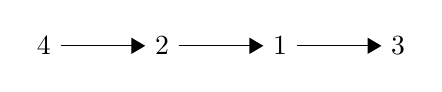
\begin{tikzpicture}[baseline=(current  bounding  box.center)]
\foreach \i/\p in {4/1,2/2,1/3,3/4}
{ 
  \node (\i) at (\p*1.5,0) {$\i$};
}
\foreach \x/\y in {4/2,2/1,1/3}
{
  \draw[->] (\x) to (\y);
}
\end{tikzpicture}
\]
We further simplify the translation from $R_1$ to x86 by identifying
an intermediate language named $C_0$, roughly half-way between $R_1$
and x86, to provide a rest stop along the way. We name the language
$C_0$ because it is vaguely similar to the $C$
language~\citep{Kernighan:1988nx}. The differences \#4 and \#1,
regarding variables and nested expressions, will be handled by two
steps, \key{uniquify} and \key{flatten}, which bring us to
$C_0$.
\[
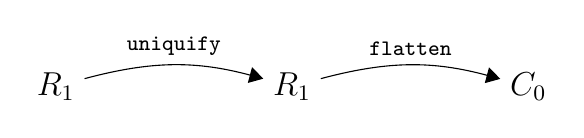
\begin{tikzpicture}[baseline=(current  bounding  box.center)]
\foreach \i/\p in {R_1/1,R_1/2,C_0/3}
{ 
  \node (\p) at (\p*3,0) {\large $\i$};
}
\foreach \x/\y/\lbl in {1/2/uniquify,2/3/flatten}
{
 \path[->,bend left=15] (\x) edge [above] node {\ttfamily\footnotesize \lbl} (\y);
}
\end{tikzpicture}
\]
Each of these steps in the compiler is implemented by a function,
typically a structurally recursive function that translates an input
AST into an output AST. We refer to such a function as a \emph{pass}
because it makes a pass over, i.e. it traverses the entire AST.

The syntax for $C_0$ is defined in Figure~\ref{fig:c0-syntax}.  The
$C_0$ language supports the same operators as $R_1$ but the arguments
of operators are now restricted to just variables and integers. The
\key{let} construct of $R_1$ is replaced by an assignment statement
and there is a \key{return} construct to specify the return value of
the program. A program consists of a sequence of statements that
include at least one \key{return} statement. Each program is also
annotated with a list of variables (viz. {\tt (var*)}). At the start
of the program, these variables are uninitialized (they contain garbage)
and each variable becomes initialized on its first assignment. All of
the variables used in the program must be present in this list.

\begin{figure}[tbp]
\fbox{
\begin{minipage}{0.96\textwidth}
\[
\begin{array}{lcl}
\Arg &::=& \Int \mid \Var \\
\Exp &::=& \Arg \mid (\key{read}) \mid (\key{-}\;\Arg) \mid (\key{+} \; \Arg\;\Arg)\\
\Stmt &::=& \ASSIGN{\Var}{\Exp} \mid \RETURN{\Arg} \\
C_0 & ::= & (\key{program}\;(\Var^{*})\;\Stmt^{+})
\end{array}
\]
\end{minipage}
}
\caption{The $C_0$ intermediate language.}
\label{fig:c0-syntax}
\end{figure}

To get from $C_0$ to x86 assembly it remains for us to handle
difference \#1 (the format of instructions) and difference \#3
(variables versus registers). These two differences are intertwined,
creating a bit of a Gordian Knot. To handle difference \#3, we need to
map some variables to registers (there are only 16 registers) and the
remaining variables to locations on the stack (which is unbounded). To
make good decisions regarding this mapping, we need the program to be
close to its final form (in x86 assembly) so we know exactly when
which variables are used. After all, variables that are used in
disjoint parts of the program can be assigned to the same register.
However, our choice of x86 instructions depends on whether the
variables are mapped to registers or stack locations, so we have a
circular dependency. We cut this knot by doing an optimistic selection
of instructions in the \key{select-instructions} pass, followed by the
\key{assign-homes} pass to map variables to registers or stack
locations, and conclude by finalizing the instruction selection in the
\key{patch-instructions} pass.
\[
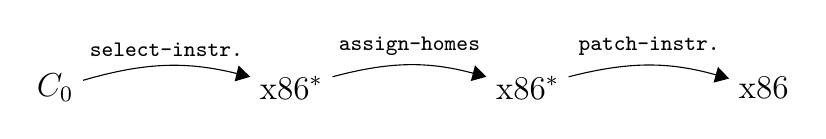
\begin{tikzpicture}[baseline=(current  bounding  box.center)]
\node (1) at (0,0)  {\large $C_0$};
\node (2) at (3,0)  {\large $\text{x86}^{*}$};
\node (3) at (6,0)  {\large $\text{x86}^{*}$};
\node (4) at (9,0) {\large $\text{x86}$};

\path[->,bend left=15] (1) edge [above] node {\ttfamily\footnotesize select-instr.} (2);
\path[->,bend left=15] (2) edge [above] node {\ttfamily\footnotesize assign-homes} (3);
\path[->,bend left=15] (3) edge [above] node {\ttfamily\footnotesize patch-instr.} (4);
\end{tikzpicture}
\]

The \key{select-instructions} pass is optimistic in the sense that it
treats variables as if they were all mapped to registers. The
\key{select-instructions} pass generates a program that consists of
x86 instructions but that still uses variables, so it is an
intermediate language that is technically different than x86, which
explains the asterisks in the diagram above.

In this Chapter we shall take the easy road to implementing
\key{assign-homes} and simply map all variables to stack locations.
The topic of Chapter~\ref{ch:register-allocation} is implementing a
smarter approach in which we make a best-effort to map variables to
registers, resorting to the stack only when necessary.

%% \marginpar{\scriptsize I'm confused: shouldn't `select instructions' do this?
%% After all, that selects the x86 instructions. Even if it is separate,
%% if we perform `patching' before register allocation, we aren't forced to rely on
%% \key{rax} as much. This can ultimately make a more-performant result. --
%% Cam}


Once variables have been assigned to their homes, we can finalize the
instruction selection by dealing with an idiosyncrasy of x86
assembly. Many x86 instructions have two arguments but only one of the
arguments may be a memory reference (and the stack is a part of
memory).  Because some variables may get mapped to stack locations,
some of our generated instructions may violate this restriction.  The
purpose of the \key{patch-instructions} pass is to fix this problem by
replacing every violating instruction with a short sequence of
instructions that use the \key{rax} register. Once we have implemented
a good register allocator (Chapter~\ref{ch:register-allocation}), the
need to patch instructions will be relatively rare.


\section{Uniquify Variables}
\label{sec:uniquify-s0}

The purpose of this pass is to make sure that each \key{let} uses a
unique variable name. For example, the \code{uniquify} pass should
translate the program on the left into the program on the right. \\
\begin{tabular}{lll}
\begin{minipage}{0.4\textwidth}
\begin{lstlisting}
 (program
   (let ([x 32])
     (+ (let ([x 10]) x) x)))
\end{lstlisting}
\end{minipage}
&
$\Rightarrow$
&
\begin{minipage}{0.4\textwidth}
\begin{lstlisting}
(program
  (let ([x.1 32])
    (+ (let ([x.2 10]) x.2) x.1)))
\end{lstlisting}
\end{minipage}
\end{tabular} \\
%
The following is another example translation, this time of a program
with a \key{let} nested inside the initializing expression of another
\key{let}.\\
\begin{tabular}{lll}
\begin{minipage}{0.4\textwidth}
\begin{lstlisting}
(program
  (let ([x (let ([x 4])
             (+ x 1))])
    (+ x 2)))
\end{lstlisting}
\end{minipage}
&
$\Rightarrow$
&
\begin{minipage}{0.4\textwidth}
\begin{lstlisting}
(program
  (let ([x.2 (let ([x.1 4])
               (+ x.1 1))])
    (+ x.2 2)))
\end{lstlisting}
\end{minipage}
\end{tabular}

We recommend implementing \code{uniquify} as a structurally recursive
function that mostly copies the input program. However, when
encountering a \key{let}, it should generate a unique name for the
variable (the Racket function \code{gensym} is handy for this) and
associate the old name with the new unique name in an association
list. The \code{uniquify} function will need to access this
association list when it gets to a variable reference, so we add
another parameter to \code{uniquify} for the association list. It is
quite common for a compiler pass to need a map to store extra
information about variables. Such maps are often called \emph{symbol
  tables}.

The skeleton of the \code{uniquify} function is shown in
Figure~\ref{fig:uniquify-s0}.  The function is curried so that it is
convenient to partially apply it to an association list and then apply
it to different expressions, as in the last clause for primitive
operations in Figure~\ref{fig:uniquify-s0}. In the last \key{match}
clause for the primitive operators, note the use of the comma-@
operator to splice a list of S-expressions into an enclosing
S-expression.

\begin{exercise}
\normalfont % I don't like the italics for exercises. -Jeremy

Complete the \code{uniquify} pass by filling in the blanks, that is,
implement the clauses for variables and for the \key{let} construct.
\end{exercise}

\begin{figure}[tbp]
\begin{lstlisting}
   (define uniquify
     (lambda (alist)
       (lambda (e)
         (match e
           [(? symbol?) ___]
           [(? integer?) e]
           [`(let ([,x ,e]) ,body) ___]
           [`(program ,e)
            `(program ,((uniquify alist) e))]
           [`(,op ,es ...)
            `(,op ,@(map (uniquify alist) es))]
           ))))
\end{lstlisting}
\caption{Skeleton for the \key{uniquify} pass.}
\label{fig:uniquify-s0}
\end{figure}

\begin{exercise}
\normalfont % I don't like the italics for exercises. -Jeremy 

Test your \key{uniquify} pass by creating five example $R_1$ programs
and checking whether the output programs produce the same result as
the input programs. The $R_1$ programs should be designed to test the
most interesting parts of the \key{uniquify} pass, that is, the
programs should include \key{let} constructs, variables, and variables
that overshadow each other.  The five programs should be in a
subdirectory named \key{tests} and they should have the same file name
except for a different integer at the end of the name, followed by the
ending \key{.rkt}.  Use the \key{interp-tests} function
(Appendix~\ref{appendix:utilities}) from \key{utilities.rkt} to test
your \key{uniquify} pass on the example programs.

\end{exercise}


\section{Flatten Expressions}
\label{sec:flatten-r1}

The \code{flatten} pass will transform $R_1$ programs into $C_0$
programs. In particular, the purpose of the \code{flatten} pass is to
get rid of nested expressions, such as the \code{(- 10)} in the program
below. This can be accomplished by introducing a new variable,
assigning the nested expression to the new variable, and then using
the new variable in place of the nested expressions, as shown in the
output of \code{flatten} on the right.\\
\begin{tabular}{lll}
\begin{minipage}{0.4\textwidth}
\begin{lstlisting}
 (program
   (+ 52 (- 10)))
\end{lstlisting}
\end{minipage}
&
$\Rightarrow$
&
\begin{minipage}{0.4\textwidth}
\begin{lstlisting}
(program (tmp.1 tmp.2)
  (assign tmp.1 (- 10))
  (assign tmp.2 (+ 52 tmp.1))
  (return tmp.2))
\end{lstlisting}
\end{minipage}
\end{tabular}

The clause of \code{flatten} for \key{let} is straightforward to
implement as it just requires the generation of an assignment
statement for the \key{let}-bound variable. The following shows the
result of \code{flatten} for a \key{let}. \\
\begin{tabular}{lll}
\begin{minipage}{0.4\textwidth}
\begin{lstlisting}
 (program
   (let ([x (+ (- 10) 11)])
     (+ x 41)))
\end{lstlisting}
\end{minipage}
&
$\Rightarrow$
&
\begin{minipage}{0.4\textwidth}
\begin{lstlisting}
(program (tmp.1 x tmp.2)
  (assign tmp.1 (- 10))
  (assign x (+ tmp.1 11))
  (assign tmp.2 (+ x 41))
  (return tmp.2))
\end{lstlisting}
\end{minipage}
\end{tabular}

We recommend implementing \key{flatten} as a structurally recursive
function that returns two things, 1) the newly flattened expression,
and 2) a list of assignment statements, one for each of the new
variables introduced during the flattening the expression.  The newly
flattened expression should be an $\Arg$ in the $C_0$ syntax
(Figure~\ref{fig:c0-syntax}), that is, it should be an integer or a
variable. You can return multiple things from a function using the
\key{values} form and you can receive multiple things from a function
call using the \key{define-values} form. If you are not familiar with
these constructs, the Racket documentation will be of help. Also, the
\key{map2} function (Appendix~\ref{appendix:utilities}) is useful for
applying a function to each element of a list, in the case where the
function returns two values. The result of \key{map2} is two lists.

The clause of \key{flatten} for the \key{program} node needs to
recursively flatten the body of the program and the newly flattened
expression should be placed in a \key{return} statement.  The
\key{flatten} pass should also compute the list of variables used in
the program.  I recommend traversing the statements in the body of the
program (after it has been flattened) and collect all variables that
appear on the left-hand-side of an assignment. Note that each variable
should only occur once in the list of variables that you place in the
\key{program} form.

Take special care for programs such as the following that initialize
variables with integers or other variables. It should be translated
to the program on the right \\
\begin{tabular}{lll}
\begin{minipage}{0.4\textwidth}
\begin{lstlisting}
  (let ([a 42])
    (let ([b a])
      b))
\end{lstlisting}
\end{minipage}
&
$\Rightarrow$
&
\begin{minipage}{0.4\textwidth}
\begin{lstlisting}
(program (a b)
  (assign a 42)
  (assign b a)
  (return b))
\end{lstlisting}
\end{minipage}
\end{tabular} \\
and not to the following, which could result from a naive
implementation of \key{flatten}.
\begin{lstlisting}
   (program (tmp.1 a tmp.2 b)
     (assign tmp.1 42)
     (assign a tmp.1)
     (assign tmp.2 a)
     (assign b tmp.2)
     (return b))
\end{lstlisting}

\begin{exercise}
\normalfont
Implement the \key{flatten} pass and test it on all of the example
programs that you created to test the \key{uniquify} pass and create
three new example programs that are designed to exercise all of the
interesting code in the \key{flatten} pass. Use the \key{interp-tests}
function (Appendix~\ref{appendix:utilities}) from \key{utilities.rkt} to
test your passes on the example programs.
\end{exercise}


\section{Select Instructions}
\label{sec:select-s0}

In the \key{select-instructions} pass we begin the work of translating
from $C_0$ to x86. The target language of this pass is a pseudo-x86
language that still uses variables, so we add an AST node of the form
$\VAR{\itm{var}}$ to the x86 abstract syntax. Also, the \key{program}
form should still list the variables (similar to $C_0$):
\[
  (\key{program}\;(\Var^{*})\;\Instr^{+})
\]
The \key{select-instructions} pass deals with the differing format of
arithmetic operations. For example, in $C_0$ an addition operation can
take the form below.  To translate to x86, we need to use the
\key{addq} instruction which does an in-place update. So we must first
move \code{10} to \code{x}. \\
\begin{tabular}{lll}
\begin{minipage}{0.4\textwidth}
\begin{lstlisting}
 (assign x (+ 10 32))
\end{lstlisting}
\end{minipage}
&
$\Rightarrow$
&
\begin{minipage}{0.4\textwidth}
\begin{lstlisting}
   (movq (int 10) (var x))
   (addq (int 32) (var x))
\end{lstlisting}
\end{minipage}
\end{tabular} \\

There are some cases that require special care to avoid generating
needlessly complicated code. If one of the arguments is the same as
the left-hand side of the assignment, then there is no need for the
extra move instruction.  For example, the following assignment
statement can be translated into a single \key{addq} instruction.\\
\begin{tabular}{lll}
\begin{minipage}{0.4\textwidth}
\begin{lstlisting}
 (assign x (+ 10 x))
\end{lstlisting}
\end{minipage}
&
$\Rightarrow$
&
\begin{minipage}{0.4\textwidth}
\begin{lstlisting}
(addq (int 10) (var x))
\end{lstlisting}
\end{minipage}
\end{tabular} \\

The \key{read} operation does not have a direct counterpart in x86
assembly, so we have instead implemented this functionality in the C
language, with the function \code{read\_int} in the file
\code{runtime.c}. In general, we refer to all of the functionality in
this file as the \emph{runtime system}, or simply the \emph{runtime}
for short. When compiling your generated x86 assembly code, you
will need to compile \code{runtime.c} to \code{runtime.o} (an ``object
file'', using \code{gcc} option \code{-c}) and link it into the final
executable. For our purposes of code generation, all you need to do is
translate an assignment of \key{read} to some variable $\itm{lhs}$
(for left-hand side) into a call to the \code{read\_int} function
followed by a move from \code{rax} to the left-hand side.  The move
from \code{rax} is needed because the return value from
\code{read\_int} goes into \code{rax}, as is the case in general.  \\
\begin{tabular}{lll}
\begin{minipage}{0.4\textwidth}
\begin{lstlisting}
 (assign |$\itm{lhs}$| (read))
\end{lstlisting}
\end{minipage}
&
$\Rightarrow$
&
\begin{minipage}{0.4\textwidth}
\begin{lstlisting}
(callq read_int)
(movq (reg rax) (var |$\itm{lhs}$|))
\end{lstlisting}
\end{minipage}
\end{tabular} \\

Regarding the \RETURN{\Arg} statement of $C_0$, we recommend treating it
as an assignment to the \key{rax} register and let the procedure
conclusion handle the transfer of control back to the calling
procedure.

\begin{exercise}
\normalfont
Implement the \key{select-instructions} pass and test it on all of the
example programs that you created for the previous passes and create
three new example programs that are designed to exercise all of the
interesting code in this pass. Use the \key{interp-tests} function
(Appendix~\ref{appendix:utilities}) from \key{utilities.rkt} to test
your passes on the example programs.
\end{exercise}

\section{Assign Homes}
\label{sec:assign-s0}

As discussed in Section~\ref{sec:plan-s0-x86}, the
\key{assign-homes} pass places all of the variables on the stack.
Consider again the example $R_1$ program \code{(+ 52 (- 10))},
which after \key{select-instructions} looks like the following.
\begin{lstlisting}
   (movq (int 10) (var x))
   (negq (var x))
   (movq (int 52) (reg rax))
   (addq (var x) (reg rax))
\end{lstlisting}
The one and only variable \code{x} is assigned to stack location
\code{-8(\%rbp)}, so the \code{assign-homes} pass translates the
above to
\begin{lstlisting}
   (movq (int 10) (stack -8))
   (negq (stack -8))
   (movq (int 52) (reg rax))
   (addq (stack -8) (reg rax))
\end{lstlisting}

In the process of assigning stack locations to variables, it is
convenient to compute and store the size of the frame in the first
field of the \key{program} node which will be needed later to generate
the procedure conclusion. 
\[
  (\key{program}\;\Int\;\Instr^{+})
\]
Some operating systems place restrictions on
the frame size. For example, Mac OS X requires the frame size to be a
multiple of 16 bytes.

\begin{exercise}
\normalfont Implement the \key{assign-homes} pass and test it on all
of the example programs that you created for the previous passes pass.
I recommend that \key{assign-homes} take an extra parameter that is a
mapping of variable names to homes (stack locations for now).  Use the
\key{interp-tests} function (Appendix~\ref{appendix:utilities}) from
\key{utilities.rkt} to test your passes on the example programs.
\end{exercise}

\section{Patch Instructions}
\label{sec:patch-s0}

The purpose of this pass is to make sure that each instruction adheres
to the restrictions regarding which arguments can be memory
references. For most instructions, the rule is that at most one
argument may be a memory reference.

Consider again the following example.
\begin{lstlisting}
   (let ([a 42])
     (let ([b a])
       b))
\end{lstlisting}
After \key{assign-homes} pass, the above has been translated to
\begin{lstlisting}
   (movq (int 42) (stack -8))
   (movq (stack -8) (stack -16))
   (movq (stack -16) (reg rax))
\end{lstlisting}
The second \key{movq} instruction is problematic because both arguments
are stack locations. We suggest fixing this problem by moving from the
source to \key{rax} and then from \key{rax} to the destination, as
follows.
\begin{lstlisting}
   (movq (int 42) (stack -8))
   (movq (stack -8) (reg rax))
   (movq (reg rax) (stack -16))
   (movq (stack -16) (reg rax))
\end{lstlisting}

\begin{exercise}
\normalfont
Implement the \key{patch-instructions} pass and test it on all of the
example programs that you created for the previous passes and create
three new example programs that are designed to exercise all of the
interesting code in this pass. Use the \key{interp-tests} function
(Appendix~\ref{appendix:utilities}) from \key{utilities.rkt} to test
your passes on the example programs.
\end{exercise}


\section{Print x86}
\label{sec:print-x86}

The last step of the compiler from $R_1$ to x86 is to convert the
x86 AST (defined in Figure~\ref{fig:x86-ast-a}) to the string
representation (defined in Figure~\ref{fig:x86-a}). The Racket
\key{format} and \key{string-append} functions are useful in this
regard. The main work that this step needs to perform is to create the
\key{main} function and the standard instructions for its prelude
and conclusion, as shown in Figure~\ref{fig:p1-x86} of
Section~\ref{sec:x86}. You need to know the number of
stack-allocated variables, for which it is suggest that you compute in
the \key{assign-homes} pass (Section~\ref{sec:assign-s0}) and store in
the $\itm{info}$ field of the \key{program} node.

Your compiled code should print the result of the program's execution by using the
\code{print\_int} function provided in \code{runtime.c}. If your compiler has been implemented correctly so far, this final result should be stored in the \key{rax} register.
We'll talk more about
how to perform function calls with arguments in general later on, but
for now, make sure that your x86 printer includes the following code as part of the conclusion:

\begin{lstlisting}
    movq %rax, %rdi
    callq print_int
\end{lstlisting}

These lines move the value in \key{rax} into the \key{rdi} register, which
stores the first argument to be passed into \key{print\_int}.

If you want your program to run on Mac OS X, your code needs to
determine whether or not it is running on a Mac, and prefix
underscores to labels like \key{main}.  You can determine the platform
with the Racket call \code{(system-type 'os)}, which returns
\code{'macosx}, \code{'unix}, or \code{'windows}.  In addition to
placing underscores on \key{main}, you need to put them in front of
\key{callq} labels (so \code{callq print\_int} becomes \code{callq
  \_print\_int}).

\begin{exercise}
\normalfont Implement the \key{print-x86} pass and test it on all of
the example programs that you created for the previous passes. Use the
\key{compiler-tests} function (Appendix~\ref{appendix:utilities}) from
\key{utilities.rkt} to test your complete compiler on the example
programs. 
% The following is specific to P423/P523. -Jeremy
%Mac support is optional, but your compiler has to output
%valid code for Unix machines.
\end{exercise}

\begin{figure}[p]
\begin{tikzpicture}[baseline=(current  bounding  box.center)]
\node (R1) at (0,2)  {\large $R_1$};
\node (R1-2) at (3,2)  {\large $R_1$};
\node (C0-1) at (3,0)  {\large $C_0$};

\node (x86-2) at (3,-2)  {\large $\text{x86}^{*}$};
\node (x86-3) at (6,-2)  {\large $\text{x86}^{*}$};
\node (x86-4) at (9,-2) {\large $\text{x86}$};
\node (x86-5) at (12,-2) {\large $\text{x86}^{\dagger}$};

\path[->,bend left=15] (R1) edge [above] node {\ttfamily\footnotesize uniquify} (R1-2);
\path[->,bend left=15] (R1-2) edge [right] node {\ttfamily\footnotesize flatten} (C0-1);
\path[->,bend right=15] (C0-1) edge [left] node {\ttfamily\footnotesize select-instr.} (x86-2);
\path[->,bend left=15] (x86-2) edge [above] node {\ttfamily\footnotesize assign-homes} (x86-3);
\path[->,bend left=15] (x86-3) edge [above] node {\ttfamily\footnotesize patch-instr.} (x86-4);
\path[->,bend left=15] (x86-4) edge [above] node {\ttfamily\footnotesize print-x86} (x86-5);
\end{tikzpicture}

\caption{Overview of the passes for compiling $R_1$.  The x86$^{*}$
  language extends x86 with variables and looser rules regarding
  instruction arguments. The x86$^{\dagger}$ language is the concrete
  syntax (string) for x86.}
\label{fig:R1-passes}
\end{figure}


Figure~\ref{fig:R1-passes} provides an overview of all the compiler
passes described in this Chapter.



%%%%%%%%%%%%%%%%%%%%%%%%%%%%%%%%%%%%%%%%%%%%%%%%%%%%%%%%%%%%%%%%%%%%%%%%%%%%%%%%
\chapter{Register Allocation}
\label{ch:register-allocation}

In Chapter~\ref{ch:int-exp} we simplified the generation of x86
assembly by placing all variables on the stack. We can improve the
performance of the generated code considerably if we instead try to
place as many variables as possible into registers.  The CPU can
access a register in a single cycle, whereas accessing the stack can
take from several cycles (to go to cache) to hundreds of cycles (to go
to main memory).  Figure~\ref{fig:reg-eg} shows a program with four
variables that serves as a running example. We show the source program
and also the output of instruction selection. At that point the
program is almost x86 assembly but not quite; it still contains
variables instead of stack locations or registers.

\begin{figure}
\begin{minipage}{0.45\textwidth}
Source program:
\begin{lstlisting}
(program
  (let ([v 1])
  (let ([w 46])
  (let ([x (+ v 7)])
  (let ([y (+ 4 x)])
  (let ([z (+ x w)])
       (+ z (- y))))))))
\end{lstlisting}
\end{minipage}
\begin{minipage}{0.45\textwidth}
After instruction selection:
\begin{lstlisting}
(program (v w x y z t.1 t.2)
  (movq (int 1) (var v))
  (movq (int 46) (var w))
  (movq (var v) (var x))
  (addq (int 7) (var x))
  (movq (var x) (var y))
  (addq (int 4) (var y))
  (movq (var x) (var z))
  (addq (var w) (var z))
  (movq (var y) (var t.1))
  (negq (var t.1))
  (movq (var z) (var t.2))
  (addq (var t.1) (var t.2))
  (movq (var t.2) (reg rax)))
\end{lstlisting}
\end{minipage}
\caption{Running example for this chapter.}
\label{fig:reg-eg}
\end{figure}

The goal of register allocation is to fit as many variables into
registers as possible. It is often the case that we have more
variables than registers, so we cannot naively map each variable to a
register. Fortunately, it is also common for different variables to be
needed during different periods of time, and in such cases the
variables can be mapped to the same register.  Consider variables
\code{x} and \code{y} in Figure~\ref{fig:reg-eg}.  After the variable
\code{x} is moved to \code{z} it is no longer needed.  Variable
\code{y}, on the other hand, is used only after this point, so
\code{x} and \code{y} could share the same register. The topic of the
next section is how we compute where a variable is needed.


\section{Liveness Analysis}
\label{sec:liveness-analysis}

A variable is \emph{live} if the variable is used at some later point
in the program and there is not an intervening assignment to the
variable.
%
To understand the latter condition, consider the following code
fragment in which there are two writes to \code{b}. Are \code{a} and
\code{b} both live at the same time?
\begin{lstlisting}[numbers=left,numberstyle=\tiny]
   (movq (int 5) (var a))
   (movq (int 30) (var b))
   (movq (var a) (var c))
   (movq (int 10) (var b))
   (addq (var b) (var c))
\end{lstlisting}
The answer is no because the value \code{30} written to \code{b} on
line 2 is never used. The variable \code{b} is read on line 5 and
there is an intervening write to \code{b} on line 4, so the read on
line 5 receives the value written on line 4, not line 2.

The live variables can be computed by traversing the instruction
sequence back to front (i.e., backwards in execution order).  Let
$I_1,\ldots, I_n$ be the instruction sequence. We write
$L_{\mathsf{after}}(k)$ for the set of live variables after
instruction $I_k$ and $L_{\mathsf{before}}(k)$ for the set of live
variables before instruction $I_k$. The live variables after an
instruction are always the same as the live variables before the next
instruction.
\begin{equation*}
  L_{\mathsf{after}}(k) = L_{\mathsf{before}}(k+1)
\end{equation*}
To start things off, there are no live variables after the last
instruction, so 
\begin{equation*}
  L_{\mathsf{after}}(n) = \emptyset 
\end{equation*}
We then apply the following rule repeatedly, traversing the
instruction sequence back to front.
\begin{equation*}
  L_{\mathtt{before}}(k) = (L_{\mathtt{after}}(k) - W(k)) \cup R(k),
\end{equation*}
where $W(k)$ are the variables written to by instruction $I_k$ and
$R(k)$ are the variables read by instruction $I_k$.
Figure~\ref{fig:live-eg} shows the results of live variables analysis
for the running example, with each instruction aligned with its
$L_{\mathtt{after}}$ set to make the figure easy to read.


\begin{figure}[tbp]
\hspace{20pt}
\begin{minipage}{0.45\textwidth}
\begin{lstlisting}[numbers=left]
  (program (v w x y z t.1 t.2)
    (movq (int 1) (var v))
    (movq (int 46) (var w))
    (movq (var v) (var x))
    (addq (int 7) (var x))
    (movq (var x) (var y))
    (addq (int 4) (var y))
    (movq (var x) (var z))
    (addq (var w) (var z))
    (movq (var y) (var t.1))
    (negq (var t.1))
    (movq (var z) (var t.2))
    (addq (var t.1) (var t.2))
    (movq (var t.2) (reg rax)))
\end{lstlisting}
\end{minipage}
\vrule\hspace{10pt}
\begin{minipage}{0.45\textwidth}
\begin{lstlisting}

|$\{ v \}$|
|$\{ v, w \}$|
|$\{ w, x \}$|
|$\{ w, x \}$|
|$\{ w, x, y\}$|
|$\{ w, x, y \}$|
|$\{ w, y, z \}$|
|$\{ y, z \}$|
|$\{ t.1, z \}$|
|$\{ t.1, z \}$|
|$\{t.1,t.2\}$|
|$\{t.2\}$|
|$\{\}$|
\end{lstlisting}
\end{minipage}

\caption{The running example and its live-after sets.}
\label{fig:live-eg}
\end{figure}

\begin{exercise}\normalfont
Implement the compiler pass named \code{uncover-live} that computes
the live-after sets. We recommend storing the live-after sets (a list
of lists of variables) in the $\itm{info}$ field of the \key{program}
node alongside the list of variables as follows.
\begin{lstlisting}
   (program (|$\Var^{*}$| |$\itm{live{-}afters}$|) |$\Instr^{+}$|)
\end{lstlisting}
I recommend organizing your code to use a helper function that takes a
list of statements and an initial live-after set (typically empty) and
returns the list of statements and the list of live-after sets.  For
this chapter, returning the list of statements is unnecessary, as they
will be unchanged, but in Chapter~\ref{ch:bool-types} we introduce
\key{if} statements and will need to annotate them with the live-after
sets of the two branches.

I recommend creating helper functions to 1) compute the set of
variables that appear in an argument (of an instruction), 2) compute
the variables read by an instruction which corresponds to the $R$
function discussed above, and 3) the variables written by an
instruction which corresponds to $W$.
\end{exercise}

\section{Building the Interference Graph}

Based on the liveness analysis, we know where each variable is needed.
However, during register allocation, we need to answer questions of
the specific form: are variables $u$ and $v$ live at the same time?
(And therefore cannot be assigned to the same register.)  To make this
question easier to answer, we create an explicit data structure, an
\emph{interference graph}.  An interference graph is an undirected
graph that has an edge between two variables if they are live at the
same time, that is, if they interfere with each other.

The most obvious way to compute the interference graph is to look at
the set of live variables between each statement in the program, and
add an edge to the graph for every pair of variables in the same set.
This approach is less than ideal for two reasons. First, it can be
rather expensive because it takes $O(n^2)$ time to look at every pair
in a set of $n$ live variables. Second, there is a special case in
which two variables that are live at the same time do not actually
interfere with each other: when they both contain the same value
because we have assigned one to the other.

A better way to compute the interference graph is given by the
following.

\begin{itemize}
\item If instruction $I_k$ is a move: (\key{movq} $s$\, $d$), then add
  the edge $(d,v)$ for every $v \in L_{\mathsf{after}}(k)$ unless $v =
  d$ or $v = s$.

\item If instruction $I_k$ is not a move but some other arithmetic
  instruction such as (\key{addq} $s$\, $d$), then add the edge $(d,v)$
  for every $v \in L_{\mathsf{after}}(k)$ unless $v = d$.
  
\item If instruction $I_k$ is of the form (\key{callq}
  $\mathit{label}$), then add an edge $(r,v)$ for every caller-save
  register $r$ and every variable $v \in L_{\mathsf{after}}(k)$.
\end{itemize}

Working from the top to bottom of Figure~\ref{fig:live-eg}, we obtain
the following interference for the instruction at the specified line
number.
\begin{quote}
Line 2: no interference,\\
Line 3: $w$ interferes with $v$,\\
Line 4: $x$ interferes with $w$,\\
Line 5: $x$ interferes with $w$,\\
Line 6: $y$ interferes with $w$,\\
Line 7: $y$ interferes with $w$ and $x$,\\
Line 8: $z$ interferes with $w$ and $y$,\\
Line 9: $z$ interferes with $y$, \\
Line 10: $t.1$ interferes with $z$, \\
Line 11: $t.1$ interferes with $z$, \\
Line 12: $t.2$ interferes with $t.1$, \\
Line 13: no interference. \\
Line 14: no interference. 
\end{quote}
The resulting interference graph is shown in
Figure~\ref{fig:interfere}. 

\begin{figure}[tbp]
\large
\[
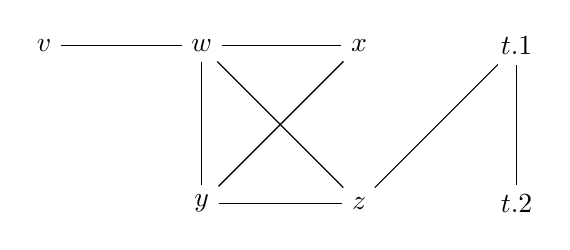
\begin{tikzpicture}[baseline=(current  bounding  box.center)]
\node (v) at (0,0)   {$v$};
\node (w) at (2,0)   {$w$};
\node (x) at (4,0)   {$x$};
\node (t1) at (6,0)   {$t.1$};
\node (y) at (2,-2)  {$y$};
\node (z) at (4,-2)  {$z$};
\node (t2) at (6,-2) {$t.2$};

\draw (v) to (w);
\foreach \i in {w,x,y} 
{
  \foreach \j in {w,x,y}
  { 
    \draw (\i) to (\j);
  }
}
\draw (z) to (w);
\draw (z) to (y);
\draw (t1) to (z);
\draw (t2) to (t1);
\end{tikzpicture}
\]
\caption{Interference graph for the running example.}
\label{fig:interfere}
\end{figure}

Our next concern is to choose a data structure for representing the
interference graph. There are many standard choices for how to
represent a graph: \emph{adjacency matrix}, \emph{adjacency list}, and
\emph{edge set}~\citep{Cormen:2001uq}. The right way to choose a data
structure is to study the algorithm that uses the data structure,
determine what operations need to be performed, and then choose the
data structure that provide the most efficient implementations of
those operations. Often times the choice of data structure can have an
affect on the time complexity of the algorithm, as it does here. If
you skim the next section, you will see that the register allocation
algorithm needs to ask the graph for all of its vertices and, given a
vertex, it needs to known all of the adjacent vertices. Thus, the
correct choice of graph representation is that of an adjacency
list. There are helper functions in \code{utilities.rkt} for
representing graphs using the adjacency list representation:
\code{make-graph}, \code{add-edge}, and \code{adjacent}
(Appendix~\ref{appendix:utilities}).  In particular, those functions
use a hash table to map each vertex to the set of adjacent vertices,
and the sets are represented using Racket's \key{set}, which is also a
hash table.

\begin{exercise}\normalfont
Implement the compiler pass named \code{build-interference} according
to the algorithm suggested above.  The output of this pass should
replace the live-after sets with the interference $\itm{graph}$ as
follows.
\begin{lstlisting}
   (program (|$\Var^{*}$| |$\itm{graph}$|) |$\Instr^{+}$|)
\end{lstlisting}

\end{exercise}

\section{Graph Coloring via Sudoku}

We now come to the main event, mapping variables to registers (or to
stack locations in the event that we run out of registers).  We need
to make sure not to map two variables to the same register if the two
variables interfere with each other.  In terms of the interference
graph, this means we cannot map adjacent nodes to the same register.
If we think of registers as colors, the register allocation problem
becomes the widely-studied graph coloring
problem~\citep{Balakrishnan:1996ve,Rosen:2002bh}.  

The reader may be more familiar with the graph coloring problem then he
or she realizes; the popular game of Sudoku is an instance of the
graph coloring problem. The following describes how to build a graph
out of an initial Sudoku board.
\begin{itemize}
\item There is one node in the graph for each Sudoku square.
\item There is an edge between two nodes if the corresponding squares
  are in the same row, in the same column, or if the squares are in
  the same $3\times 3$ region.
\item Choose nine colors to correspond to the numbers $1$ to $9$.
\item Based on the initial assignment of numbers to squares in the
  Sudoku board, assign the corresponding colors to the corresponding
  nodes in the graph.
\end{itemize}
If you can color the remaining nodes in the graph with the nine
colors, then you have also solved the corresponding game of Sudoku.
Figure~\ref{fig:sudoku-graph} shows an initial Sudoku game board and
the corresponding graph with colored vertices.

\begin{figure}[tbp]
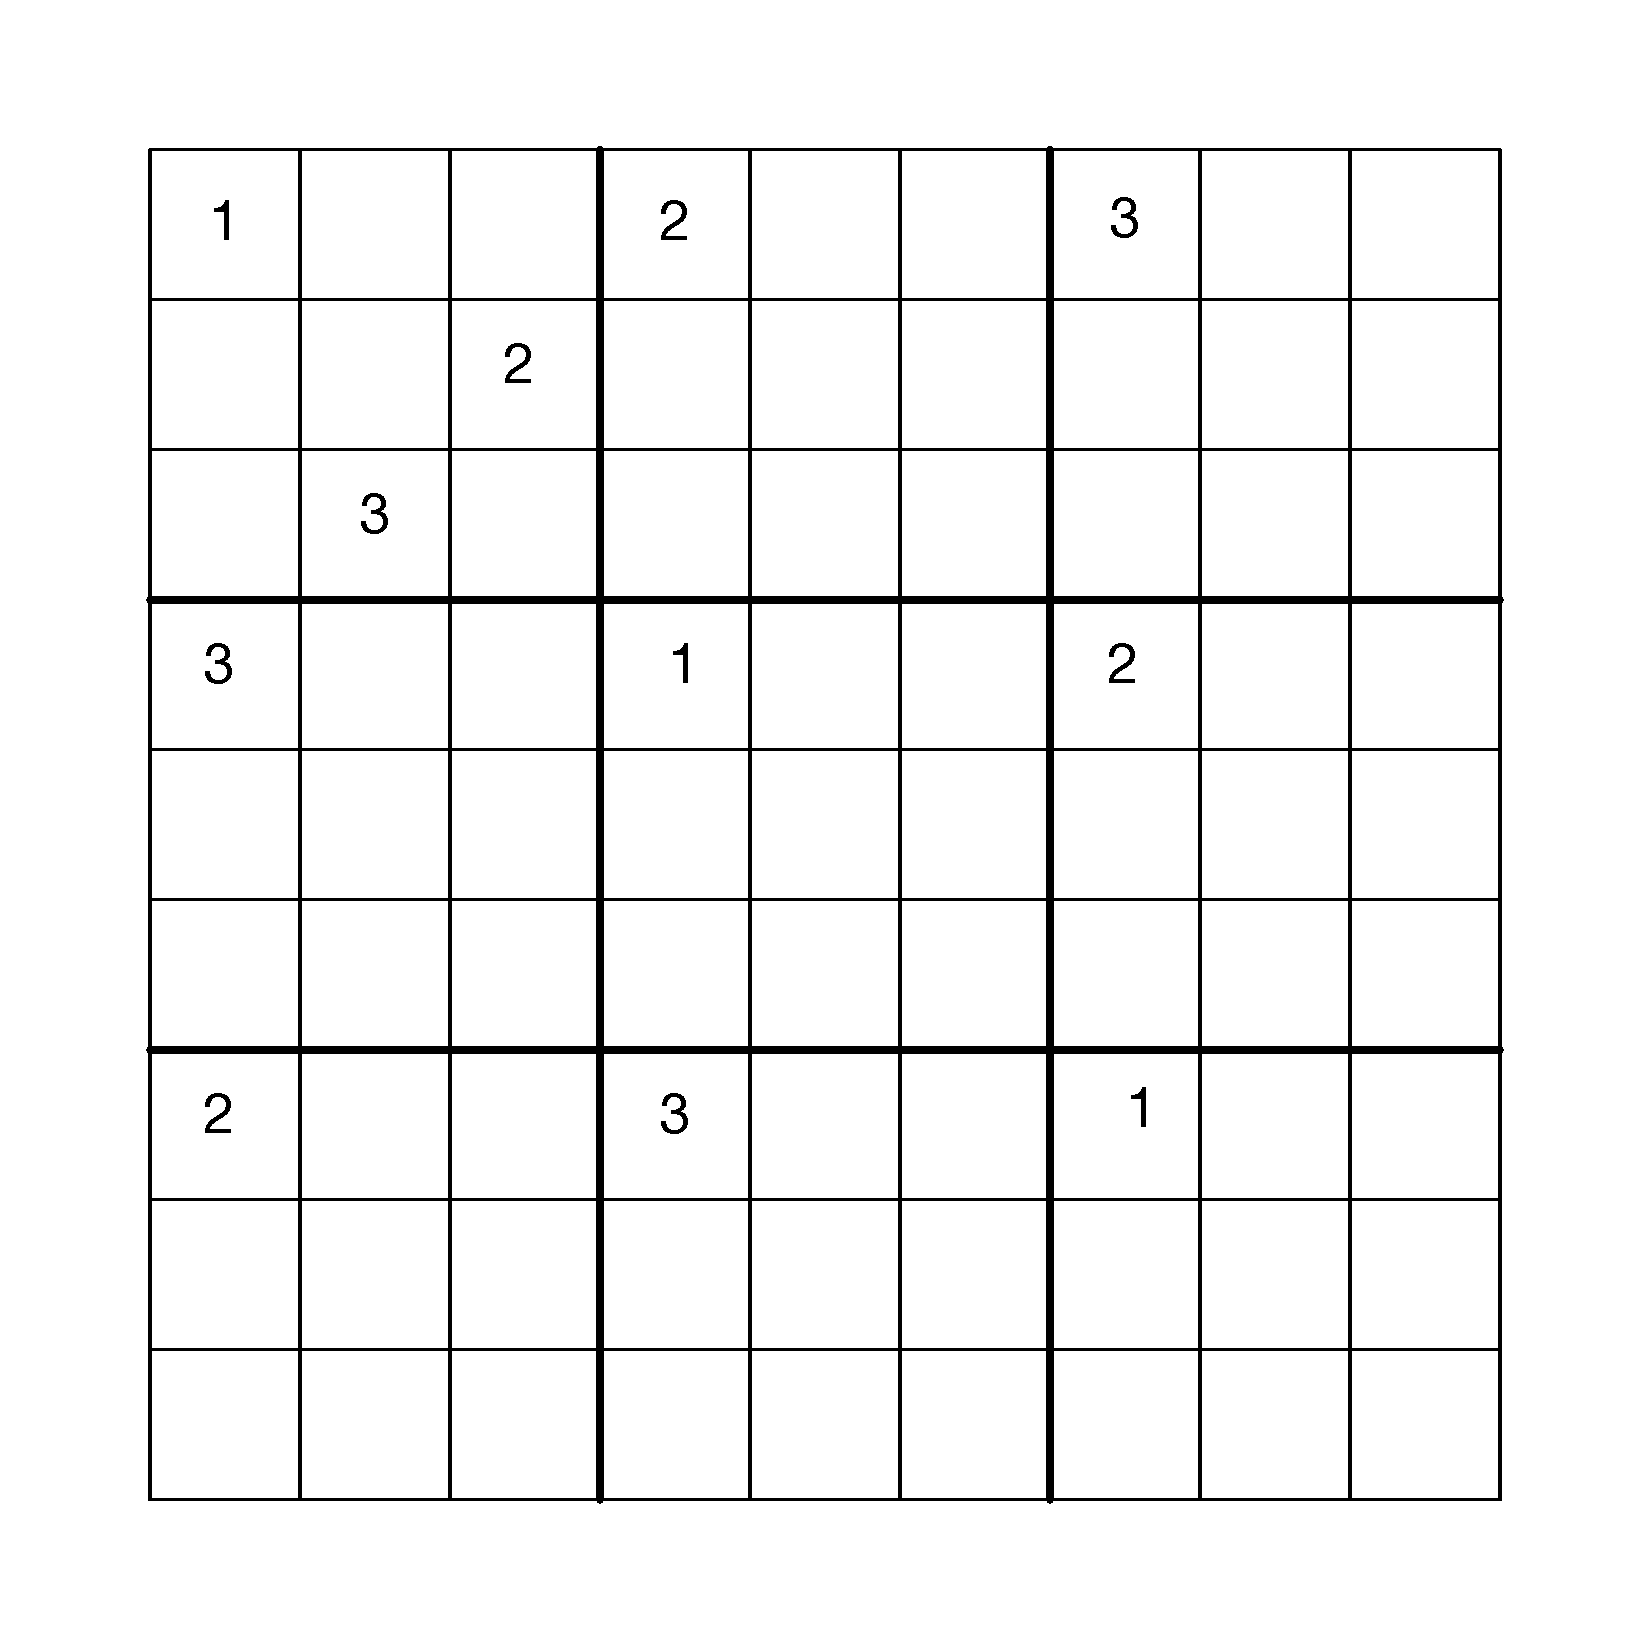
\includegraphics[width=0.45\textwidth]{sudoku}
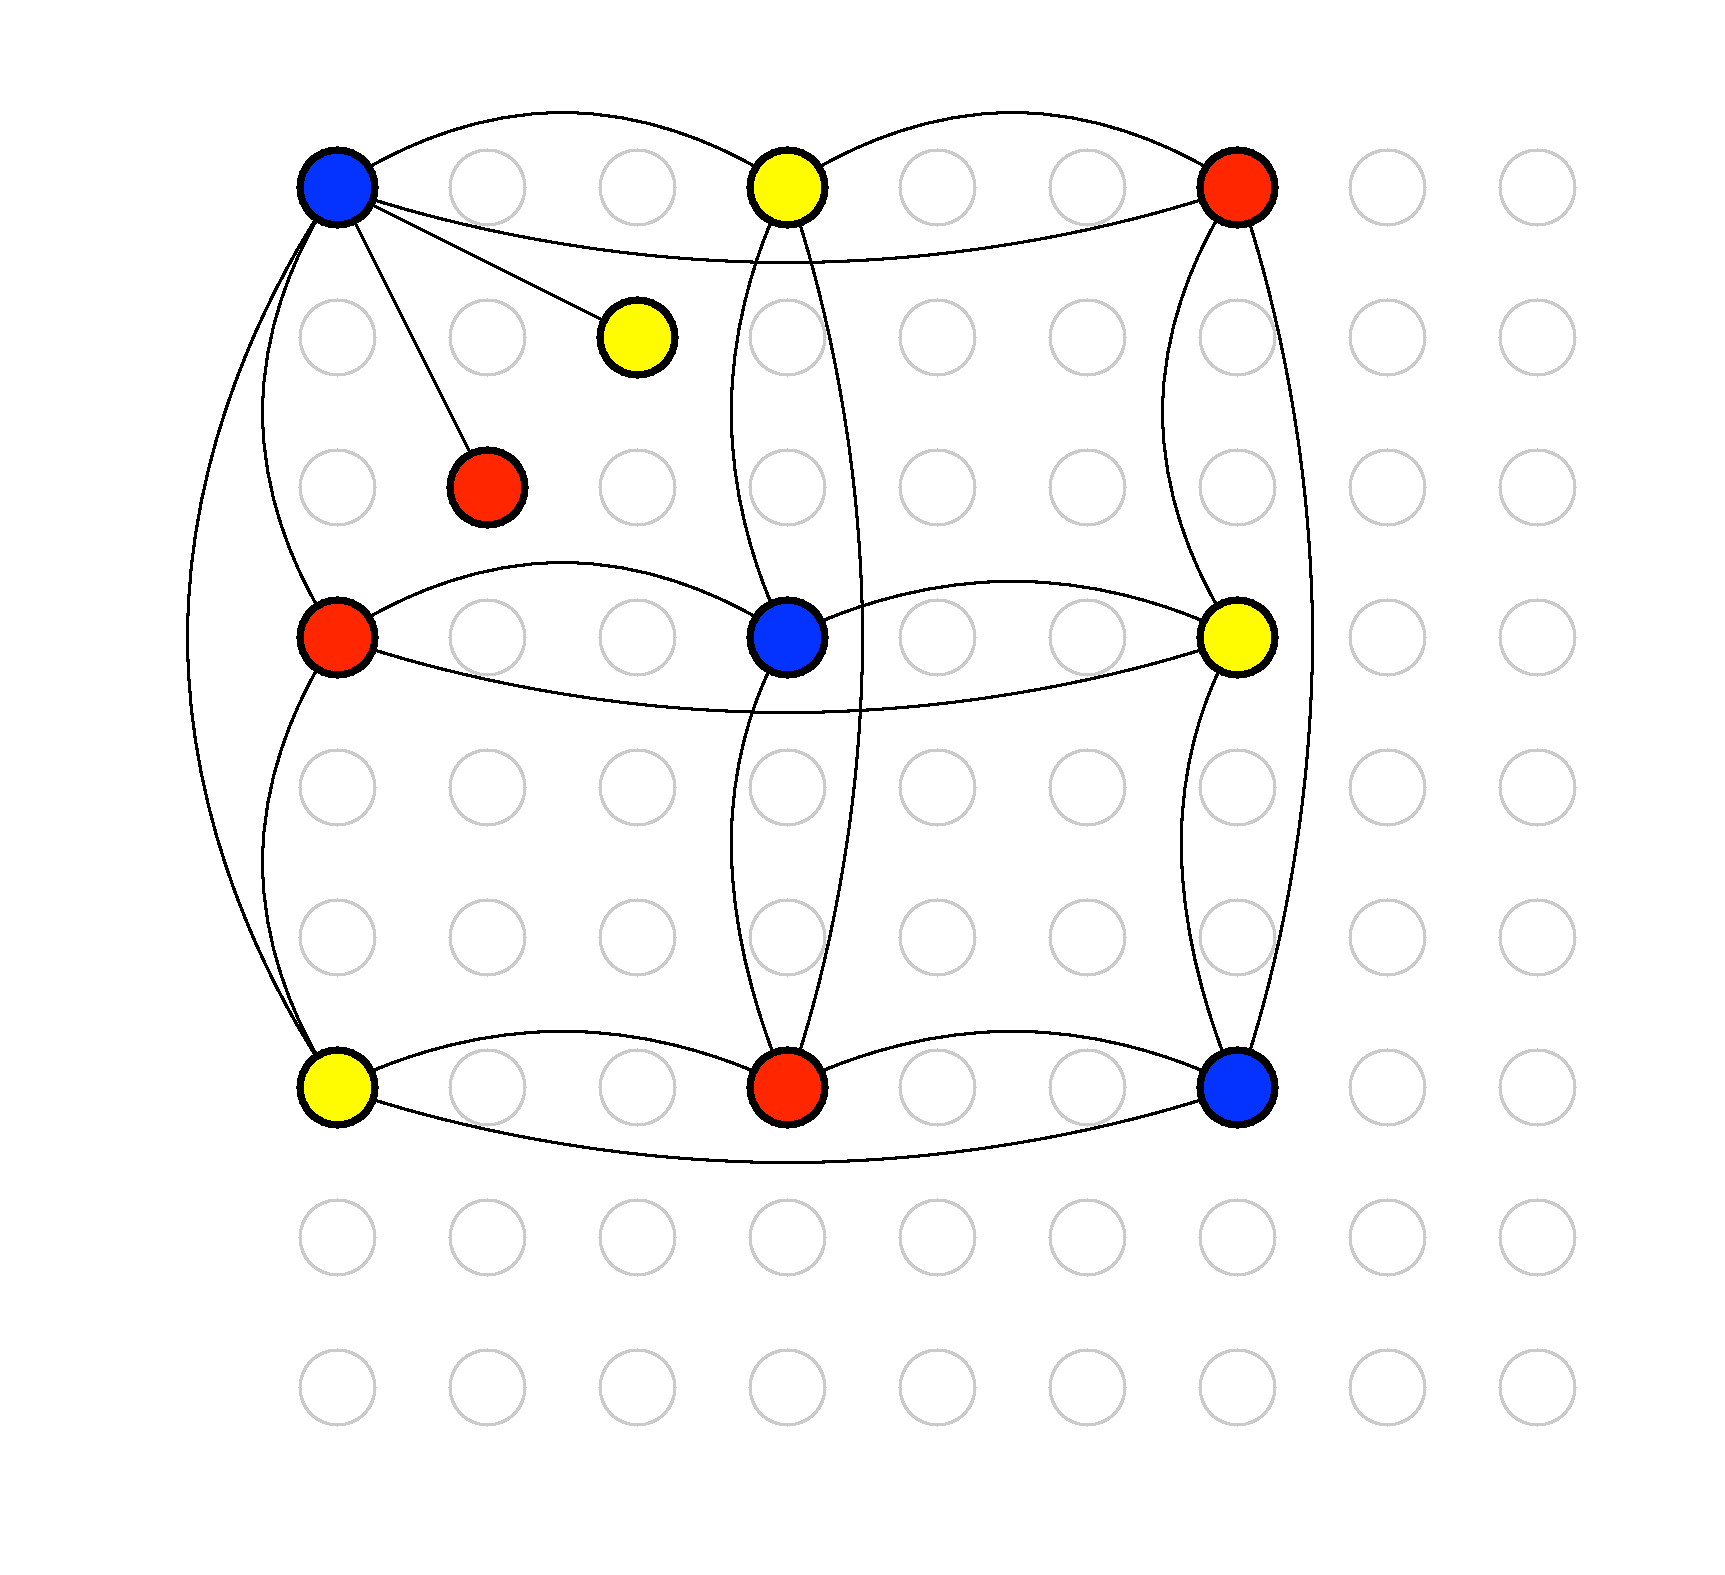
\includegraphics[width=0.5\textwidth]{sudoku-graph}
\caption{A Sudoku game board and the corresponding colored graph.  We
  map the Sudoku number 1 to blue, 2 to yellow, and 3 to red.  We only
  show edges for a sampling of the vertices (those that are colored)
  because showing edges for all of the vertices would make the graph
  unreadable.}
\label{fig:sudoku-graph}
\end{figure}


Given that Sudoku is graph coloring, one can use Sudoku strategies to
come up with an algorithm for allocating registers. For example, one
of the basic techniques for Sudoku is called Pencil Marks. The idea is
that you use a process of elimination to determine what numbers no
longer make sense for a square, and write down those numbers in the
square (writing very small). For example, if the number $1$ is
assigned to a square, then by process of elimination, you can write
the pencil mark $1$ in all the squares in the same row, column, and
region. Many Sudoku computer games provide automatic support for
Pencil Marks. This heuristic also reduces the degree of branching in
the search tree.

The Pencil Marks technique corresponds to the notion of color
\emph{saturation} due to \cite{Brelaz:1979eu}.  The saturation of a
node, in Sudoku terms, is the set of colors that are no longer
available. In graph terminology, we have the following definition:
\begin{equation*}
  \mathrm{saturation}(u) = \{ c \;|\; \exists v. v \in \mathrm{adjacent}(u) 
     \text{ and } \mathrm{color}(v) = c \}
\end{equation*}
where $\mathrm{adjacent}(u)$ is the set of nodes adjacent to $u$.

Using the Pencil Marks technique leads to a simple strategy for
filling in numbers: if there is a square with only one possible number
left, then write down that number! But what if there are no squares
with only one possibility left? One brute-force approach is to just
make a guess. If that guess ultimately leads to a solution, great.  If
not, backtrack to the guess and make a different guess.  Of course,
backtracking can be horribly time consuming. One standard way to
reduce the amount of backtracking is to use the most-constrained-first
heuristic. That is, when making a guess, always choose a square with
the fewest possibilities left (the node with the highest saturation).
The idea is that choosing highly constrained squares earlier rather
than later is better because later there may not be any possibilities.

In some sense, register allocation is easier than Sudoku because we
can always cheat and add more numbers by mapping variables to the
stack. We say that a variable is \emph{spilled} when we decide to map
it to a stack location. We would like to minimize the time needed to
color the graph, and backtracking is expensive. Thus, it makes sense
to keep the most-constrained-first heuristic but drop the backtracking
in favor of greedy search (guess and just keep going).
Figure~\ref{fig:satur-algo} gives the pseudo-code for this simple
greedy algorithm for register allocation based on saturation and the
most-constrained-first heuristic, which is roughly equivalent to the
DSATUR algorithm of \cite{Brelaz:1979eu} (also known as saturation
degree ordering~\citep{Gebremedhin:1999fk,Omari:2006uq}).  Just
as in Sudoku, the algorithm represents colors with integers, with the
first $k$ colors corresponding to the $k$ registers in a given machine
and the rest of the integers corresponding to stack locations.

\begin{figure}[btp]
  \centering
\begin{lstlisting}[basicstyle=\rmfamily,deletekeywords={for,from,with,is,not,in,find},morekeywords={while},columns=fullflexible]
Algorithm: DSATUR
Input: a graph |$G$|
Output: an assignment |$\mathrm{color}[v]$| for each node |$v \in G$|

|$W \gets \mathit{vertices}(G)$|
while |$W \neq \emptyset$| do
    pick a node |$u$| from |$W$| with the highest saturation,
        breaking ties randomly
    find the lowest color |$c$| that is not in |$\{ \mathrm{color}[v] \;:\; v \in \mathrm{adjacent}(v)\}$|
    |$\mathrm{color}[u] \gets c$|
    |$W \gets W - \{u\}$|
\end{lstlisting}
  \caption{Saturation-based greedy graph coloring algorithm.}
  \label{fig:satur-algo}
\end{figure}

With this algorithm in hand, let us return to the running example and
consider how to color the interference graph in
Figure~\ref{fig:interfere}. We shall not use register \key{rax} for
register allocation because we use it to patch instructions, so we
remove that vertex from the graph.  Initially, all of the nodes are
not yet colored and they are unsaturated, so we annotate each of them
with a dash for their color and an empty set for the saturation.
\[
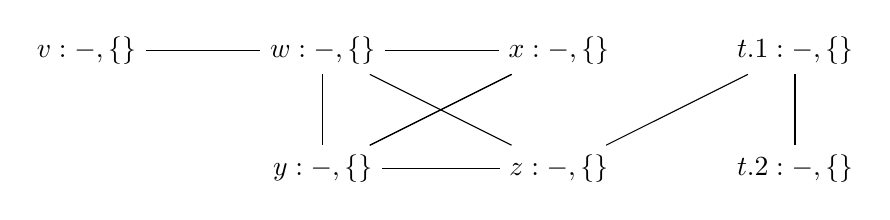
\begin{tikzpicture}[baseline=(current  bounding  box.center)]
\node (v) at (0,0)    {$v:-,\{\}$};
\node (w) at (3,0)    {$w:-,\{\}$};
\node (x) at (6,0)    {$x:-,\{\}$};
\node (y) at (3,-1.5) {$y:-,\{\}$};
\node (z) at (6,-1.5) {$z:-,\{\}$};
\node (t1) at (9,0)   {$t.1:-,\{\}$};
\node (t2) at (9,-1.5) {$t.2:-,\{\}$};

\draw (v) to (w);
\foreach \i in {w,x,y} 
{
  \foreach \j in {w,x,y}
  { 
    \draw (\i) to (\j);
  }
}
\draw (z) to (w);
\draw (z) to (y);
\draw (t1) to (z);
\draw (t2) to (t1);
\end{tikzpicture}
\]
We select a maximally saturated node and color it $0$. In this case we
have a 7-way tie, so we arbitrarily pick $y$. The then mark color $0$
as no longer available for $w$, $x$, and $z$ because they interfere
with $y$.
\[
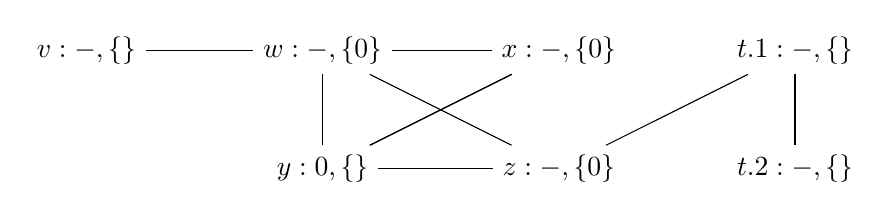
\begin{tikzpicture}[baseline=(current  bounding  box.center)]
\node (v) at (0,0)    {$v:-,\{\}$};
\node (w) at (3,0)    {$w:-,\{0\}$};
\node (x) at (6,0)    {$x:-,\{0\}$};
\node (y) at (3,-1.5) {$y:0,\{\}$};
\node (z) at (6,-1.5) {$z:-,\{0\}$};
\node (t1) at (9,0)   {$t.1:-,\{\}$};
\node (t2) at (9,-1.5) {$t.2:-,\{\}$};
\draw (v) to (w);
\foreach \i in {w,x,y} 
{
  \foreach \j in {w,x,y}
  { 
    \draw (\i) to (\j);
  }
}
\draw (z) to (w);
\draw (z) to (y);
\draw (t1) to (z);
\draw (t2) to (t1);
\end{tikzpicture}
\]
Now we repeat the process, selecting another maximally saturated node.
This time there is a three-way tie between $w$, $x$, and $z$. We color
$w$ with $1$.
\[
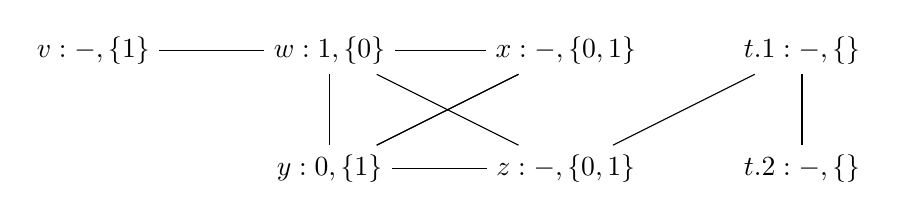
\begin{tikzpicture}[baseline=(current  bounding  box.center)]
\node (v) at (0,0)    {$v:-,\{1\}$};
\node (w) at (3,0)    {$w:1,\{0\}$};
\node (x) at (6,0)    {$x:-,\{0,1\}$};
\node (y) at (3,-1.5) {$y:0,\{1\}$};
\node (z) at (6,-1.5) {$z:-,\{0,1\}$};
\node (t1) at (9,0)   {$t.1:-,\{\}$};
\node (t2) at (9,-1.5) {$t.2:-,\{\}$};
\draw (t1) to (z);
\draw (t2) to (t1);
\draw (v) to (w);
\foreach \i in {w,x,y} 
{
  \foreach \j in {w,x,y}
  { 
    \draw (\i) to (\j);
  }
}
\draw (z) to (w);
\draw (z) to (y);
\end{tikzpicture}
\]
The most saturated nodes are now $x$ and $z$. We color $x$ with the
next available color which is $2$.
\[
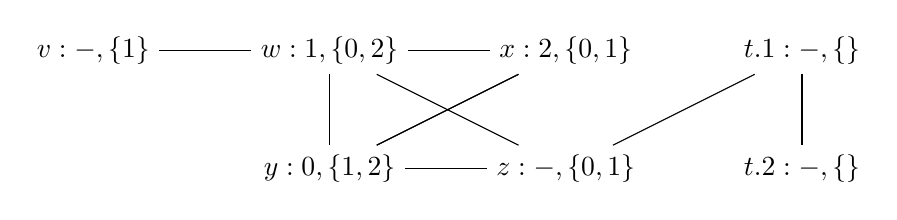
\begin{tikzpicture}[baseline=(current  bounding  box.center)]
\node (v) at (0,0)    {$v:-,\{1\}$};
\node (w) at (3,0)    {$w:1,\{0,2\}$};
\node (x) at (6,0)    {$x:2,\{0,1\}$};
\node (y) at (3,-1.5) {$y:0,\{1,2\}$};
\node (z) at (6,-1.5) {$z:-,\{0,1\}$};
\node (t1) at (9,0)   {$t.1:-,\{\}$};
\node (t2) at (9,-1.5) {$t.2:-,\{\}$};
\draw (t1) to (z);
\draw (t2) to (t1);
\draw (v) to (w);
\foreach \i in {w,x,y} 
{
  \foreach \j in {w,x,y}
  { 
    \draw (\i) to (\j);
  }
}
\draw (z) to (w);
\draw (z) to (y);
\end{tikzpicture}
\]
Node $z$ is the next most highly saturated, so we color $z$ with $2$.
\[
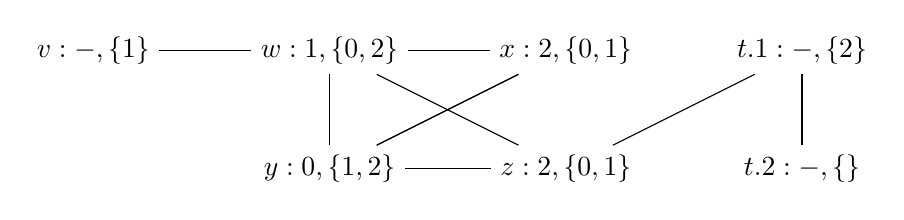
\begin{tikzpicture}[baseline=(current  bounding  box.center)]
\node (v) at (0,0)   {$v:-,\{1\}$};
\node (w) at (3,0)   {$w:1,\{0,2\}$};
\node (x) at (6,0)   {$x:2,\{0,1\}$};
\node (y) at (3,-1.5)  {$y:0,\{1,2\}$};
\node (z) at (6,-1.5)  {$z:2,\{0,1\}$};
\node (t1) at (9,0)   {$t.1:-,\{2\}$};
\node (t2) at (9,-1.5) {$t.2:-,\{\}$};
\draw (t1) to (z);
\draw (t2) to (t1);
\draw (v) to (w);
\foreach \i in {w,x,y} 
{
  \foreach \j in {w,x,y}
  { 
    \draw (\i) to (\j);
  }
}
\draw (z) to (w);
\draw (z) to (y);
\end{tikzpicture}
\]
We have a 2-way tie between $v$ and $t.1$. We choose to color $v$ with
$0$.
\[
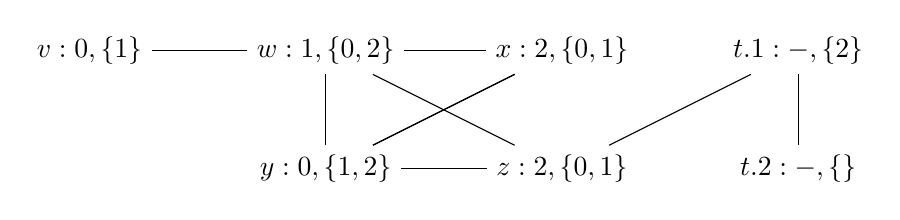
\begin{tikzpicture}[baseline=(current  bounding  box.center)]
\node (v) at (0,0)   {$v:0,\{1\}$};
\node (w) at (3,0)   {$w:1,\{0,2\}$};
\node (x) at (6,0)   {$x:2,\{0,1\}$};
\node (y) at (3,-1.5)  {$y:0,\{1,2\}$};
\node (z) at (6,-1.5)  {$z:2,\{0,1\}$};
\node (t1) at (9,0)   {$t.1:-,\{2\}$};
\node (t2) at (9,-1.5) {$t.2:-,\{\}$};
\draw (t1) to (z);
\draw (t2) to (t1);
\draw (v) to (w);
\foreach \i in {w,x,y} 
{
  \foreach \j in {w,x,y}
  { 
    \draw (\i) to (\j);
  }
}
\draw (z) to (w);
\draw (z) to (y);
\end{tikzpicture}
\]
In the last two steps of the algorithm, we color $t.1$ with $0$
then $t.2$ with $1$.
\[
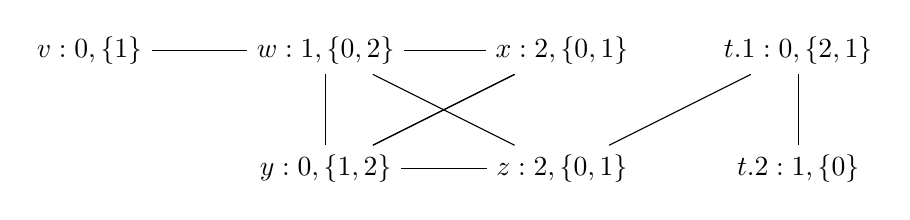
\begin{tikzpicture}[baseline=(current  bounding  box.center)]
\node (v) at (0,0)   {$v:0,\{1\}$};
\node (w) at (3,0)   {$w:1,\{0,2\}$};
\node (x) at (6,0)   {$x:2,\{0,1\}$};
\node (y) at (3,-1.5)  {$y:0,\{1,2\}$};
\node (z) at (6,-1.5)  {$z:2,\{0,1\}$};
\node (t1) at (9,0)   {$t.1:0,\{2,1\}$};
\node (t2) at (9,-1.5) {$t.2:1,\{0\}$};
\draw (t1) to (z);
\draw (t2) to (t1);
\draw (v) to (w);
\foreach \i in {w,x,y} 
{
  \foreach \j in {w,x,y}
  { 
    \draw (\i) to (\j);
  }
}
\draw (z) to (w);
\draw (z) to (y);
\end{tikzpicture}
\]


With the coloring complete, we can finalize the assignment of
variables to registers and stack locations. Recall that if we have $k$
registers, we map the first $k$ colors to registers and the rest to
stack locations.  Suppose for the moment that we just have one extra
register to use for register allocation, just \key{rbx}. Then the
following is the mapping of colors to registers and stack allocations.
\[
  \{ 0 \mapsto \key{\%rbx}, \; 1 \mapsto \key{-8(\%rbp)}, \; 2 \mapsto \key{-16(\%rbp)}, \ldots \}
\]
Putting this mapping together with the above coloring of the variables, we
arrive at the assignment:
\begin{gather*}
  \{ v \mapsto \key{\%rbx}, \,
  w \mapsto \key{-8(\%rbp)},  \,
  x \mapsto \key{-16(\%rbp)}, \,
  y \mapsto \key{\%rbx},  \,
  z\mapsto \key{-16(\%rbp)}, \\
  t.1\mapsto \key{\%rbx} ,\,
  t.2\mapsto \key{-8(\%rbp)} \}
\end{gather*}
Applying this assignment to our running example
(Figure~\ref{fig:reg-eg}) yields the program on the right.

% why frame size of 32? -JGS
\begin{minipage}{0.45\textwidth}
\begin{lstlisting}
  (program (v w x y z)
    (movq (int 1) (var v))
    (movq (int 46) (var w))
    (movq (var v) (var x))
    (addq (int 7) (var x))
    (movq (var x) (var y))
    (addq (int 4) (var y))
    (movq (var x) (var z))
    (addq (var w) (var z))
    (movq (var y) (var t.1))
    (negq (var t.1))
    (movq (var z) (var t.2))
    (addq (var t.1) (var t.2))
    (movq (var t.2) (reg rax)))
\end{lstlisting}
\end{minipage}
$\Rightarrow$
\begin{minipage}{0.45\textwidth}
\begin{lstlisting}
(program 16
  (movq (int 1) (reg rbx))
  (movq (int 46) (stack -8))
  (movq (reg rbx) (stack -16))
  (addq (int 7) (stack -16))
  (movq (stack 16) (reg rbx))
  (addq (int 4) (reg rbx))
  (movq (stack -16) (stack -16))
  (addq (stack -8) (stack -16))
  (movq (reg rbx) (reg rbx))
  (negq (reg rbx))
  (movq (stack -16) (stack -8))
  (addq (reg rbx) (stack -8))
  (movq (stack -8) (reg rax)))
\end{lstlisting}
\end{minipage}

The resulting program is almost an x86 program. The remaining step
is to apply the patch instructions pass. In this example, the trivial
move of \code{-16(\%rbp)} to itself is deleted and the addition of
\code{-8(\%rbp)} to \key{-16(\%rbp)} is fixed by going through
\code{rax}. The following shows the portion of the program that
changed.
\begin{lstlisting}
  (addq (int 4) (reg rbx))
  (movq (stack -8) (reg rax)
  (addq (reg rax) (stack -16))
\end{lstlisting}
An overview of all of the passes involved in register allocation is
shown in Figure~\ref{fig:reg-alloc-passes}.

\begin{figure}[p]
\begin{tikzpicture}[baseline=(current  bounding  box.center)]
\node (R1) at (0,2)  {\large $R_1$};
\node (R1-2) at (3,2)  {\large $R_1$};
\node (C0-1) at (3,0)  {\large $C_0$};

\node (x86-2) at (3,-2)  {\large $\text{x86}^{*}$};
\node (x86-3) at (6,-2)  {\large $\text{x86}^{*}$};
\node (x86-4) at (9,-2) {\large $\text{x86}$};
\node (x86-5) at (12,-2) {\large $\text{x86}^{\dagger}$};

\node (x86-2-1) at (3,-4)  {\large $\text{x86}^{*}$};
\node (x86-2-2) at (6,-4)  {\large $\text{x86}^{*}$};

\path[->,bend left=15] (R1) edge [above] node {\ttfamily\footnotesize uniquify} (R1-2);
\path[->,bend left=15] (R1-2) edge [right] node {\ttfamily\footnotesize flatten} (C0-1);
\path[->,bend right=15] (C0-1) edge [left] node {\ttfamily\footnotesize select-instr.} (x86-2);
\path[->,bend left=15] (x86-2) edge [right] node {\ttfamily\footnotesize uncover-live} (x86-2-1);
\path[->,bend right=15] (x86-2-1) edge [below] node {\ttfamily\footnotesize build-inter.} (x86-2-2);
\path[->,bend right=15] (x86-2-2) edge [right] node {\ttfamily\footnotesize allocate-reg.} (x86-3);
\path[->,bend left=15] (x86-3) edge [above] node {\ttfamily\footnotesize patch-instr.} (x86-4);
\path[->,bend left=15] (x86-4) edge [above] node {\ttfamily\footnotesize print-x86} (x86-5);
\end{tikzpicture}
\caption{Diagram of the passes for compiling $R_1$, including the
  three new passes for register allocation.}
\label{fig:reg-alloc-passes}
\end{figure}

\begin{exercise}\normalfont
Implement the pass \code{allocate-registers} and test it by creating
new example programs that exercise all of the register allocation
algorithm, such as forcing variables to be spilled to the stack.

I recommend organizing our code by creating a helper function named
\code{allocate-homes} that takes an interference graph, a list of all
the variables in the program, and the list of statements. This
function should return a mapping of variables to their homes
(registers or stack locations) and the total size needed for the
stack. By creating this helper function, we will be able to reuse it
in Chapter~\ref{ch:functions} when we add support for functions.

Once you have obtained the mapping from \code{allocate-homes}, you can
use the \code{assign-homes} function from Section~\ref{sec:assign-s0}
to replace the variables with their homes.
\end{exercise}


\section{Print x86 and Conventions for Registers}
\label{sec:print-x86-reg-alloc}

Recall the the \code{print-x86} pass generates the prelude and
conclusion instructions for the \code{main} function.  The prelude
saved the values in \code{rbp} and \code{rsp} and the conclusion
returned those values to \code{rbp} and \code{rsp}. The reason for
this is that there are agreed-upon conventions for how different
functions share the same fixed set of registers. There is a function
inside the operating system (OS) that calls our \code{main} function,
and that OS function uses the same registers that we use in
\code{main}. The convention for x86 is that the caller is responsible
for freeing up some registers, the \emph{caller save registers}, prior
to the function call, and the callee is responsible for saving and
restoring some other registers, the \emph{callee save registers},
before and after using them. The caller save registers are
\begin{lstlisting}
  rax rdx rcx rsi rdi r8 r9 r10 r11
\end{lstlisting}
while the callee save registers are 
\begin{lstlisting}
  rsp rbp rbx r12 r13 r14 r15
\end{lstlisting}
Another way to think about this caller/callee convention is the
following. The caller should assume that all the caller save registers
get overwritten with arbitrary values by the callee.  On the other
hand, the caller can safely assume that all the callee save registers
contain the same values after the call that they did before the call.
The callee can freely use any of the caller save registers.  However,
if the callee wants to use a callee save register, the callee must
arrange to put the original value back in the register prior to
returning to the caller, which is usually accomplished by saving and
restoring the value from the stack.

The upshot of these conventions is that the \code{main} function needs
to save (in the prelude) and restore (in the conclusion) any callee
save registers that get used during register allocation. The simplest
approach is to save and restore all the callee save registers. The
more efficient approach is to keep track of which callee save
registers were used and only save and restore them. Either way, make
sure to take this use of stack space into account when you round up
the size of the frame to make sure it is a multiple of 16 bytes.

\section{Challenge: Move Biasing$^{*}$}
\label{sec:move-biasing}

This section describes an optional enhancement to register allocation
for those students who are looking for an extra challenge or who have
a deeper interest in register allocation.

We return to the running example, but we remove the supposition that
we only have one register to use. So we have the following mapping of
color numbers to registers.
\[
  \{ 0 \mapsto \key{\%rbx}, \; 1 \mapsto \key{\%rcx}, \; 2 \mapsto \key{\%rdx}, \ldots \}
\]
Using the same assignment that was produced by register allocator
described in the last section, we get the following program.

\begin{minipage}{0.45\textwidth}
\begin{lstlisting}
  (program (v w x y z)
    (movq (int 1) (var v))
    (movq (int 46) (var w))
    (movq (var v) (var x))
    (addq (int 7) (var x))
    (movq (var x) (var y))
    (addq (int 4) (var y))
    (movq (var x) (var z))
    (addq (var w) (var z))
    (movq (var y) (var t.1))
    (negq (var t.1))
    (movq (var z) (var t.2))
    (addq (var t.1) (var t.2))
    (movq (var t.2) (reg rax)))
\end{lstlisting}
\end{minipage}
$\Rightarrow$
\begin{minipage}{0.45\textwidth}
\begin{lstlisting}
(program 0
  (movq (int 1) (reg rbx))
  (movq (int 46) (reg rcx))
  (movq (reg rbx) (reg rdx))
  (addq (int 7) (reg rdx))
  (movq (reg rdx) (reg rbx))
  (addq (int 4) (reg rbx))
  (movq (reg rdx) (reg rdx))
  (addq (reg rcx) (reg rdx))
  (movq (reg rbx) (reg rbx))
  (negq (reg rbx))
  (movq (reg rdx) (reg rcx))
  (addq (reg rbx) (reg rcx))
  (movq (reg rcx) (reg rax)))
\end{lstlisting}
\end{minipage}

While this allocation is quite good, we could do better. For example,
the variables \key{v} and \key{x} ended up in different registers, but
if they had been placed in the same register, then the move from
\key{v} to \key{x} could be removed. 

We say that two variables $p$ and $q$ are \emph{move related} if they
participate together in a \key{movq} instruction, that is, \key{movq
  p, q} or \key{movq q, p}. When the register allocator chooses a
color for a variable, it should prefer a color that has already been
used for a move-related variable (assuming that they do not
interfere). Of course, this preference should not override the
preference for registers over stack locations, but should only be used
as a tie breaker when choosing between registers or when choosing
between stack locations.

We recommend that you represent the move relationships in a graph,
similar to how we represented interference.  The following is the
\emph{move graph} for our running example.
\[
\begin{tikzpicture}[baseline=(current  bounding  box.center)]
\node (v) at (0,0)    {$v$};
\node (w) at (3,0)    {$w$};
\node (x) at (6,0)    {$x$};
\node (y) at (3,-1.5) {$y$};
\node (z) at (6,-1.5) {$z$};
\node (t1) at (9,0)   {$t.1$};
\node (t2) at (9,-1.5) {$t.2$};
\draw (t1) to (y);
\draw (t2) to (z);
\draw[bend left=20] (v) to (x);
\draw (x) to (y);
\draw (x) to (z);
\end{tikzpicture}
\]

Now we replay the graph coloring, pausing to see the coloring of $z$
and $v$. So we have the following coloring so far and the most
saturated vertex is $z$.
\[
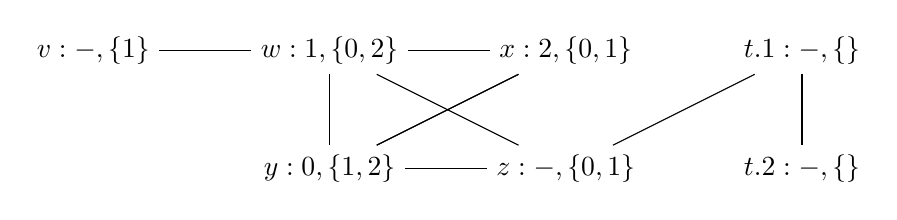
\begin{tikzpicture}[baseline=(current  bounding  box.center)]
\node (v) at (0,0)    {$v:-,\{1\}$};
\node (w) at (3,0)    {$w:1,\{0,2\}$};
\node (x) at (6,0)    {$x:2,\{0,1\}$};
\node (y) at (3,-1.5) {$y:0,\{1,2\}$};
\node (z) at (6,-1.5) {$z:-,\{0,1\}$};
\node (t1) at (9,0)   {$t.1:-,\{\}$};
\node (t2) at (9,-1.5) {$t.2:-,\{\}$};
\draw (t1) to (z);
\draw (t2) to (t1);
\draw (v) to (w);
\foreach \i in {w,x,y} 
{
  \foreach \j in {w,x,y}
  { 
    \draw (\i) to (\j);
  }
}
\draw (z) to (w);
\draw (z) to (y);
\end{tikzpicture}
\]
Last time we chose to color $z$ with $2$, which so happens to be the
color of $x$, and $z$ is move related to $x$. This was rather lucky,
and if the program had been a little different, and say $x$ had been
already assigned to $3$, then $z$ would still get $2$ and our luck
would have run out. With move biasing, we use the fact that $z$ and
$x$ are move related to influence the choice of color for $z$, in this
case choosing $2$ because that's the color of $x$.
\[
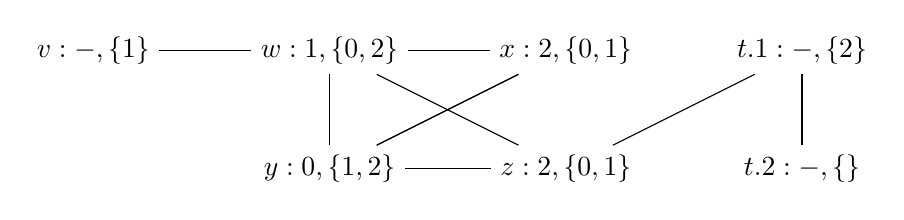
\begin{tikzpicture}[baseline=(current  bounding  box.center)]
\node (v) at (0,0)    {$v:-,\{1\}$};
\node (w) at (3,0)    {$w:1,\{0,2\}$};
\node (x) at (6,0)    {$x:2,\{0,1\}$};
\node (y) at (3,-1.5) {$y:0,\{1,2\}$};
\node (z) at (6,-1.5) {$z:2,\{0,1\}$};
\node (t1) at (9,0)   {$t.1:-,\{2\}$};
\node (t2) at (9,-1.5) {$t.2:-,\{\}$};
\draw (t1) to (z);
\draw (t2) to (t1);
\draw (v) to (w);
\foreach \i in {w,x,y} 
{
  \foreach \j in {w,x,y}
  { 
    \draw (\i) to (\j);
  }
}
\draw (z) to (w);
\draw (z) to (y);
\end{tikzpicture}
\]

Next we consider coloring the variable $v$, and we just need to avoid
choosing $1$ because of the interference with $w$. Last time we choose
the color $0$, simply because it was the lowest, but this time we know
that $v$ is move related to $x$, so we choose the color $2$.
\[
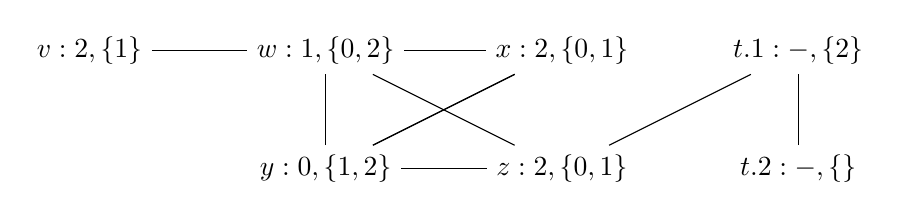
\begin{tikzpicture}[baseline=(current  bounding  box.center)]
\node (v) at (0,0)    {$v:2,\{1\}$};
\node (w) at (3,0)    {$w:1,\{0,2\}$};
\node (x) at (6,0)    {$x:2,\{0,1\}$};
\node (y) at (3,-1.5) {$y:0,\{1,2\}$};
\node (z) at (6,-1.5) {$z:2,\{0,1\}$};
\node (t1) at (9,0)   {$t.1:-,\{2\}$};
\node (t2) at (9,-1.5) {$t.2:-,\{\}$};
\draw (t1) to (z);
\draw (t2) to (t1);
\draw (v) to (w);
\foreach \i in {w,x,y} 
{
  \foreach \j in {w,x,y}
  { 
    \draw (\i) to (\j);
  }
}
\draw (z) to (w);
\draw (z) to (y);
\end{tikzpicture}
\]

We apply this register assignment to the running example, on the left,
to obtain the code on right.

\begin{minipage}{0.45\textwidth}
\begin{lstlisting}
  (program (v w x y z)
    (movq (int 1) (var v))
    (movq (int 46) (var w))
    (movq (var v) (var x))
    (addq (int 7) (var x))
    (movq (var x) (var y))
    (addq (int 4) (var y))
    (movq (var x) (var z))
    (addq (var w) (var z))
    (movq (var y) (var t.1))
    (negq (var t.1))
    (movq (var z) (var t.2))
    (addq (var t.1) (var t.2))
    (movq (var t.2) (reg rax)))
\end{lstlisting}
\end{minipage}
$\Rightarrow$
\begin{minipage}{0.45\textwidth}
\begin{lstlisting}
(program 0
  (movq (int 1) (reg rdx))
  (movq (int 46) (reg rcx))
  (movq (reg rdx) (reg rdx))
  (addq (int 7) (reg rdx))
  (movq (reg rdx) (reg rbx))
  (addq (int 4) (reg rbx))
  (movq (reg rdx) (reg rdx))
  (addq (reg rcx) (reg rdx))
  (movq (reg rbx) (reg rbx))
  (negq (reg rbx))
  (movq (reg rdx) (reg rcx))
  (addq (reg rbx) (reg rcx))
  (movq (reg rcx) (reg rax)))
\end{lstlisting}
\end{minipage}

The \code{patch-instructions} then removes the trivial moves from
\key{v} to \key{x}, from \key{x} to \key{z}, and from \key{y} to
\key{t.1}, to obtain the following result.
\begin{lstlisting}
(program 0
  (movq (int 1) (reg rdx))
  (movq (int 46) (reg rcx))
  (addq (int 7) (reg rdx))
  (movq (reg rdx) (reg rbx))
  (addq (int 4) (reg rbx))
  (addq (reg rcx) (reg rdx))
  (negq (reg rbx))
  (movq (reg rdx) (reg rcx))
  (addq (reg rbx) (reg rcx))
  (movq (reg rcx) (reg rax)))
\end{lstlisting}

\begin{exercise}\normalfont
Change your implementation of \code{allocate-registers} to take move
biasing into account. Make sure that your compiler still passes all of
the previous tests. Create two new tests that include at least one
opportunity for move biasing and visually inspect the output x86
programs to make sure that your move biasing is working properly.
\end{exercise}



%%%%%%%%%%%%%%%%%%%%%%%%%%%%%%%%%%%%%%%%%%%%%%%%%%%%%%%%%%%%%%%%%%%%%%%%%%%%%%%%
\chapter{Booleans, Control Flow, and Type Checking}
\label{ch:bool-types}

Up until now the input languages have only included a single kind of
value, the integers. In this Chapter we add a second kind of value,
the Booleans (true and false), together with some new operations
(\key{and}, \key{not}, \key{eq?}) and conditional expressions to create
the $R_2$ language.  With the addition of conditional expressions,
programs can have non-trivial control flow which has an impact on
several parts of the compiler. Also, because we now have two kinds of
values, we need to worry about programs that apply an operation to the
wrong kind of value, such as \code{(not 1)}.

There are two language design options for such situations.  One option
is to signal an error and the other is to provide a wider
interpretation of the operation. The Racket language uses a mixture of
these two options, depending on the operation and on the kind of
value. For example, the result of \code{(not 1)} in Racket is
\code{\#f} (that is, false) because Racket treats non-zero integers as
true. On the other hand, \code{(car 1)} results in a run-time error in
Racket, which states that \code{car} expects a pair.

The Typed Racket language makes similar design choices as Racket,
except much of the error detection happens at compile time instead of
run time. Like Racket, Typed Racket accepts and runs \code{(not 1)},
producing \code{\#f}. But in the case of \code{(car 1)}, Typed Racket
reports a compile-time error because the type of the argument is
expected to be of the form \code{(Listof T)} or \code{(Pairof T1 T2)}.

For the $R_2$ language we choose to be more like Typed Racket in that
we shall perform type checking during compilation.  However, we shall
take a narrower interpretation of the operations, rejecting
\code{(not 1)}. Despite this difference in design,
$R_2$ is literally a subset of Typed Racket.  Every $R_2$
program is a Typed Racket program.

This chapter is organized as follows.  We begin by defining the syntax
and interpreter for the $R_2$ language (Section~\ref{sec:r2-lang}). We
then introduce the idea of type checking and build a type checker for
$R_2$ (Section~\ref{sec:type-check-r2}). To compile $R_2$ we need to
enlarge the intermediate language $C_0$ into $C_1$, which we do in
Section~\ref{sec:c1}. The remaining sections of this Chapter discuss
how our compiler passes need to change to accommodate Booleans and
conditional control flow.


\section{The $R_2$ Language}
\label{sec:r2-lang}

The syntax of the $R_2$ language is defined in
Figure~\ref{fig:r2-syntax}. It includes all of $R_1$, so we only show
the new operators and expressions. We add the Boolean literals
\code{\#t} and \code{\#f} for true and false and the conditional
expression. The operators are expanded to include the \key{and} and
\key{not} operations on Booleans and the \key{eq?} operation for
comparing two integers and for comparing two Booleans.

\begin{figure}[tbp]
\centering
\fbox{
\begin{minipage}{0.96\textwidth}
\[
\begin{array}{lcl}
  \Exp &::=& \gray{\Int \mid (\key{read}) \mid (\key{-}\;\Exp) \mid (\key{+} \; \Exp\;\Exp)}  \\
     &\mid&  \gray{\Var \mid \LET{\Var}{\Exp}{\Exp}} \mid \key{\#t} \mid \key{\#f} \mid
      (\key{and}\;\Exp\;\Exp) \mid (\key{not}\;\Exp) \\
      &\mid& (\key{eq?}\;\Exp\;\Exp) \mid \IF{\Exp}{\Exp}{\Exp} \\
  R_2 &::=& (\key{program} \; \Exp)
\end{array}
\]
\end{minipage}
}
\caption{The $R_2$ language, an extension of $R_1$
  (Figure~\ref{fig:r1-syntax}).}
\label{fig:r2-syntax}
\end{figure}

Figure~\ref{fig:interp-R2} defines the interpreter for $R_2$, omitting
the parts that are the same as the interpreter for $R_1$
(Figure~\ref{fig:interp-R1}). The literals \code{\#t} and \code{\#f}
simply evaluate to themselves. The conditional expression \code{(if
  cnd thn els)} evaluates the Boolean expression \code{cnd} and then
either evaluates \code{thn} or \code{els} depending on whether
\code{cnd} produced \code{\#t} or \code{\#f}. The logical operations
\code{not} and \code{and} behave as you might expect, but note that
the \code{and} operation is short-circuiting. That is, the second
expression \code{e2} is not evaluated if \code{e1} evaluates to
\code{\#f}.

\begin{figure}[tbp]
\begin{lstlisting}
   (define (interp-R2 env e)
     (match e
       ...
       [(? boolean?) e]
       [`(if ,cnd ,thn ,els)
        (match (interp-R2 env cnd)
          [#t (interp-R2 env thn)]
          [#f (interp-R2 env els)])]
       [`(not ,e)
        (match (interp-R2 env e) [#t #f] [#f #t])]
       [`(and ,e1 ,e2)
         (match (interp-R2 env e1)
           [#t (match (interp-R2 env e2) [#t #t] [#f #f])]
           [#f #f])]
       [`(eq? ,e1 ,e2)
         (let ([v1 (interp-R2 env e1)] [v2 (interp-R2 env e2)])
           (cond [(and (fixnum? v1) (fixnum? v2)) (eq? v1 v2)]
                 [(and (boolean? v1) (boolean? v2)) (eq? v1 v2)]))]
       ))
\end{lstlisting}
\caption{Interpreter for the $R_2$ language.}
\label{fig:interp-R2}
\end{figure}


\section{Type Checking $R_2$ Programs}
\label{sec:type-check-r2}

It is helpful to think about type checking into two complementary
ways. A type checker predicts the \emph{type} of value that will be
produced by each expression in the program.  For $R_2$, we have just
two types, \key{Integer} and \key{Boolean}. So a type checker should
predict that
\begin{lstlisting}
   (+ 10 (- (+ 12 20)))
\end{lstlisting}
produces an \key{Integer} while
\begin{lstlisting}
   (and (not #f) #t)
\end{lstlisting}
produces a \key{Boolean}.

As mentioned at the beginning of this chapter, a type checker also
rejects programs that apply operators to the wrong type of value. Our
type checker for $R_2$ will signal an error for the following because,
as we have seen above, the expression \code{(+ 10 ...)} has type
\key{Integer}, and we shall require an argument of \code{not} to have
type \key{Boolean}.
\begin{lstlisting}
   (not (+ 10 (- (+ 12 20))))
\end{lstlisting}

The type checker for $R_2$ is best implemented as a structurally
recursive function over the AST. Figure~\ref{fig:type-check-R2} shows
many of the clauses for the \code{typecheck-R2} function.  Given an
input expression \code{e}, the type checker either returns the type
(\key{Integer} or \key{Boolean}) or it signals an error.  Of course,
the type of an integer literal is \code{Integer} and the type of a
Boolean literal is \code{Boolean}.  To handle variables, the type
checker, like the interpreter, uses an association list. However, in
this case the association list maps variables to types instead of
values. Consider the clause for \key{let}.  We type check the
initializing expression to obtain its type \key{T} and then map the
variable \code{x} to \code{T}. When the type checker encounters the
use of a variable, it can lookup its type in the association list.

\begin{figure}[tbp]
\begin{lstlisting}
   (define (typecheck-R2 env e)
     (match e
       [(? fixnum?) 'Integer]
       [(? boolean?) 'Boolean]
       [(? symbol?) (lookup e env)]
       [`(let ([,x ,e]) ,body)
        (define T (typecheck-R2 env e))
        (define new-env (cons (cons x T) env))
        (typecheck-R2 new-env body)]
       ...
       [`(not ,e)
        (match (typecheck-R2 env e)
          ['Boolean 'Boolean]
          [else (error 'typecheck-R2 "'not' expects a Boolean" e)])]
       ...
       [`(program ,body)
         (typecheck-R2 '() body)
         `(program ,body)]
       ))
\end{lstlisting}
\caption{Skeleton of a type checker for the $R_2$ language.}
\label{fig:type-check-R2}
\end{figure}

\begin{exercise}\normalfont
Complete the implementation of \code{typecheck-R2} and test it on 10
new example programs in $R_2$ that you choose based on how thoroughly
they test the type checking algorithm. Half of the example programs
should have a type error, to make sure that your type checker properly
rejects them. The other half of the example programs should not have
type errors. Your testing should check that the result of the type
checker agrees with the value returned by the interpreter, that is, if
the type checker returns \key{Integer}, then the interpreter should
return an integer. Likewise, if the type checker returns
\key{Boolean}, then the interpreter should return \code{\#t} or
\code{\#f}. Note that if your type checker does not signal an error
for a program, then interpreting that program should not encounter an
error.  If it does, there is something wrong with your type checker.
\end{exercise}

\section{The $C_1$ Language}
\label{sec:c1}

The $R_2$ language adds Booleans and conditional expressions to $R_1$.
As with $R_1$, we shall compile to a C-like intermediate language, but
we need to grow that intermediate language to handle the new features
in $R_2$. Figure~\ref{fig:c1-syntax} shows the new features of $C_1$;
we add logic and comparison operators to the $\Exp$ non-terminal, the
literals \key{\#t} and \key{\#f} to the $\Arg$ non-terminal, and we
add an \key{if} statement. The \key{if} statement of $C_1$ includes an
\key{eq?} test, which is needed for improving code generation in
Section~\ref{sec:opt-if}.  We do not include \key{and} in $C_1$
because it is not needed in the translation of the \key{and} of $R_2$.

\begin{figure}[tbp]
\fbox{
\begin{minipage}{0.96\textwidth}
\[
\begin{array}{lcl}
\Arg &::=& \gray{\Int \mid \Var} \mid \key{\#t} \mid \key{\#f} \\
\Exp &::= & \gray{\Arg \mid (\key{read}) \mid (\key{-}\;\Arg) \mid (\key{+} \; \Arg\;\Arg)}
      \mid (\key{not}\;\Arg) \mid (\key{eq?}\;\Arg\;\Arg) \\
\Stmt &::=& \gray{\ASSIGN{\Var}{\Exp} \mid \RETURN{\Arg}} \\
      &\mid& \IF{(\key{eq?}\, \Arg\,\Arg)}{\Stmt^{*}}{\Stmt^{*}} \\
C_1 & ::= & (\key{program}\;(\Var^{*})\;\Stmt^{+})
\end{array}
\]
\end{minipage}
}
\caption{The $C_1$ intermediate language, an extension of $C_0$
  (Figure~\ref{fig:c0-syntax}).}
\label{fig:c1-syntax}
\end{figure}

\section{Flatten Expressions}
\label{sec:flatten-r2}

The \code{flatten} pass needs to be expanded to handle the Boolean
literals \key{\#t} and \key{\#f}, the new logic and comparison
operations, and \key{if} expressions. We shall start with a simple
example of translating a \key{if} expression, shown below on the
left. \\
\begin{tabular}{lll}
\begin{minipage}{0.4\textwidth}
\begin{lstlisting}
 (program (if #f 0 42))
\end{lstlisting}
\end{minipage}
&
$\Rightarrow$
&
\begin{minipage}{0.4\textwidth}
\begin{lstlisting}
(program (if.1)
  (if (eq? #t #f)
    ((assign if.1 0))
    ((assign if.1 42)))
  (return if.1))
\end{lstlisting}
\end{minipage}
\end{tabular} \\
The value of the \key{if} expression is the value of the branch that
is selected. Recall that in the \code{flatten} pass we need to replace
arbitrary expressions with $\Arg$'s (variables or literals). In the
translation above, on the right, we have translated the \key{if}
expression into a new variable \key{if.1} and we have produced code
that will assign the appropriate value to \key{if.1}.  For $R_1$, the
\code{flatten} pass returned a list of assignment statements. Here,
for $R_2$, we return a list of statements that can include both
\key{if} statements and assignment statements.

The next example is a bit more involved, showing what happens when
there are complex expressions (not variables or literals) in the
condition and branch expressions of an \key{if}, including nested
\key{if} expressions.

\begin{tabular}{lll}
\begin{minipage}{0.4\textwidth}
\begin{lstlisting}
(program
  (if (eq? (read) 0)
      777
      (+ 2 (if (eq? (read) 0)
               40
               444))))
\end{lstlisting}
\end{minipage}
&
$\Rightarrow$
&
\begin{minipage}{0.4\textwidth}
\begin{lstlisting}
(program (t.1 t.2 if.1 t.3 t.4 
           if.2 t.5)
  (assign t.1 (read))
  (assign t.2 (eq? t.1 0))
  (if (eq? #t t.2)
    ((assign if.1 777))
    ((assign t.3 (read))
     (assign t.4 (eq? t.3 0))
     (if (eq? #t t.4)
       ((assign if.2 40))
       ((assign if.2 444)))
     (assign t.5 (+ 2 if.2))
     (assign if.1 t.5)))
  (return if.1))
\end{lstlisting}
\end{minipage}
\end{tabular} \\

The \code{flatten} clauses for the Boolean literals and the operations
\key{not} and \key{eq?} are straightforward.  However, the
\code{flatten} clause for \key{and} requires some care to properly
imitate the order of evaluation of the interpreter for $R_2$
(Figure~\ref{fig:interp-R2}). We recommend using an \key{if} statement
in the code you generate for \key{and}.

The \code{flatten} clause for \key{if} requires some care because the
condition of the \key{if} can be an arbitrary expression in $R_2$ but
in $C_1$ the condition must be an equality predicate. We recommend
flattening the condition into an $\Arg$ and then comparing it with
\code{\#t}.

\begin{exercise}\normalfont
Expand your \code{flatten} pass to handle $R_2$, that is, handle the
Boolean literals, the new logic and comparison operations, and the
\key{if} expressions. Create 4 more test cases that expose whether
your flattening code is correct. Test your \code{flatten} pass by
running the output programs with \code{interp-C}
(Appendix~\ref{appendix:interp}).
\end{exercise}


\section{More x86}
\label{sec:x86-1}

To implement the new logical operations, the comparison \key{eq?}, and
the \key{if} statement, we need to delve further into the x86
language. Figure~\ref{fig:x86-ast-b} defines the abstract syntax for a
larger subset of x86 that includes instructions for logical
operations, comparisons, and jumps. 

In addition to its arithmetic operations, x86 provides bitwise
operators that perform an operation on every bit of their
arguments. For example, the \key{xorq} instruction takes two
arguments, performs a pairwise exclusive-or (XOR) operation on the
bits of its arguments, and writes the result into its second argument.
Recall the truth table for XOR: 
\begin{center}
\begin{tabular}{l|cc}
   & 0 & 1 \\ \hline
0  & 0 & 1 \\
1  & 1 & 0
\end{tabular}
\end{center}
So $0011 \mathrel{\mathrm{XOR}} 0101 = 0110$.

\begin{figure}[tbp]
\fbox{
\begin{minipage}{0.96\textwidth}
\[
\begin{array}{lcl}
\Arg &::=&  \ldots \mid (\key{byte-reg}\; \itm{register}) \\ 
\Instr &::=& \ldots \mid (\key{xorq} \; \Arg\;\Arg) \\
       &\mid& (\key{cmpq} \; \Arg\; \Arg) \mid (\key{sete} \; \Arg) 
              \mid (\key{movzbq}\;\Arg\;\Arg) \\
      &\mid&  (\key{jmp} \; \itm{label}) \mid (\key{je} \; \itm{label}) \mid
             (\key{label} \; \itm{label}) \\
x86_1 &::= & (\key{program} \;\itm{info} \; \Instr^{+})
\end{array}
\]
\end{minipage}
}
\caption{The x86$_1$ language (extends x86$_0$ of Figure~\ref{fig:x86-ast-a}).}
\label{fig:x86-ast-b}
\end{figure}

The \key{cmpq} instruction is somewhat unusual in that its arguments
are the two things to be compared and the result (less than, greater
than, equal, not equal, etc.) is placed in the special EFLAGS
register. This register cannot be accessed directly but it can be
queried by a number of instructions, including the \key{sete}
instruction. The \key{sete} instruction puts a \key{1} or \key{0} into
its destination depending on whether the comparison came out as equal
or not, respectively. The \key{sete} instruction has an annoying quirk
in that its destination argument must be single byte register, such as
\code{al}, which is part of the \code{rax} register.  Thankfully, the
\key{movzbq} instruction can then be used to move from a single byte
register to a normal 64-bit register.

The \key{jmp} instruction jumps to the instruction after the indicated
label.  The \key{je} instruction jumps to the instruction after the
indicated label if the result in the EFLAGS register is equal, whereas
the \key{je} instruction falls through to the next instruction if
EFLAGS is not equal.

\section{Select Instructions}
\label{sec:select-r2}

The \code{select-instructions} pass needs to lower from $C_1$ to an
intermediate representation suitable for conducting register
allocation, i.e., close to x86$_1$. 

We can take the usual approach of encoding Booleans as integers, with
true as 1 and false as 0.
\[
\key{\#t} \Rightarrow \key{1}
\qquad
\key{\#f} \Rightarrow \key{0}
\]
The \code{not} operation can be implemented in terms of \code{xorq}.
Can you think of a bit pattern that, when XOR'd with the bit
representation of 0 produces 1, and when XOR'd with the bit
representation of 1 produces 0?

Translating the \code{eq?} operation to x86 is slightly involved due
to the unusual nature of the \key{cmpq} instruction discussed above.
We recommend translating an assignment from \code{eq?} into the
following sequence of three instructions. \\
\begin{tabular}{lll}
\begin{minipage}{0.4\textwidth}
\begin{lstlisting}
 (assign |$\itm{lhs}$| (eq? |$\Arg_1$| |$\Arg_2$|))
\end{lstlisting}
\end{minipage}
&
$\Rightarrow$
&
\begin{minipage}{0.4\textwidth}
\begin{lstlisting}
(cmpq |$\Arg_1$| |$\Arg_2$|)
(sete (byte-reg al))
(movzbq (byte-reg al) |$\itm{lhs}$|)
\end{lstlisting}
\end{minipage}
\end{tabular}  \\
One further caveat is that the second argument of the \key{cmpq} instruction
cannot be an immediate value. If you are comparing two immediates, you must insert another \key{movq} instruction to put the second argument in
\key{rax}.


% The translation of the \code{not} operator is not quite as simple
% as it seems. Recall that \key{notq} is a bitwise operator, not a boolean 
% one. For example, the following program performs bitwise negation on
% the integer 1:
% 
% \begin{tabular}{lll}
% \begin{minipage}{0.4\textwidth}
% \begin{lstlisting}
%  (movq (int 1) (reg rax))
%  (notq (reg rax))
% \end{lstlisting}
% \end{minipage}
% \end{tabular}
% 
% After the program is run, \key{rax} does not contain 0, as you might 
% hope -- it contains the binary value $111\ldots10$, which is the 
% two's complement representation of $-2$. We recommend implementing boolean
% not by using \key{notq} and then masking the upper bits of the result with
% the \key{andq} instruction.

Regarding \key{if} statements, we recommend that you not lower them in
\code{select-instructions} but instead lower them in
\code{patch-instructions}.  The reason is that for purposes of
liveness analysis, \key{if} statements are easier to deal with than
jump instructions.

\begin{exercise}\normalfont
Expand your \code{select-instructions} pass to handle the new features
of the $R_2$ language. Test the pass on all the examples you have
created and make sure that you have some test programs that use the
\code{eq?} operator, creating some if necessary. Test the output of
\code{select-instructions} using the \code{interp-x86} interpreter
(Appendix~\ref{appendix:interp}).
\end{exercise}

\section{Register Allocation}
\label{sec:register-allocation-r2}

The changes required for $R_2$ affect the liveness analysis, building
the interference graph, and assigning homes, but the graph coloring
algorithm itself should not need to change.

\subsection{Liveness Analysis}
\label{sec:liveness-analysis-r2}

The addition of \key{if} statements brings up an interesting issue in
liveness analysis. Recall that liveness analysis works backwards
through the program, for each instruction computing the variables that
are live before the instruction based on which variables are live
after the instruction. Now consider the situation for \code{(\key{if}
  (\key{eq?} $e_1$ $e_2$) $\itm{thns}$ $\itm{elss}$)}, where we know the
$L_{\mathsf{after}}$ set and need to produce the $L_{\mathsf{before}}$
set.  We can recursively perform liveness analysis on the $\itm{thns}$
and $\itm{elss}$ branches, using $L_{\mathsf{after}}$ as the starting
point, to obtain $L^{\mathsf{thns}}_{\mathsf{before}}$ and
$L^{\mathsf{elss}}_{\mathsf{before}}$ respectively. However, we do not
know, during compilation, which way the branch will go, so we do not
know whether to use $L^{\mathsf{thns}}_{\mathsf{before}}$ or
$L^{\mathsf{elss}}_{\mathsf{before}}$ as the $L_{\mathsf{before}}$ for
the entire \key{if} statement. The solution comes from the observation
that there is no harm in identifying more variables as live than
absolutely necessary. Thus, we can take the union of the live
variables from the two branches to be the live set for the whole
\key{if}, as shown below. Of course, we also need to include the
variables that are read in the $\itm{cnd}$ argument.
\[
  L_{\mathsf{before}} = L^{\mathsf{thns}}_{\mathsf{before}} \cup 
  L^{\mathsf{elss}}_{\mathsf{before}} \cup
  \mathit{Vars}(e_1) \cup \mathit{Vars}(e_2)
\]
We need the live-after sets for all the instructions in both branches
of the \key{if} when we build the interference graph, so I recommend
storing that data in the \key{if} statement AST as follows:
\begin{lstlisting}
   (if (eq? |$\itm{arg}$| |$\itm{arg}$|) |$\itm{thns}$| |$\itm{thn{-}lives}$| |$\itm{elss}$| |$\itm{els{-}lives}$|)
\end{lstlisting}

If you wrote helper functions for computing the variables in an
argument and the variables read-from ($R$) or written-to ($W$) by an
instruction, you need to be update them to handle the new kinds of
arguments and instructions in x86$_1$.

\subsection{Build Interference}
\label{sec:build-interference-r2}

Many of the new instructions, such as the logical operations, can be
handled in the same way as the arithmetic instructions. Thus, if your
code was already quite general, it will not need to be changed to
handle the logical operations. If not, I recommend that you change
your code to be more general. The \key{movzbq} instruction should be
handled like the \key{movq} instruction. The \key{if} statement is
straightforward to handle because we stored the live-after sets for the
two branches in the AST node as described above. Here we just need to
recursively process the two branches. The output of this pass can
discard the live after sets, as they are no longer needed.

\subsection{Assign Homes}
\label{sec:assign-homes-r2}

The \code{assign-homes} function (Section~\ref{sec:assign-s0}) needs
to be updated to handle the \key{if} statement, simply by recursively
processing the child nodes.  Hopefully your code already handles the
other new instructions, but if not, you can generalize your code.

\begin{exercise}\normalfont
Implement the additions to the \code{register-allocation} pass so that
it works for $R_2$ and test your compiler using your previously
created programs on the \code{interp-x86} interpreter
(Appendix~\ref{appendix:interp}).
\end{exercise}


\section{Lower Conditionals (New Pass)}
\label{sec:lower-conditionals}

In the \code{select-instructions} pass we decided to procrastinate in
the lowering of the \key{if} statement (thereby making liveness
analysis easier). Now we need to make up for that and turn the
\key{if} statement into the appropriate instruction sequence.  The
following translation gives the general idea. If $e_1$ and $e_2$ are
equal we need to execute the $\itm{thns}$ branch and otherwise we need
to execute the $\itm{elss}$ branch. So use \key{cmpq} and do a
conditional jump to the $\itm{thenlabel}$ (which we can generate with
\code{gensym}).  Otherwise we fall through to the $\itm{elss}$
branch. At the end of the $\itm{elss}$ branch we need to take care to
not fall through to the $\itm{thns}$ branch. So we jump to the
$\itm{endlabel}$ (also generated with \code{gensym}).

\begin{tabular}{lll}
\begin{minipage}{0.4\textwidth}
\begin{lstlisting}
 (if (eq? |$e_1$| |$e_2$|) |$\itm{thns}$| |$\itm{elss}$|)
\end{lstlisting}
\end{minipage}
&
$\Rightarrow$
&
\begin{minipage}{0.4\textwidth}
\begin{lstlisting}
 (cmpq |$e_1$| |$e_2$|)
 (je |$\itm{thenlabel}$|)
 |$\itm{elss}$|
 (jmp |$\itm{endlabel}$|)
 (label |$\itm{thenlabel}$|)
 |$\itm{thns}$|
 (label |$\itm{endlabel}$|)
\end{lstlisting}
\end{minipage}
\end{tabular} 

\begin{exercise}\normalfont
Implement the \code{lower-conditionals} pass. Test your compiler using
your previously created programs on the \code{interp-x86} interpreter
(Appendix~\ref{appendix:interp}).
\end{exercise}

\section{Patch Instructions}

There are no special restrictions on the instructions \key{je},
\key{jmp}, and \key{label}, but there is an unusual restriction on
\key{cmpq}. The second argument is not allowed to be an immediate
value (such as a literal integer).

\begin{exercise}\normalfont
Update \code{patch-instructions} to handle the new x86 instructions.
Test your compiler using your previously created programs on the
\code{interp-x86} interpreter (Appendix~\ref{appendix:interp}).
\end{exercise}


\section{An Example Translation}


Figure~\ref{fig:if-example-x86} shows a simple example program in
$R_2$ translated to x86, showing the results of \code{flatten},
\code{select-instructions}, and the final x86 assembly.

\begin{figure}[tbp]
\begin{tabular}{lll}
\begin{minipage}{0.5\textwidth}
\begin{lstlisting}
(program
  (if (eq? (read) 1) 42 0))
\end{lstlisting}
$\Downarrow$
\begin{lstlisting}
(program (t.1 t.2 if.1)
  (assign t.1 (read))
  (assign t.2 (eq? t.1 1))
  (if (eq? #t t.2)
    ((assign if.1 42))
    ((assign if.1 0)))
  (return if.1))
\end{lstlisting}
$\Downarrow$
\begin{lstlisting}
(program (t.1 t.2 if.1)
  (callq read_int)
  (movq (reg rax) (var t.1))
  (cmpq (int 1) (var t.1))
  (sete (byte-reg al))
  (movzbq (byte-reg al) (var t.2))
  (if (eq? (int 1) (var t.2))
    ((movq (int 42) (var if.1)))
    ((movq (int 0) (var if.1))))
  (movq (var if.1) (reg rax)))
\end{lstlisting}
\end{minipage}
&
$\Rightarrow$
\begin{minipage}{0.4\textwidth}
\begin{lstlisting}
	.globl _main
_main:
	pushq	%rbp
	movq	%rsp, %rbp
	pushq	%r15
	pushq	%r14
	pushq	%r13
	pushq	%r12
	pushq	%rbx
	subq	$8, %rsp
	callq	_read_int
	movq	%rax, %rcx
	cmpq	$1, %rcx
	sete	%al
	movzbq	%al, %rcx
	cmpq	$1, %rcx
	je then21288
	movq	$0, %rbx
	jmp if_end21289
then21288:
	movq	$42, %rbx
if_end21289:
	movq	%rbx, %rax
	movq	%rax, %rdi
	callq	_print_int
	movq	$0, %rax
	addq	$8, %rsp
	popq	%rbx
	popq	%r12
	popq	%r13
	popq	%r14
	popq	%r15
	popq	%rbp
	retq
\end{lstlisting}
\end{minipage}
\end{tabular} 
\caption{Example compilation of an \key{if} expression to x86.}
\label{fig:if-example-x86}
\end{figure}


\begin{figure}[p]
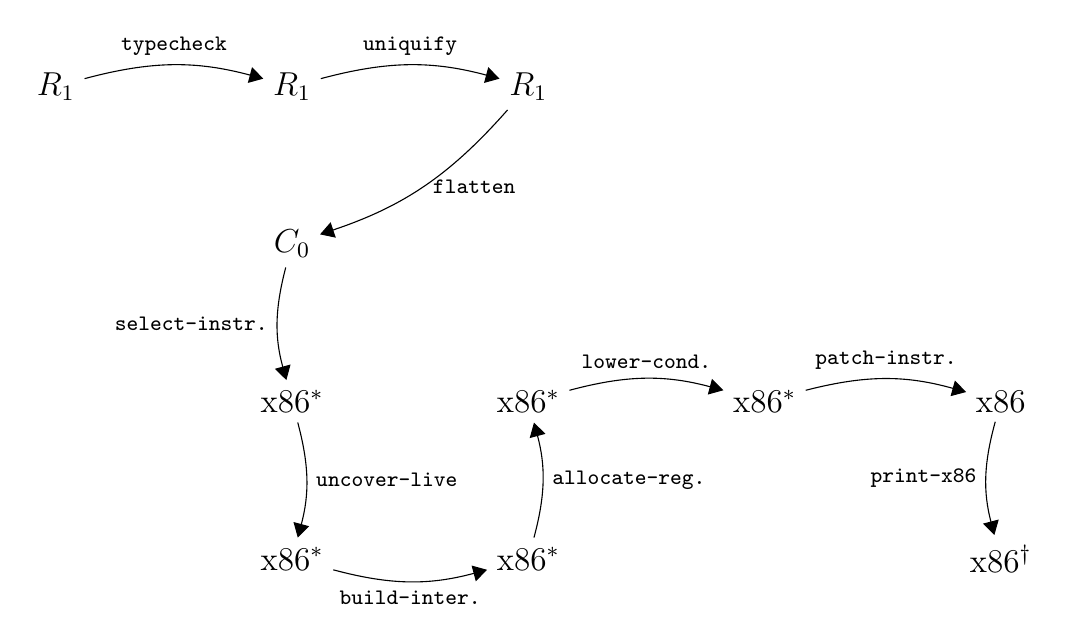
\begin{tikzpicture}[baseline=(current  bounding  box.center)]
\node (R1) at (0,2)  {\large $R_1$};
\node (R1-2) at (3,2)  {\large $R_1$};
\node (R1-3) at (6,2)  {\large $R_1$};
\node (C0-1) at (3,0)  {\large $C_0$};

\node (x86-2) at (3,-2)  {\large $\text{x86}^{*}$};
\node (x86-3) at (6,-2)  {\large $\text{x86}^{*}$};
\node (x86-4) at (9,-2) {\large $\text{x86}^{*}$};
\node (x86-5) at (12,-2) {\large $\text{x86}$};
\node (x86-6) at (12,-4) {\large $\text{x86}^{\dagger}$};

\node (x86-2-1) at (3,-4)  {\large $\text{x86}^{*}$};
\node (x86-2-2) at (6,-4)  {\large $\text{x86}^{*}$};

\path[->,bend left=15] (R1) edge [above] node {\ttfamily\footnotesize typecheck} (R1-2);
\path[->,bend left=15] (R1-2) edge [above] node {\ttfamily\footnotesize uniquify} (R1-3);
\path[->,bend left=15] (R1-3) edge [right] node {\ttfamily\footnotesize flatten} (C0-1);
\path[->,bend right=15] (C0-1) edge [left] node {\ttfamily\footnotesize select-instr.} (x86-2);
\path[->,bend left=15] (x86-2) edge [right] node {\ttfamily\footnotesize uncover-live} (x86-2-1);
\path[->,bend right=15] (x86-2-1) edge [below] node {\ttfamily\footnotesize build-inter.} (x86-2-2);
\path[->,bend right=15] (x86-2-2) edge [right] node {\ttfamily\footnotesize allocate-reg.} (x86-3);
\path[->,bend left=15] (x86-3) edge [above] node {\ttfamily\footnotesize lower-cond.} (x86-4);
\path[->,bend left=15] (x86-4) edge [above] node {\ttfamily\footnotesize patch-instr.} (x86-5);
\path[->,bend right=15] (x86-5) edge [left] node {\ttfamily\footnotesize print-x86} (x86-6);
\end{tikzpicture}
\caption{Diagram of the passes for compiling $R_2$, including the
  new type checking pass.}
\label{fig:R2-passes}
\end{figure}

Figure~\ref{fig:R2-passes} gives an overview of all the passes needed
for the compilation of $R_2$.


\section{Challenge: Optimizing Conditions$^{*}$}
\label{sec:opt-if}

A close inspection of the x86 code generated in
Figure~\ref{fig:if-example-x86} reveals some redundant computation
regarding the condition of the \key{if}. We compare \key{rcx} to $1$
twice using \key{cmpq} as follows.
\begin{lstlisting}
	cmpq	$1, %rcx
	sete	%al
	movzbq	%al, %rcx
	cmpq	$1, %rcx
	je then21288
\end{lstlisting}


The reason for this non-optimal code has to do with the \code{flatten}
pass earlier in this Chapter. We recommended flattening the condition
to an $\Arg$ and then comparing with \code{\#t}. But if the condition
is already an \code{eq?} test, then we would like to use that
directly. In fact, for many of the expressions of Boolean type, we can
generate more optimized code. For example, if the condition is
\code{\#t} or \code{\#f}, we do not need to generate an \code{if} at
all. If the condition is a \code{let}, we can optimize based on the
form of its body. If the condition is a \code{not}, then we can flip
the two branches. 
%
\marginpar{\tiny We could do even better by converting to basic
  blocks.\\ --Jeremy}
%
On the other hand, if the condition is a \code{and}
or another \code{if}, we should flatten them into an $\Arg$ to avoid
code duplication.

Figure~\ref{fig:opt-if} shows an example program and the result of
applying the above suggested optimizations.

\begin{exercise}\normalfont
  Change the \code{flatten} pass to improve the code that gets
  generated for \code{if} expressions. We recommend writing a helper
  function that recursively traverses the condition of the \code{if}.
\end{exercise}

\begin{figure}[tbp]
\begin{tabular}{lll}
\begin{minipage}{0.5\textwidth}
\begin{lstlisting}
(program
  (if (let ([x 1])
        (not (eq? 2 x)))
    42
    777))
\end{lstlisting}
$\Downarrow$
\begin{lstlisting}
(program (x.1 t.1 if.1)
  (assign x.1 1)
  (assign t.1 (read))
  (if (eq? x.1 t.1)
    ((assign if.1 42))
    ((assign if.1 777)))
  (return if.1))
\end{lstlisting}
$\Downarrow$
\begin{lstlisting}
(program (x.1 t.1 if.1)
  (movq (int 1) (var x.1))
  (callq read_int)
  (movq (reg rax) (var t.1))
  (if (eq? (var x.1) (var t.1))
    ((movq (int 42) (var if.1)))
    ((movq (int 777) (var if.1))))
  (movq (var if.1) (reg rax)))
\end{lstlisting}
\end{minipage}
&
$\Rightarrow$
\begin{minipage}{0.4\textwidth}
\begin{lstlisting}
	.globl _main
_main:
	pushq	%rbp
	movq	%rsp, %rbp
	pushq	%r15
	pushq	%r14
	pushq	%r13
	pushq	%r12
	pushq	%rbx
	subq	$8, %rsp
	movq	$1, %rbx
	callq	_read_int
	movq	%rax, %rcx
	cmpq	%rbx, %rcx
	je then21288
	movq	$777, %r12
	jmp if_end21289
then21288:
	movq	$42, %r12
if_end21289:
	movq	%r12, %rax
	movq	%rax, %rdi
	callq	_print_int
	movq	$0, %rax
	addq	$8, %rsp
	popq	%rbx
	popq	%r12
	popq	%r13
	popq	%r14
	popq	%r15
	popq	%rbp
	retq
\end{lstlisting}
\end{minipage}
\end{tabular} 
\caption{Example program with optimized conditionals.}
\label{fig:opt-if}
\end{figure}


%%%%%%%%%%%%%%%%%%%%%%%%%%%%%%%%%%%%%%%%%%%%%%%%%%%%%%%%%%%%%%%%%%%%%%%%%%%%%%%%
\chapter{Tuples and Garbage Collection}
\label{ch:tuples}

In this chapter we study the compilation of mutable tuples (called
``vectors'' in Racket). Figure~\ref{fig:r3-syntax} defines the syntax
for $R_3$, which includes three new forms for creating a tuple,
reading an element of a tuple, and writing an element into a
tuple. The following program shows the usage of tuples in Racket. We
create a 3-tuple \code{t} and a 1-tuple. The 1-tuple is stored at
index $2$ of the 3-tuple, showing that tuples are first-class values.
The element at index $1$ of \code{t} is \code{\#t}, so the ``then''
branch is taken.  The element at index $0$ of \code{t} is $40$, to
which we add the $2$, the element at index $0$ of the 1-tuple.
\begin{lstlisting}
  (let ([t (vector 40 #t (vector 2))])
    (if (vector-ref t 1)
        (+ (vector-ref t 0)
           (vector-ref (vector-ref t 2) 0))
        44))
\end{lstlisting}

Figure~\ref{fig:interp-R3} shows the interpreter for the $R_3$
language. With the addition of the vector operations, there are quite
a few primitive operations and the interpreter code for them is
somewhat repetative. In Figure~\ref{fig:interp-R3} we factor out the
different parts into the \code{interp-op} function and the similar
parts into the one match clause shown in
Figure~\ref{fig:interp-R3}. It is important for that match clause to
come last because it matches \emph{any} compound S-expression.  We do
not use \code{interp-op} for the \code{and} operation because of the
short-circuiting behavior in the order of evaluation of its arguments.

\begin{figure}[tbp]
\begin{lstlisting}
   (define (interp-op op)
     (match op
       ['+ fx+]
       ['- (lambda (n) (fx- 0 n))]
       ['read read-fixnum]
       ['not (lambda (v) (match v [#t #f] [#f #t]))]
       ['eq? (lambda (v1 v2)
               (cond [(or (and (fixnum? v1) (fixnum? v2)) 
                           (and (boolean? v1) (boolean? v2))
                           (and (vector? v1) (vector? v2)))
                      (eq? v1 v2)]))]
       ['vector vector]
       ['vector-ref vector-ref]
       ['vector-set! vector-set!]
       [else (error "in interp-op S0, unmatched" op)]))

   (define (interp-R3 env e)
     (match e
       ...
       [`(,op ,args ...)
        (apply (interp-op op)
                (map (lambda (e) (interp-R3 env e)) args))]
       ))
\end{lstlisting}
\caption{Interpreter for the $R_3$ language. We combine the code for
  most of the primitive operations, including the new vector
  operations, into the one match clause and factor their differences
  into the \code{interp-op} function. }
\label{fig:interp-R3}
\end{figure}

\begin{figure}[tbp]
\centering
\fbox{
\begin{minipage}{0.96\textwidth}
\[
\begin{array}{lcl}
  \Type &::=& \ldots \mid (\key{Vector}\;\Type^{+}) \\
  \Exp &::=& \ldots \mid (\key{vector}\;\Exp^{+}) \mid 
    (\key{vector-ref}\;\Exp\;\Int) \\
  &\mid& (\key{vector-set!}\;\Exp\;\Int\;\Exp)\\
  R_3 &::=& (\key{program} \; \Exp)
\end{array}
\]
\end{minipage}
}
\caption{The $R_3$ language, an extension of $R_2$
  (Figure~\ref{fig:r2-syntax}).}
\label{fig:r3-syntax}
\end{figure}

\begin{figure}[tbp]
\begin{lstlisting}
    (define primitives (set '+ '- 'eq? 'not 'read 
                         'vector 'vector-ref 'vector-set!))

    (define (interp-op op)
      (match op
         ['+ fx+]
         ['- (lambda (n) (fx- 0 n))]
         ['eq? (lambda (v1 v2)
                 (cond [(or (and (fixnum? v1) (fixnum? v2))
                            (and (boolean? v1) (boolean? v2))
                            (and (vector? v1) (vector? v2)))
                        (eq? v1 v2)]))]
         ['not (lambda (v) (match v [#t #f] [#f #t]))]
	 ['read read-fixnum]
         ['vector vector] ['vector-ref vector-ref]
	 ['vector-set! vector-set!]
	 [else (error 'interp-op "unknown operator")]))

   (define (interp-R3 env)
     (lambda (e)
       (match e
         ...
         [`(,op ,args ...) #:when (set-member? primitives op)
           (apply (interp-op op) (map (interp-R3 env) args))]
         [else (error 'interp-R3 "unrecognized expression")]
         )))
\end{lstlisting}
\caption{Interpreter for the $R_3$ language.}
\label{fig:interp-R3}
\end{figure}

Tuples are our first encounter with heap-allocated data, which raises
several interesting issues. First, variable binding performs a
shallow-copy when dealing with tuples, which means that different
variables can refer to the same tuple, i.e., the variables can be
\emph{aliases} for the same thing. Consider the following example in
which both \code{t1} and \code{t2} refer to the same tuple.  Thus, the
mutation through \code{t2} is visible when referencing the tuple from
\code{t1} and the result of the program is therefore \code{42}.
\begin{lstlisting}
(let ([t1 (vector 3 7)])
  (let ([t2 t1])
    (let ([_ (vector-set! t2 0 42)])
      (vector-ref t1 0))))
\end{lstlisting}

The next issue concerns the lifetime of tuples. Of course, they are
created by the \code{vector} form, but when does their lifetime end?
Notice that the grammar in Figure~\ref{fig:r3-syntax} does not include
an operation for deallocating tuples. Furthermore, the lifetime of a
tuple is not tied to any notion of static scoping. For example, the
following program returns \code{3} even though the variable \code{t}
goes out of scope prior to the reference.
\begin{lstlisting}
(vector-ref
  (let ([t (vector 3 7)])
    t)
  0)
\end{lstlisting}
From the perspective of programmer-oberservable behavior, tuples live
forever. Of course, if they really lived forever, then many programs
would run out of memory.\footnote{The $R_3$ language does not have
  looping or recursive function, so it is nie impossible to write a
  program in $R_3$ that will run out of memory. However, we add
  recursive functions in the next Chapter!} A Racket implementation
must therefore perform automatic garbage collection.

\section{Garbage Collection}
\label{sec:GC}

Here we study a relatively simple algorithm for garbage collection
that is the basis of the state-of-the-art generational garbage
collectors~\citep{Lieberman:1983aa,Ungar:1984aa,Jones:1996aa,Detlefs:2004aa,Dybvig:2006aa}. In
particular, we describe a two-space copying
collector~\citep{Wilson:1992fk} that uses Cheney's algorithm to
perform the
copy~\citep{Cheney:1970aa}. Figure~\ref{fig:copying-collector} gives a
coarse-grained depiction of what happens in a two-space collector,
showing two time steps, prior to garbage collection on the top and
after garbage collection on the bottom. In a two-space collector, the
heap is segmented into two parts, the FromSpace and the
ToSpace. Initial, all allocations go to the FromSpace. As you can see,
prior to garbage collection all of the allocated objects are in the
FromSpace.

A running program has direct access to registers and the procedure
call stack, and those may contain pointers into the heap. Those
pointers are called the \emph{root set}. In
Figure~\ref{fig:copying-collector} there are three pointers in the
root set, one in a register and two on the stack. The goal of the
garbage collector is to 1) preserve all objects that are reachable
from the root set via a path of pointers, i.e., the \emph{live}
objects and 2) reclaim the storage of everything else, i.e., the
\emph{garbage}. A copying collector accomplished this by copying all
of the live objects into the ToSpace and then performs a slight of
hand, treating the ToSpace as the new FromSpace and the old FromSpace
as the new ToSpace. In the bottom of
Figure~\ref{fig:copying-collector} you can see the result of the copy.
All of the live objects have been copied to the ToSpace in such a way
that preserves the pointer relationships. For example, the pointer in
the register still points to a 2-tuple whose first element is a
3-tuple and second element is a 2-tuple.

\begin{figure}[tbp]
\centering
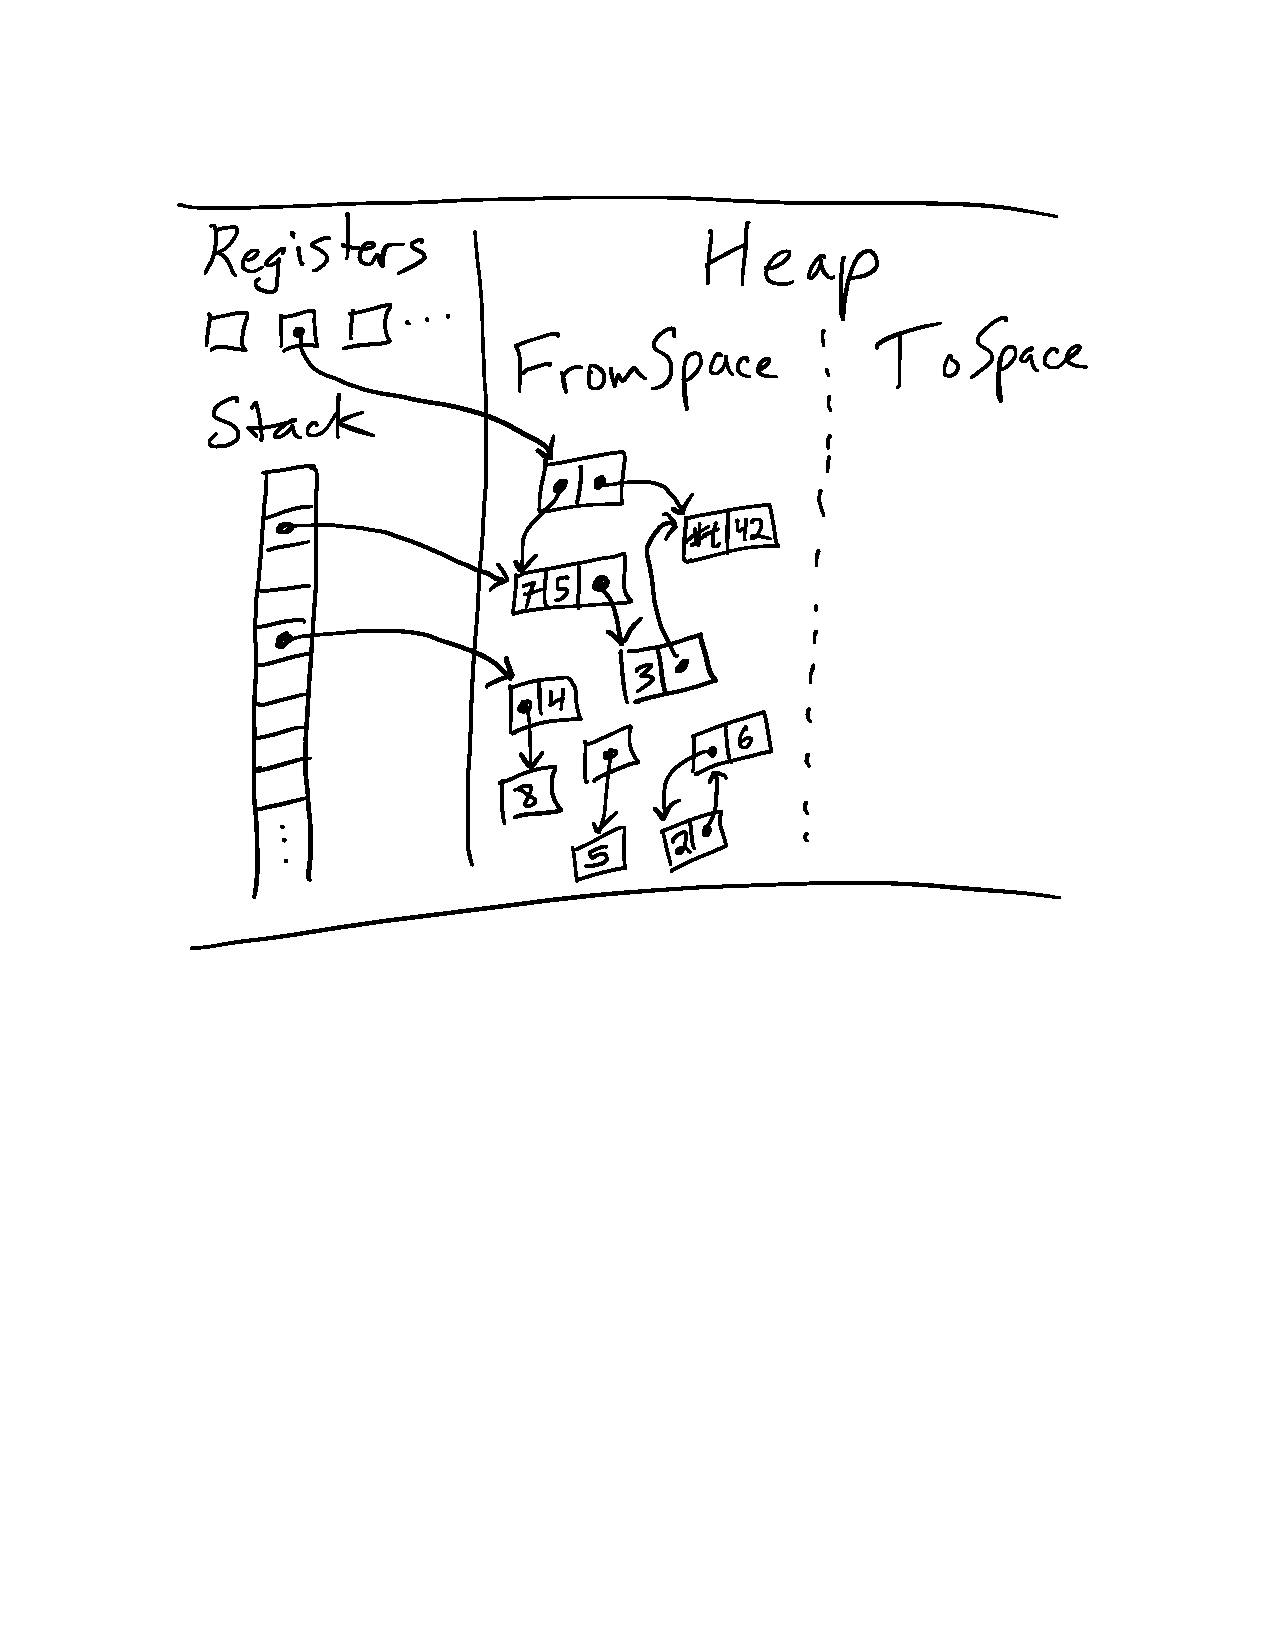
\includegraphics[width=0.9\textwidth]{CopyingCollector} \\
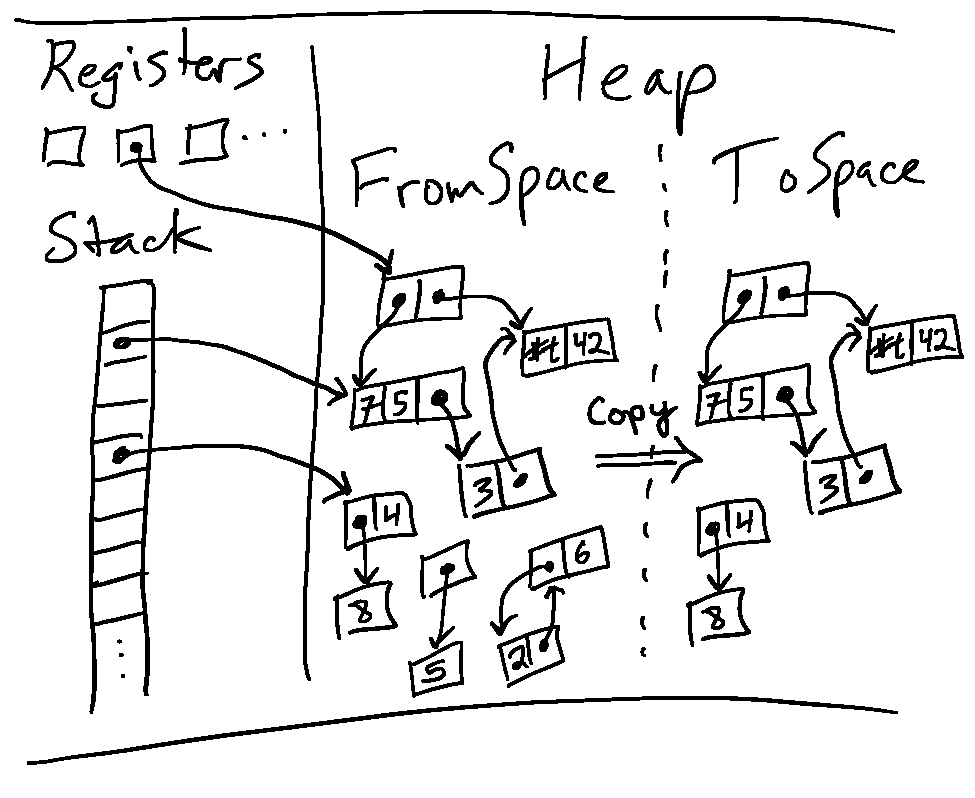
\includegraphics[width=0.9\textwidth]{CopyCollector2}
\caption{A copying collector in action.}
\label{fig:copying-collector}
\end{figure}





\section{Compiler Integration}
\label{sec:compiler-integration}



%%%%%%%%%%%%%%%%%%%%%%%%%%%%%%%%%%%%%%%%%%%%%%%%%%%%%%%%%%%%%%%%%%%%%%%%%%%%%%%%
\chapter{Functions}
\label{ch:functions}

This chapter studies the compilation of functions (aka. procedures) at
the level of abstraction of the C language. The syntax for function
definitions and function application (aka. function call) is shown in
Figure~\ref{fig:r4-syntax}, where we define the $R_4$ language.
Programs in $R_4$ start with zero or more function definitions.  The
function names from these definitions are in-scope for the entire
program, including all other function definitions (so the ordering of
function definitions does not matter).

Functions are first-class in the sense that a function pointer is data
and can be stored in memory or passed as a parameter to another
function.  Thus, we introduce a function type, written
\begin{lstlisting}
   (|$\Type_1$| |$\cdots$| |$\Type_n$| -> |$\Type_r$|)
\end{lstlisting}
for a function whose $n$ parameters have the types $\Type_1$ through
$\Type_n$ and whose return type is $\Type_r$. The main limitation of
these functions (with respect to Racket functions) is that they are
not lexically scoped. That is, the only external entities that can be
referenced from inside a function body are other globally-defined
functions. The syntax of $R_4$ prevents functions from being nested
inside each other; they can only be defined at the top level.

\begin{figure}[tbp]
\centering
\fbox{
\begin{minipage}{0.96\textwidth}
\[
\begin{array}{lcl}
  \Type &::=& \ldots \mid (\Type^{*} \; \key{->}\; \Type) \\
  \Exp &::=& \ldots \mid (\Exp \; \Exp^{*}) \\
  \Def &::=& (\key{define}\; (\Var \; [\Var \key{:} \Type]^{*} \key{:} \Type \; \Exp)) \\
  R_4 &::=& (\key{program} \; \Def^{*} \; \Exp)
\end{array}
\]
\end{minipage}
}
\caption{The $R_4$ language, an extension of $R_3$
  (Figure~\ref{fig:r3-syntax}).}
\label{fig:r4-syntax}
\end{figure}

The program in Figure~\ref{fig:r4-function-example} is a
representative example of defining and using functions in $R_4$.  We
define a function \code{map-vec} that applies some other function
\code{f} to both elements of a vector (a 2-tuple) and returns a new
vector containing the results. We also define a function \code{add1}
that does what its name suggests. The program then applies
\code{map-vec} to \code{add1} and \code{(vector 0 41)}.  The result is
\code{(vector 1 42)}, from which we return the \code{42}.

\begin{figure}[tbp]
\begin{lstlisting}
(program
  (defines
  (define (map-vec [f : (Integer -> Integer)]
                     [v : (Vector Integer Integer)])
          : (Vector Integer Integer)
    (vector (f (vector-ref v 0)) (f (vector-ref v 1))))
  (define (add1 [x : Integer]) : Integer
    (+ x 1))
  (vector-ref (map-vec add1 (vector 0 41)) 1)
  )
\end{lstlisting}
\caption{Example of using functions in $R_4$.}
\label{fig:r4-function-example}
\end{figure}


\marginpar{\scriptsize to do: interpreter for $R_4$. \\ --Jeremy}

\section{Functions in x86}
\label{sec:fun-x86}

The x86 architecture provides a few features to support the
implementation of functions. We have already seen that x86 provides
labels so that one can refer to the location of an instruction, as is
needed for jump instructions. Labels can also be used to mark the
beginning of the instructions for a function.  Going further, we can
obtain the address of a label by using the \key{leaq} instruction and
\key{rip}-relative addressing. For example, the following puts the
address of the \code{add1} label into the \code{rbx} register.
\begin{lstlisting}
   leaq add1(%rip), %rbx
\end{lstlisting}

In Sections~\ref{sec:x86} and \ref{sec:select-s0} we saw the use of
the \code{callq} instruction for jumping to a function as specified by
a label. The use of the instruction changes slightly if the function
is specified by an address in a register, that is, an \emph{indirect
  function call}. The x86 syntax is to give the register name prefixed
with an asterisk.
\begin{lstlisting}
   callq *%rbx
\end{lstlisting}

The x86 architecture does not directly support passing arguments to
functions; instead we use a combination of registers and stack
locations for passing arguments, following the conventions used by
\code{gcc} as described by \cite{Matz:2013aa}. Up to six arguments may
be passed in registers, using the registers \code{rdi}, \code{rsi},
\code{rdx}, \code{rcx}, \code{r8}, and \code{r9}, in that order.  If
there are more than six arguments, then the rest must be placed on the
stack, which we call \emph{stack arguments}, which we discuss in later
paragraphs. The register \code{rax} is for the return value of the
function.

Recall from Section~\ref{sec:x86} that the stack is also used for
local variables, and that at the beginning of a function we move the
stack pointer \code{rsp} down to make room for them.  To make
additional room for passing arguments, we shall move the stack pointer
even further down. We count how many stack arguments are needed for
each function call that occurs inside the body of the function and
find their maximum. Adding this number to the number of local variables
gives us how much the \code{rsp} should be moved at the beginning of
the function. In preparation for a function call, we offset from
\code{rsp} to set up the stack arguments. We put the first stack
argument in \code{0(\%rsp)}, the second in \code{8(\%rsp)}, and so on.

Upon calling the function, the stack arguments are retrieved by the
callee using the base pointer \code{rbp}. The address \code{16(\%rbp)}
is the location of the first stack argument, \code{24(\%rbp)} is the
address of the second, and so on. Figure~\ref{fig:call-frames} shows
the layout of the caller and callee frames. Notice how important it is
that we correctly compute the maximum number of arguments needed for
function calls; if that number is too small then the arguments and
local variables will smash into each other!

As discussed in Section~\ref{sec:print-x86-reg-alloc}, an x86 function
is responsible for following conventions regarding the use of
registers: the caller should assume that all the caller save registers
get overwritten with arbitrary values by the callee. Thus, the caller
should either 1) not put values that are live across a call in caller
save registers, or 2) save and restore values that are live across
calls. We shall recommend option 1).  On the flip side, if the callee
wants to use a callee save register, the callee must arrange to put
the original value back in the register prior to returning to the
caller.


\begin{figure}[tbp]
\centering
\begin{tabular}{r|r|l|l} \hline
Caller View & Callee View & Contents       & Frame \\ \hline
8(\key{\%rbp})  & & return address & \multirow{5}{*}{Caller}\\
0(\key{\%rbp})  &  & old \key{rbp} \\
-8(\key{\%rbp}) &  & variable $1$ \\
\ldots & & \ldots \\
$-8k$(\key{\%rbp}) &  & variable $k$ \\
 & &  \\
$8n-8$\key{(\%rsp)} & $8n+8$(\key{\%rbp})& argument $n$ \\
& \ldots           & \ldots \\
0\key{(\%rsp)} & 16(\key{\%rbp})  & argument $1$   & \\ \hline
& 8(\key{\%rbp})   & return address & \multirow{5}{*}{Callee}\\
& 0(\key{\%rbp})   & old \key{rbp} \\
& -8(\key{\%rbp})  & variable $1$ \\
&  \ldots          & \ldots \\
& $-8m$(\key{\%rsp})   & variable $m$\\ \hline
\end{tabular}

\caption{Memory layout of caller and callee frames.}
\label{fig:call-frames}
\end{figure}


\section{The compilation of functions}

Now that we have a good understanding of functions as they appear in
$R_4$ and the support for functions in x86, we need to plan the
changes to our compiler, that is, do we need any new passes and/or do
we need to change any existing passes? Also, do we need to add new
kinds of AST nodes to any of the intermediate languages?

To begin with, the syntax of $R_4$ is inconvenient for purposes of
compilation because it conflates the use of function names and local
variables and it conflates the application of primitive operations and
the application of functions. This is a problem because we need to
compile the use of a function name differently than the use of a local
variable; we need to use \code{leaq} to move the function name to a
register. Similarly, the application of a function is going to require
a complex sequence of instructions, unlike the primitive
operations. Thus, it is a good idea to create a new pass that changes
function references from just a symbol $f$ to \code{(function-ref
  $f$)} and that changes function application from \code{($e_0$ $e_1$
  $\ldots$ $e_n$)} to the explicitly tagged AST \code{(app $e_0$ $e_1$
  $\ldots$ $e_n$)}. A good name for this pass is
\code{reveal-functions}. Placing this pass after \code{uniquify} is a
good idea, because it will make sure that there are no local variables
and functions that share the same name. On the other hand,
\code{reveal-functions} needs to come before the \code{flatten} pass
because \code{flatten} will help us compiler \code{function-ref}.

Because each \code{function-ref} needs to eventually become an
\code{leaq} instruction, it first needs to become an assignment
statement so there is a left-hand side in which to put the
result. This can be handled easily in the \code{flatten} pass by
categorizing \code{function-ref} as a complex expression.  Then, in
the \code{select-instructions} pass, an assignment of
\code{function-ref} becomes a \code{leaq} instruction as follows: \\
\begin{tabular}{lll}
\begin{minipage}{0.45\textwidth}
\begin{lstlisting}
  (assign |$\itm{lhs}$| (function-ref |$f$|))
\end{lstlisting}
\end{minipage}
&
$\Rightarrow$
&
\begin{minipage}{0.4\textwidth}
\begin{lstlisting}
(leaq (function-ref |$f$|) |$\itm{lhs}$|)
\end{lstlisting}
\end{minipage}
\end{tabular} 

Next we consider compiling function definitions.  The \code{flatten}
pass should handle function definitions a lot like a \code{program}
node; after all, the \code{program} node represents the \code{main}
function. So the \code{flatten} pass, in addition to flattening the
body of the function into a sequence of statements, should record the
local variables in the $\Var^{*}$ field as shown below.
\begin{lstlisting}
   (define (|$f$| [|\itm{xs}| : |\itm{ts}|]|$^{*}$|) : |\itm{rt}| (|$\Var^{*}$|) |$\Stmt^{+}$|)
\end{lstlisting}
In the \code{select-instructions} pass, we need to encode the
parameter passing in terms of the conventions discussed in
Section~\ref{sec:fun-x86}. So depending on the length of the parameter
list \itm{xs}, some of them may be in registers and some of them may
be on the stack. I recommend generating \code{movq} instructions to
move the parameters from their registers and stack locations into the
variables \itm{xs}, then let register allocation handle the assignment
of those variables to homes. After this pass, the \itm{xs} can be
added to the list of local variables. As mentioned in
Section~\ref{sec:fun-x86}, we need to find out how far to move the
stack pointer to ensure we have enough space for stack arguments in
all the calls inside the body of this function. This pass is a good
place to do this and store the result in the \itm{maxStack} field of
the output \code{define} shown below.
\begin{lstlisting}
  (define (|$f$|) |\itm{numParams}| (|$\Var^{*}$| |\itm{maxStack}|) |$\Instr^{+}$|)
\end{lstlisting}

Next, consider the compilation of function applications, which have
the following form at the start of \code{select-instructions}.
\begin{lstlisting}
  (assign |\itm{lhs}| (app |\itm{fun}| |\itm{args}| |$\ldots$|))
\end{lstlisting}
In the mirror image of handling the parameters of function
definitions, some of the arguments \itm{args} need to be moved to the
argument passing registers and the rest should be moved to the
appropriate stack locations, as discussed in
Section~\ref{sec:fun-x86}. You might want to introduce a new kind of
AST node for stack arguments, \code{(stack-arg $i$)} where $i$ is the
index of this argument with respect to the other stack arguments. As
you're generate this code for parameter passing, take note of how many
stack arguments are needed for purposes of computing the
\itm{maxStack} discussed above.

Once the instructions for parameter passing have been generated, the
function call itself can be performed with an indirect function call,
for which I recommend creating the new instruction
\code{indirect-callq}. Of course, the return value from the function
is stored in \code{rax}, so it needs to be moved into the \itm{lhs}.
\begin{lstlisting}
  (indirect-callq |\itm{fun}|)
  (movq (reg rax) |\itm{lhs}|)
\end{lstlisting}

The rest of the passes need only minor modifications to handle the new
kinds of AST nodes: \code{function-ref}, \code{indirect-callq}, and
\code{leaq}. Inside \code{uncover-live}, when computing the $W$ set
(written variables) for an \code{indirect-callq} instruction, I
recommend including all the caller save registers, which will have the
affect of making sure that no caller save register actually need to be
saved. In \code{patch-instructions}, you should deal with the x86
idiosyncrasy that the destination argument of \code{leaq} must be a
register.

For the \code{print-x86} pass, I recommend the following translations:
\begin{lstlisting}
  (function-ref |\itm{label}|) |$\Rightarrow$| |\itm{label}|(%rip)
  (indirect-callq |\itm{arg}|) |$\Rightarrow$| callq *|\itm{arg}|
  (stack-arg |$i$|) |$\Rightarrow$| |$i$|(%rsp)
\end{lstlisting}
For function definitions, the \code{print-x86} pass should add the
code for saving and restoring the callee save registers, if you
haven't already done that.

\section{An Example Translation}

Figure~\ref{fig:add-fun} shows an example translation of a simple
function in $R_4$ to x86. The figure includes the results of the
\code{flatten} and \code{select-instructions} passes.  Can you see any
obvious ways to improve the translation?

\begin{figure}[tbp]
\begin{tabular}{lll}
\begin{minipage}{0.5\textwidth}
\begin{lstlisting}
(program
 (define (add [x : Integer] 
                [y : Integer]) 
    : Integer (+ x y))
 (add 40 2))
\end{lstlisting}
$\Downarrow$
\begin{lstlisting}
(program (t.1 t.2)
  (defines 
    (define (add.1 [x.1 : Integer] 
                    [y.1 : Integer])
      : Integer (t.3)
      (assign t.3 (+ x.1 y.1))
      (return t.3)))
  (assign t.1 (function-ref add.1))
  (assign t.2 (app t.1 40 2))
  (return t.2))
\end{lstlisting}
$\Downarrow$
\begin{lstlisting}
(program ((t.1 t.2) 0)
  ((define (add.1) 2 ((x.1 y.1 t.3) 0)
     (movq (reg rdi) (var x.1))
     (movq (reg rsi) (var y.1))
     (movq (var x.1) (var t.3))
     (addq (var y.1) (var t.3))
     (movq (var t.3) (reg rax))))
  (leaq (function-ref add.1) (var t.1))
  (movq (int 40) (reg rdi))
  (movq (int 2) (reg rsi))
  (indirect-callq (var t.1))
  (movq (reg rax) (var t.2))
  (movq (var t.2) (reg rax)))
\end{lstlisting}
\end{minipage}
&
\begin{minipage}{0.4\textwidth}
$\Downarrow$
\begin{lstlisting}
	.globl add_1
add_1:
	pushq	%rbp
	movq	%rsp, %rbp
	pushq	%r15
	pushq	%r14
	pushq	%r13
	pushq	%r12
	pushq	%rbx
	subq	$16, %rsp
	movq	%rdi, %rbx
	movq	%rsi, %rcx
	addq	%rcx, %rbx
	movq	%rbx, %rax
	addq	$16, %rsp
	popq	%rbx
	popq	%r12
	popq	%r13
	popq	%r14
	popq	%r15
	popq	%rbp
	retq

	.globl _main
_main:
	pushq	%rbp
	movq	%rsp, %rbp
	subq	$16, %rsp
	leaq	add_1(%rip), %rbx
	movq	$40, %rdi
	movq	$2, %rsi
	callq	*%rbx
	movq	%rax, %rbx
	movq	%rbx, %rax
	addq	$16, %rsp
	popq	%rbp
	retq
\end{lstlisting}
\end{minipage}
\end{tabular} 
\caption{Example compilation of a simple function to x86.}
\label{fig:add-fun}
\end{figure}



\begin{exercise}\normalfont
Expand your compiler to handle $R_4$ as outlined in this section.
Create 5 new programs that use functions, including examples that pass
functions and return functions from other functions, and test your
compiler on these new programs and all of your previously created test
programs.
\end{exercise}


%%%%%%%%%%%%%%%%%%%%%%%%%%%%%%%%%%%%%%%%%%%%%%%%%%%%%%%%%%%%%%%%%%%%%%%%%%%%%%%%
\chapter{Lexically Scoped Functions}
\label{ch:lambdas}

\begin{figure}[tbp]
\centering
\fbox{
\begin{minipage}{0.96\textwidth}
\[
\begin{array}{lcl}
  \Exp &::=& \ldots \mid (\key{lambda:}\; ([\Var \key{:} \Type]^{*} \key{:} \Type \; \Exp)) \\
  R_5 &::=& (\key{program} \; \Def^{*} \; \Exp)
\end{array}
\]
\end{minipage}
}
\caption{The $R_5$ language, an extension of $R_4$
  (Figure~\ref{fig:r4-syntax}).}
\label{fig:r5-syntax}
\end{figure}


%%%%%%%%%%%%%%%%%%%%%%%%%%%%%%%%%%%%%%%%%%%%%%%%%%%%%%%%%%%%%%%%%%%%%%%%%%%%%%%%
%\chapter{Mutable Data}
%\label{ch:mutable-data}

%%%%%%%%%%%%%%%%%%%%%%%%%%%%%%%%%%%%%%%%%%%%%%%%%%%%%%%%%%%%%%%%%%%%%%%%%%%%%%%%
\chapter{Dynamic Typing}
\label{ch:type-dynamic}


%%%%%%%%%%%%%%%%%%%%%%%%%%%%%%%%%%%%%%%%%%%%%%%%%%%%%%%%%%%%%%%%%%%%%%%%%%%%%%%%
\chapter{Parametric Polymorphism}
\label{ch:parametric-polymorphism}

%%%%%%%%%%%%%%%%%%%%%%%%%%%%%%%%%%%%%%%%%%%%%%%%%%%%%%%%%%%%%%%%%%%%%%%%%%%%%%%%
\chapter{High-level Optimization}
\label{ch:high-level-optimization}

%%%%%%%%%%%%%%%%%%%%%%%%%%%%%%%%%%%%%%%%%%%%%%%%%%%%%%%%%%%%%%%%%%%%%%%%%%%%%%%%
\chapter{Appendix}

\section{Interpreters}
\label{appendix:interp}

We provide several interpreters in the \key{interp.rkt} file.  The
\key{interp-scheme} function takes an AST in one of the Racket-like
languages considered in this book ($R_1, R_2, \ldots$) and interprets
the program, returning the result value.  The \key{interp-C} function
interprets an AST for a program in one of the C-like languages ($C_0,
C_1, \ldots$), and the \code{interp-x86} function interprets an AST
for an x86 program.

\section{Utility Functions}
\label{appendix:utilities}

The utility function described in this section can be found in the
\key{utilities.rkt} file.

The \key{read-program} function takes a file path and parses that file
(it must be a Racket program) into an abstract syntax tree (as an
S-expression) with a \key{program} AST at the top.

The \key{assert} function displays the error message \key{msg} if the
Boolean \key{bool} is false.
\begin{lstlisting}
(define (assert msg bool) ...)
\end{lstlisting}

The \key{lookup} function ...

The \key{map2} function ...


\subsection{Graphs}

\begin{itemize}
\item The \code{make-graph} function takes a list of vertices
  (symbols) and returns a graph.

\item The \code{add-edge} function takes a graph and two vertices and
  adds an edge to the graph that connects the two vertices. The graph
  is updated in-place. There is no return value for this function.

\item The \code{adjacent} function takes a graph and a vertex and
  returns the set of vertices that are adjacent to the given
  vertex. The return value is a Racket \code{hash-set} so it can be
  used with functions from the \code{racket/set} module.

\item The \code{vertices} function takes a graph and returns the list
  of vertices in the graph.
\end{itemize}

\subsection{Testing}

The \key{interp-tests} function takes a compiler name (a string), a
description of the passes, an interpreter for the source language, a
test family name (a string), and a list of test numbers, and runs the
compiler passes and the interpreters to check whether the passes
correct. The description of the passes is a list with one entry per
pass.  An entry is a list with three things: a string giving the name
of the pass, the function that implements the pass (a translator from
AST to AST), and a function that implements the interpreter (a
function from AST to result value) for the language of the output of
the pass.  The interpreters from Appendix~\ref{appendix:interp} make a
good choice.  The \key{interp-tests} function assumes that the
subdirectory \key{tests} has a bunch of Scheme programs whose names
all start with the family name, followed by an underscore and then the
test number, ending in \key{.scm}. Also, for each Scheme program there
is a file with the same number except that it ends with \key{.in} that
provides the input for the Scheme program.
\begin{lstlisting}
(define (interp-tests name passes test-family test-nums) ...
\end{lstlisting}

The compiler-tests function takes a compiler name (a string) a
description of the passes (see the comment for \key{interp-tests}) a
test family name (a string), and a list of test numbers (see the
comment for interp-tests), and runs the compiler to generate x86 (a
\key{.s} file) and then runs gcc to generate machine code.  It runs
the machine code and checks that the output is 42.
\begin{lstlisting}
(define (compiler-tests name passes test-family test-nums) ...)
\end{lstlisting}

The compile-file function takes a description of the compiler passes
(see the comment for \key{interp-tests}) and returns a function that,
given a program file name (a string ending in \key{.scm}), applies all
of the passes and writes the output to a file whose name is the same
as the program file name but with \key{.scm} replaced with \key{.s}.
\begin{lstlisting}
(define (compile-file passes)
  (lambda (prog-file-name) ...))
\end{lstlisting}

\bibliographystyle{plainnat}
\bibliography{all}

\end{document}

%%  LocalWords:  Dybvig Waddell Abdulaziz Ghuloum Dipanwita Sussman
%%  LocalWords:  Sarkar lcl Matz aa representable Chez Ph Dan's nano
%%  LocalWords:  fk bh Siek plt uq Felleisen Bor Yuh ASTs AST Naur eq
%%  LocalWords:  BNF fixnum datatype arith prog backquote quasiquote
%%  LocalWords:  ast sexp Reynold's reynolds interp cond fx evaluator
%%  LocalWords:  quasiquotes pe nullary unary rcl env lookup gcc rax
%%  LocalWords:  addq movq callq rsp rbp rbx rcx rdx rsi rdi subq nx
%%  LocalWords:  negq pushq popq retq globl Kernighan uniquify lll ve
%%  LocalWords:  allocator gensym alist subdirectory scm rkt tmp lhs
%%  LocalWords:  runtime Liveness liveness undirected Balakrishnan je
%%  LocalWords:  Rosen DSATUR SDO Gebremedhin Omari morekeywords cnd
%%  LocalWords:  fullflexible vertices Booleans Listof Pairof thn els
%%  LocalWords:  boolean typecheck notq cmpq sete movzbq jmp al
%%  LocalWords:  EFLAGS thns elss elselabel endlabel Tuples tuples os
%%  LocalWords:  tuple args lexically leaq Polymorphism msg bool nums
%%  LocalWords:  macosx unix Cormen vec callee xs maxStack numParams
%%  LocalWords:  arg
